

\setlength{\overviewextra}{2pt}
\addtolength{\columnsep}{\overviewextra}
\begin{overview}[-25pt]
\phantomsection\label{overview:SUPER}
Tax breaks for superannuation contributions and earnings should be targeted more tightly at their policy purpose. The current system is expensive and unfair. 

Superannuation tax breaks mean that less tax is paid on super savings than is paid on other forms of income. These tax breaks should only be available when they serve a policy aim. Although the \$2~trillion superannuation system does not have legislated aims, most believe it should encourage savings to supplement or replace the Age Pension. 

Yet superannuation tax breaks often go well beyond this purpose and their costs are unsustainable. The tax breaks reduce income tax collections by more than \$25~billion a year. More than half the benefits flow to the wealthiest 20~per~cent of households who already have enough resources to fund their own retirement, and whose savings choices aren’t affected much by tax rates. 

Three reforms are needed to target superannuation better.

\textbf{‘Concessional contributions’} made from pre-tax income should be limited to \$11,000 per year. Eighty per cent of contributions above this level come from the 20~per~cent of taxpayers with the highest incomes, people likely to retire with enough assets to be ineligible for an Age Pension. This change would improve budget balances by \$3.5~billion a year. Other options, such as levying higher taxes on contributions made by higher income earners, would be less well targeted and more complex to administer. Replacing the annual cap with a lifetime cap sounds attractive because it appears to allow people with broken work histories to catch up, but it would mainly turbocharge tax planning for wealthy older workers.

\textbf{‘Non-concessional contributions’} made from post-tax income
should  be limited to \$250,000 over a lifetime. Of the \$33~billion in
post-tax contributions each year, around half are made by just
200,000 people who already have at least \$500,000 in super.


\textbf{Earnings in retirement} – currently untaxed – should be taxed at 15~per~cent, the same as superannuation earnings before retirement. More than half of the benefit of tax-free earnings in retirement goes to the wealthiest 20~per~cent of retirees. For the top 10~per~cent of over 60s drawing on super, the tax benefits are extremely generous – they pay no tax on their average super earnings of \$85,000 a year. A 15~per~cent tax on all super earnings would improve budget balances by {\$2.7~billion} a year today, and much more in future. 

The proposed reforms are fair. Low-income earners and younger people would pay less in other taxes if super tax breaks for the wealthy were wound back. Those already retired would pay some tax on their superannuation savings, but they would pay much less tax than wage earners on similar incomes. For a small proportion of women with higher incomes later in life, the changes would reduce their catch-up contributions. Yet the changes would reduce the tax breaks far more for a lot of rich old men. 

The changes to contributions taxes would be prospective. The changes to earnings tax rates, like changes to income tax rates, would apply to future earnings of assets already acquired.

\end{overview}
\addtolength{\columnsep}{-\overviewextra}
% \contentspage

\chapter{Introduction}
\section{We have a budget problem}
Grattan Institute’s 2013 report, \citetitle{DaleyMcGannonSavage2013BudgetPressures}, concluded that without structural reforms Australian governments could face a decade of deficits.  \Cref{part:FISCAL} showed that this may have been optimistic. 

The Commonwealth Government has run deficits for six years, largely due to a rapid increase in net spending on older households. The costs of repaying these deficits will fall primarily on younger households.%\oneraggedpage

The next ten years are likely to be even more difficult. Falling terms of trade and lower nominal economic growth will drag on revenues at the same time the Commonwealth Government intends to fund substantial new policy initiatives.

The Commonwealth Government is yet to respond to the scale of its budget challenges. In office, both major political parties have hoped that bracket creep and favourable economic conditions would deliver a surplus. Hope is the key word: over the last six years, outcomes have consistently been worse than these projections. The latest short- and medium-term projections rely on optimistic assumptions about organic revenue growth and spending restraint. If any of them fail to materialise, the burden on younger generations will increase.

\section{Previous Grattan work has identified pensions and superannuation policy as priorities for budget repair}\label{sec:SUPER-prev-grattan-work-identified-super}
Balancing budgets identified better targeting of pension and superannuation policies as being among the best opportunities to achieve budget~repair.\footcite[][29]{DaleyMcGannonSavage2013BudgetPressures}

The key choices identified were increasing the age of access for the Age Pension and superannuation, limiting tax concessions for superannuation, and including owner-occupied housing in the Age Pension assets test. Although a government is unlikely to make all these choices simultaneously, we estimated in \citetitle{DaleyMcGannonSavageEtAl2013BalancingBudgets} that they could collectively improve the budget bottom line by an estimated \$27~billion a year. 

Obviously these choices primarily affect older Australians in the short term. They emerged as high priorities because tax and welfare policies for older Australians are less well-targeted to those most in need than are other policies. Consequently it is easier to identify changes that deliver substantial improvements to the budget with relatively few side-effects. These choices will affect all Australians as they age, not just the current older generation. 

\section{\mbox{Older households are putting the most pressure on Australian budgets}}
Budget measures that affect older Australians may also be appropriate because older Australians are putting most pressure on government budgets. Grattan’s 2014 report, \citetitle{DaleyMcGannonHunter2014}, showed how the largest spending increases over the last decade have been increased spending in health (where governments spend twice as much on each 60 year old as a 30 year old\footcite[][25]{DaleyMcGannonHunter2014}) and on the Age Pension. Both of these spending categories grew substantially faster than GDP, not because of the ageing population, but because of explicit and implicit choices to spend more per person of a given age.

\begin{figure}[htp]
\captionwithunits{The generational bargain transfers substantial resources from younger to older households}%
{Average net benefits per household, 1988-89 to 2009-10 (2010 dollars)}\label{fig:SUPER-Wealth-of-generations-chart}
\includegraphics[width=\columnwidth]{super-atlas/Figure1-from-atlas-1.pdf}
\notes{Based on the HES surveys of 1988-89, 1993-94, 1998-99. 2003-04 and 2009-10. Net benefits are social assistance benefits in cash, plus support in kind, minus income and sales taxes. Age is by age of household reference person.}

\source{Figure~3.1 in \citetitle{DaleyWoodWeidmannEtAl2014}.}
\end{figure}

Grattan Institute’s report, \citetitle{DaleyWoodWeidmannEtAl2014}, argued that Australia’s intergenerational fiscal bargain was coming under threat as younger generations were being asked to do more than their fair share. \Vref{fig:SUPER-Wealth-of-generations-chart} shows how Commonwealth and state governments combined spent \$9,400 more per household aged over 65 in 2010 than they did six years earlier, reflecting increases in the Age Pension and rising health spending per person.\footcite[][22]{DaleyWoodWeidmannEtAl2014}  At the same time, average income taxes paid by those aged 65 and over fell in real dollar terms, despite higher incomes, reflecting the decision by the former Howard Government to abolish taxes on superannuation withdrawals for over 60s and to increase the effective tax-free threshold to \$30,000 for retirees’ earnings outside of superannuation. These budgetary decisions have been funded by deficits. The accumulating debt burden will disproportionately fall on younger households.\footcite[][29]{DaleyWoodWeidmannEtAl2014}


Transitioning to a fairer set of policies requires careful thought. Younger generations, on the wrong side of the drawbridge after the policies change, lose out when they pay for benefits for older generations that they do not receive themselves. If government reduces spending on health, pensions and superannuation tax breaks, then younger generations will be disadvantaged. Exempting older households from the costs of policy changes – such as by grandfathering existing benefits and tax breaks – simply magnifies the costs shifted onto younger generations. 

\section{Re-targeting superannuation tax breaks would help fix the budget, and restore the intergenerational bargain}
This report shows how tax breaks for superannuation contributions and earnings should be targeted more tightly at their policy purpose. The current system is expensive and unfair. They are the largest and fastest growing leaks from our income tax system, reducing income tax collections by over \$25~billion a year. 

Better targeting of tax breaks on superannuation contributions could save \$3.5~billion a year. Restoring taxes on superannuation fund earnings for those in retirement – as already applies for workers – could raise another \$2.7~billion a year today, and much more as more people retire. 

Better targeting superannuation tax breaks would also reduce the transfers between today’s younger taxpayers and older retirees. Taxes on super earnings in retirement, for example, would most affect those who have benefited from windfalls, government largesse and paying lower taxes while deficits accumulated.

Over the last decade, older households captured most of the growth in Australia’s wealth. Despite the global financial crisis, households aged between 65 and 74 years today are \$400,000 (or 27~per~cent) wealthier in real terms than households of that age were ten years ago. Meanwhile, the wealth of households aged 25 to 34 years fell by \$2,000 (or 4~per~cent).\footnote{\gao\ \textcites{ABS2015HouseholdIncomeWealth1314}{ABS2006HES0304}.}

\section{What this report does not do}\label{sec:SUPER-what-this-report-does-not-do}
This report focuses on what changes are needed to better align the tax treatment of superannuation with the overall objectives of our superannuation system, and to support budget repair. 

This report does not advocate \textbf{wholesale restructuring of the tax treatment of retirement savings. }

Private retirement savings can be taxed at three points: on contributions; investment earnings; and withdrawals. Each stage in the life of an asset can be described as being either: fully taxed at marginal rates of personal income tax (\taxabbrevT); taxed more lightly than marginal rates (\taxabbrevt); or exempt from tax (\taxabbrevE). Australia currently has a \ttE\ approach to taxing most super savings.\index{TEE,EET,ttE}

A number of commentators have highlighted the benefits of moving to an expenditure tax treatment of retirement savings.  The two most common expenditure tax approaches, detailed in \Cref{appendix:SUPER-approaches-measures-for-tax-rates-on-savings}, are: 
\begin{enumerate}
\item \textbf{a post-paid expenditure tax (\EET)} where contributions and earnings are tax-exempt, but withdrawals are taxed at a person's marginal tax rate; and
\item \textbf{a pre-paid expenditure tax (\TEE)} where contributions are taxed at marginal rates of personal income tax, but earnings and benefits are tax-exempt. 
\end{enumerate}

While there are theoretical reasons to prefer an \EET\ system over a \TEE\ system – for example an \EET\ system makes it is simpler to tax retirement savings progressively – the costs of transitioning from a system such as Australia’s are prohibitive.\footnote{Australia had an \EET\ system for pre-tax superannuation contributions until 1988 when the Hawke Government introduced taxes on super contributions and earnings, and reduced taxes on super withdrawals, creating a `\ttt' system. The Howard Government abolished taxes on super withdrawals in 2007, creating our present \ttE\ system, \textcite[][44]{Treasury2008RetirementIncomeConsultPaper}.} Either there would be large windfall losses for the generation affected by the transition, or government would need to put in place and maintain complex transitional arrangements (which impose dead-weight administrative costs) for decades. Shifting to an \EET\ system would also lead to substantial short-term revenue shortfalls for Commonwealth governments.\footnote{\textcite{Mercer2015SubmissionToReThink}. For example, the Commonwealth Government expects to collect \$6.1 billion in superannuation taxes in 2014-15. \textcite[][5]{Treasury2015FinalBudgetOutcome1415}.}

The alternative, moving to a \TEE\ system,\footnote{As proposed by \textcites{MaddockKing2015}{Freebairn2015a}.} would impose the greatest costs on younger generations that would pay much higher taxes on their super contributions. A \TEE\ system would also provide a windfall to older generations that contributed most of their superannuation savings at concessional rates under the current \ttE\ system. It would further undermine the intergenerational fiscal bargain already threatened by sharply reduced taxes and higher public spending for older Australians that has occurred over the past decade.\footcite[][2]{DaleyWoodWeidmannEtAl2014} 

A common feature of expenditure tax approaches is that, unlike Australia’s superannuation system, they do not tax the earnings on savings. Taxing the earnings on savings reduces the incentives to save. This might be justified if it discourages economic activity less than alternative taxes. Taxes on savings may also be a means to a greater degree of redistribution of income and wealth. Obviously the degree of progressivity in the tax system is a value choice that is contested.\footcite{Davidson2015} 

This report does not deal with \textbf{harmonising the tax treatment of different savings vehicles} in Australia. The different tax treatments lead to distortions in the allocation of savings.  Aligning the tax treatment of savings income across different savings vehicles, as highlighted in the Henry Tax Review, is an important avenue for future reform. However, current budget pressures make it unlikely that the Commonwealth Government will be prepared to collect less from more highly taxed savings vehicles in the near term.

Although investigating the variety of tax treatments for savings is beyond the scope of this report, on any view, superannuation is an outlier, treated much more generously and much less progressively than other savings vehicles (\Vref{fig:SUPER-2-3}).

This report also does not advocate reforms to \textbf{other components of Australia’s retirement income system}. Responding to the challenges and opportunities of an ageing population and longer life expectancy requires a holistic review of Australia’s retirement incomes system. A comprehensive review of retirement incomes policy is beyond the scope of this report. As already noted \DEVIATION{in \Cref{sec:SUPER-prev-grattan-work-identified-super}}, previous Grattan reports have identified other potential reforms to better target pensions and superannuation policy, such as better targeting access to the Age Pension, and aligning the preservation ages for super and the Age Pension. Future Grattan Institute reports will explore these reforms in greater detail. 

\section{\mbox{The report shows how superannuation currently works, and how it should work}}
The following chapters describe in more detail how superannuation works and what its objectives should be. Later chapters consider how existing superannuation tax breaks do (and don’t) serve the purposes of superannuation and assess options for reform.

Chapter 2 examines the \textbf{role and cost of superannuation tax breaks}. It considers how the overall objectives of the superannuation system have evolved and what the objectives should now be.

Chapter 3 examines the \textbf{distribution of superannuation tax breaks overall} and assesses how much superannuation people need to sustain a comfortable retirement.  

Chapter 4 examines the tax breaks for \textbf{pre-tax contributions} to superannuation. These allow people to save into superannuation from their pre-tax income.

Chapter 5 examines \textbf{how much in total people can contribute} to superannuation, including from their post-tax income. The more that a person saves through superannuation, the less tax they pay on the earnings on savings.

Chapter 6 examines \textbf{how much tax is paid on superannuation earnings}. It focuses on provisions that result in no tax on super fund earnings in retirement.

%
%
%
\chapter{The role and cost of superannuation tax breaks}
Superannuation provides a number of tax breaks. Relative to saving outside of superannuation, less tax is paid on money saved into superannuation, and less tax is paid on the earnings.

The purposes of these tax breaks are contested because the broader purposes of superannuation are poorly defined. The best analysis is that the tax breaks aim to encourage savings that will supplement or replace the Age Pension. 

Superannuation tax breaks provide additional incentives to save. They also recognise that superannuation compels people to save, and locks up voluntary contributions until retirement.

Some analyses suggest that superannuation tax breaks are needed because high-income earners paying income tax on the earnings of their savings would not have enough incentives to save. However, even taxpayers on the top marginal rate of income tax have reasonable incentives to save for more consumption tomorrow rather than to consume more  today.

In any case, many people, particularly high-income earners, save in order to smooth lifetime incomes or to provide a legacy. Evidence from around the world, confirmed by our analysis of the Australian system, suggests that these taxpayers will tend to save about the same amount, irrespective of the taxes on earnings.

\oneraggedpage

Whatever the benefits of superannuation tax breaks, they must be balanced against the costs – not least the budgetary costs, and the costs of other taxes being higher. Superannuation tax breaks cost a lot – over 10 per cent of income tax collections – and the cost is growing fast.

\section{Superannuation savings are the least important pillar of Australia's retirement income system}\label{sec:SUPER-Super-savings-are-least-important-pillar}\label{sec:SUPER-2-1}
Superannuation savings form part of Australia four-pillar retirement income system, which is made up of:%
\footnote{%
Some authors identify three pillars in the retirement income system, either by combining all superannuation savings into one pillar, or separating out compulsory and voluntary superannuation savings but ignoring voluntary savings beyond superannuation such as housing assets (see \textcite[][9]{Treasury2009aftsRetirementIncomeStrategicIssues}). More recent approaches distinguish between compulsory and voluntary superannuation savings, and note the importance of voluntary savings outside the superannuation system (\textcite[][17]{Derby2015}). 
}%
\mynobreakpar
\begin{enumerate}
\item The \textbf{means-tested Age Pension}, provided by government, which guarantees a minimum `safety net' level of income in retirement.
\item \textbf{Compulsory saving through the \emph{Superannuation Guarantee}}, currently set at 9.5~per cent of wages.
\item \textbf{Voluntary superannuation savings}, including voluntary pre-tax and post-tax super contributions.
\item \textbf{Other voluntary savings} that can contribute towards living standards in retirement, such as other financial assets, and especially housing and other property.
\end{enumerate}

Australia’s four-pillar retirement system is well regarded internationally. It spreads the responsibility and risk of providing retirement incomes in a fiscally sustainable way, and has helped Australia deal with the challenges of an ageing population.\footcite{Mercer2015} 

\begin{figure}
\captionwithunits{Superannuation is the least important `pillar' in Australia's retirement incomes system}%
{Mean wealth per household by type and age, (2013-14 dollars)}\label{fig:SUPER-2-1}
% 
\includegraphics[width=\columnwidth, page=5]{super-atlas/PPTX.pdf}
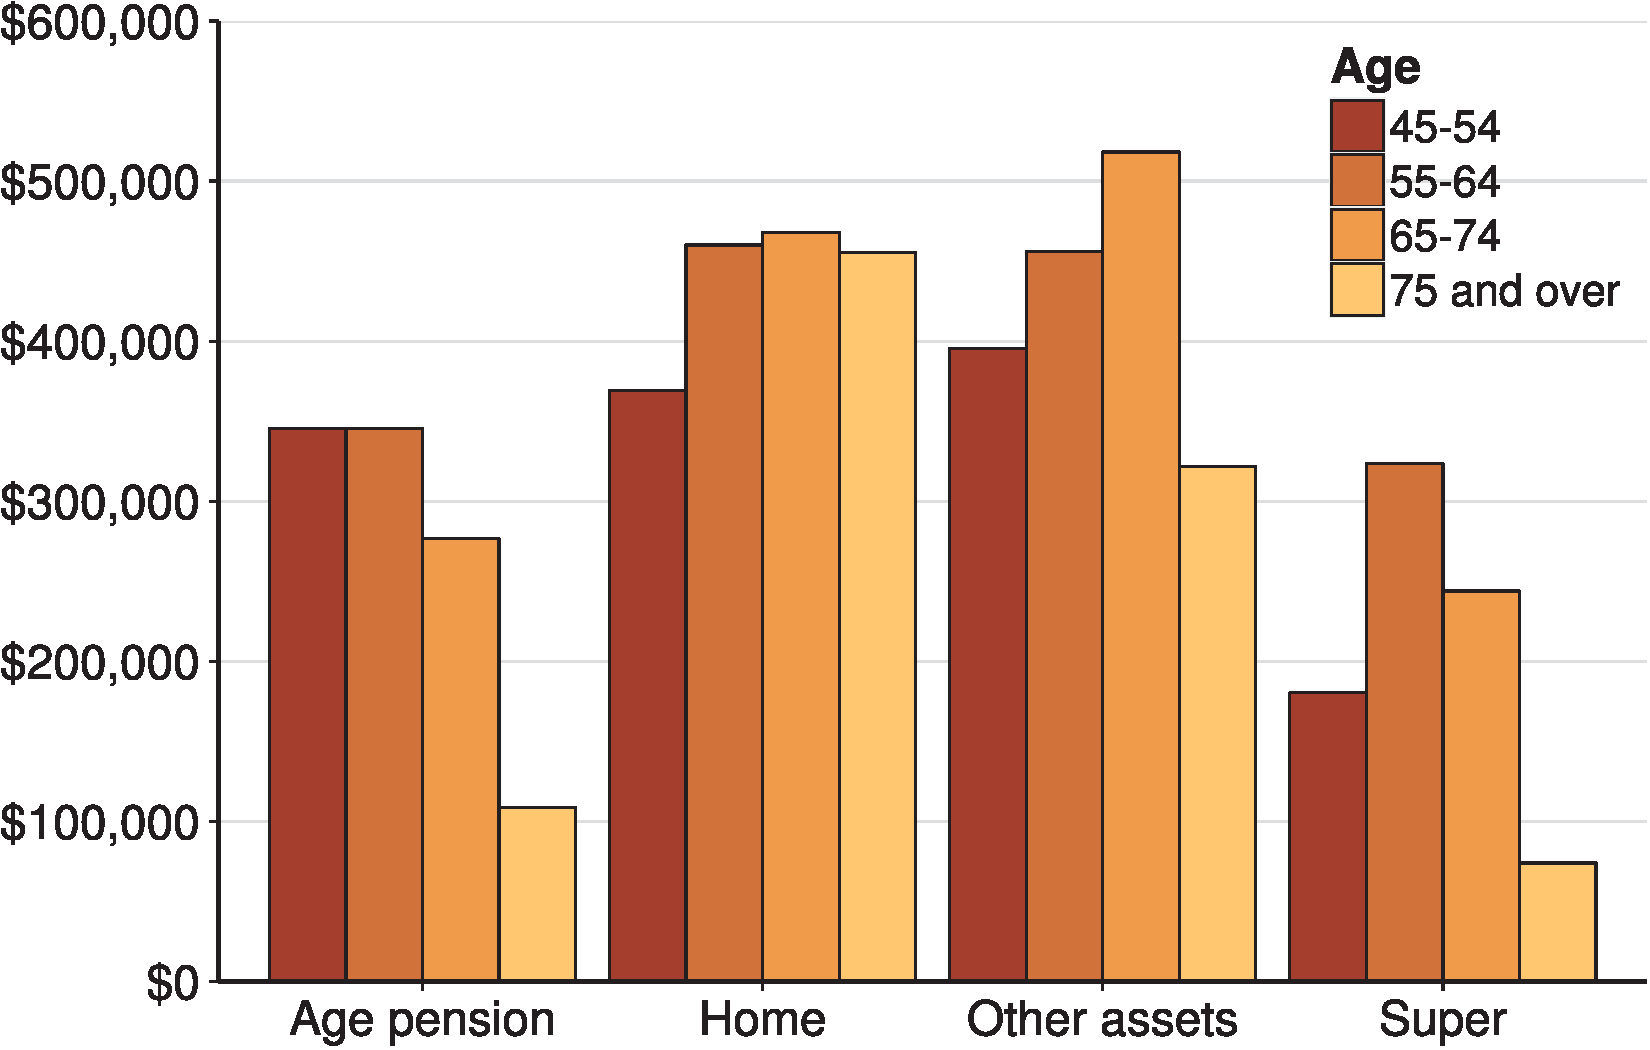
\includegraphics[width=\columnwidth]{super-atlas/Figure2-1-1.pdf}
\fnotes{fig:SUPER-2-1}{Home is net of related mortgage liabilities; other assets are net of other liabilities; superannuation excludes at least some defined benefit schemes. Net present value of Age Pension based on average annual pension payments received by households in each age group in 2011-12, inflated forward to 2013-14. The annual average Age Pension payment is converted into a capital value using a discount rate equal to the Age Pension indexation rate of 4 per cent and an average life expectancy for those aged 65 now of 89 years for women and 86 years for men. The net present value of lifetime Age Pension payment assumes that the average real pension currently received by households in each age group continues to life expectancy. Does not account for future expected increases in private retirement saving before retirement, especially for households aged 45 to 54 years and 55 to 64 years where the bulk of households are not yet retired.}

\source{\gao\ \textcites{ABS2013t}{ABS2015HouseholdIncomeWealth1314}.}
\end{figure}

Many commentators equate retirement savings with superannuation. But superannuation savings (pillars 2 and 3) are the least important part of Australia’s retirement incomes system. While Australians save in a variety of ways, super is only 15 per cent of the wealth of most households (\Vref{fig:SUPER-2-1}). And while homes are a large part of accumulated wealth, households of all ages, incomes and wealth typically have other investments that are greater than their superannuation assets.\footnote{\gao\ \textcites{ABS2015HouseholdIncomeWealth1314}{ABS2013t}}  For older households, assets other than super are often even larger than the value of homes.

These patterns partly reflect the immaturity of the superannuation system.\footnote{%
The Superannuation Guarantee was only introduced in 1992-93, with compulsory contributions rising from 3 per cent of wages in that year to 9 per cent from 2002-03, before reaching the current 9.5 per cent in 2013-14. The Super Guarantee rate will remain fixed at 9.5 per cent until 2021. It will then increase by half a percentage point each year until it reaches 12 per cent. 
} It will be another two decades before typical retirees have been contributing at least 9 per cent of their wages to super for their entire working lives. But even younger generations that have been paying the 9 per cent Superannuation Guarantee since they started work tend to save more outside superannuation.\footnote{For a more detailed analysis of trends in asset holdings by age, see \textcite[][14]{DaleyWoodWeidmannEtAl2014}.}  


As discussed in \Cref{sec:SUPER-3-2}, the fact that Australians save for their retirement through vehicles outside of superannuation has important implications for the amount of superannuation people need for a comfortable retirement. In particular, it is unreasonable to expect superannuation savings alone to fund a comfortable living standard in retirement. Rather, most retired Australians draw on a range of assets to support their retirement – including housing and other investments outside of superannuation. 

Nor will superannuation replace the Age Pension as the most important component of retirement incomes for the vast majority of retirees. The capital annuity value of the average Age Pension payments that households aged 65 years and over can expect to receive over their remaining lives is larger than the average superannuation savings of these households (\Cref{fig:SUPER-2-1}).\footnote{This is consistent with estimates by the \textcite[][7]{ActuariesInstitute2015RetirementIncomes}, which estimates the value of the full rate Age Pension for a people retiring today at the age of 65 at \$816,000 for couples, \$419,000 for a single man and \$482,000 for a single woman – far more than expected average super balances.} The present value of Age Pension payments that will be received by those aged 55 to 64 years and set to retire in the next few years is also larger than the average superannuation savings of these house-holds. 


\section{Superannuation provides several tax breaks}
There are two distinct phases in the tax treatment of superannuation with varying tax treatments for contributions, earnings and payouts, as shown in \Vref{fig:SUPER-2-2}.

\begin{figure}
% \captionsetup{skip=-5pt}
\caption{Tax settings differ across each phase on superannuation\label{fig:SUPER-2-2}}
% 
\includegraphics[page=6,width=\columnwidth]{super-atlas/PPTX.pdf}
\mdfdefinestyle{Accumulation}{%
	linecolor=DarkOrange,linewidth=1pt,%
	skipabove=0pt,skipbelow=0pt,%
	frametitlealignment=\centering,
	frametitlefont=\small\sffamily\color{white},
	frametitlerule=true,%
	innerleftmargin=3.5pt,
	innerrightmargin=3.5pt,
	frametitlebackgroundcolor=DarkOrange,
	innertopmargin=3.5pt
}

\mdfdefinestyle{Benefits}{%
	linecolor=Orange,linewidth=1pt,%
	skipabove=0pt,skipbelow=0pt,%
	frametitlerule=true,%
	frametitlealignment=\centering,
	frametitlefont=\small\sffamily\color{white},
	frametitlebackgroundcolor=Orange,
	innerleftmargin=3.5pt,
	innerrightmargin=3.5pt,
	innertopmargin=3.5pt
}

% manual adjustments for palatino
\begin{minipage}[t]{0.05\columnwidth}
\scriptsize\sffamily
\begin{tabular}[t]{@{}>{\bfseries}p{\linewidth}@{}}
\\[1.925\baselineskip]  % magic for palatino
Contributions \\[13.5\baselineskip]
Earnings \\[5.5\baselineskip]
Withdrawals
\end{tabular}
\end{minipage}
\hfill
\begin{minipage}[t]{0.47\columnwidth}
\begin{mdframed}[style=Accumulation,frametitle=Accumulation]
\scriptsize\sffamily
\begin{tabular}[t]{@{}>{\raggedright}p{\linewidth}@{}b{0pt}@{}}
				Under the Super Guarantee, employers must contribute 9.5\%\ %
				of a person's earnings to their super \\[0.5\baselineskip]
				Individuals can make additional voluntary
				contributions \\[0.5\baselineskip]
				Contributions (up to cap of \$30k or \$35k p.a.)
				are from pre-tax income and taxed at
				concessional rate of 15\% in the fund \\[0.5\baselineskip]
				Further contributions can be made from
				post-tax income (up to cap of \$180k p.a.),
				and are not taxed again in the fund \\[2\baselineskip]
				%
Superannuation funds are invested, earning
returns \\[0.5\baselineskip]
These earnings are taxed at 15\% in the fund
(10\% for capital gains)  \\[2\baselineskip]
Ordinarily, funds cannot be drawn until reaching preservation age (55 years) \\[0.5\baselineskip]
Most payouts become tax-free from\\ age~60 %\\[0\baselineskip]
\end{tabular}
\end{mdframed}
\vspace{5pt}
\end{minipage}
\hfil
\begin{minipage}[t]{0.33\columnwidth}
\begin{mdframed}[style=Benefits,frametitle=Benefits]
\scriptsize\sffamily
\begin{tabular}[t]{@{}b{\linewidth}@{}b{0pt}@{}}
\begin{tabular}[t]{@{}>{\RaggedRight}b{\linewidth}}%
																			Employers and
																			employees can continue
																			to contribute on same
																			basis as in accumulation phase \\[0.5\baselineskip]
																			%
																			Individuals can only make voluntary contributions beyond 
																			age 64 if still in paid work \\[7\baselineskip]
%
Funds continue to earn returns \\[1.5\baselineskip]
Earnings are not taxed \\[3\baselineskip]
%
The super fund pays out from accumulated funds  \\[0.5\baselineskip]
Payouts are not taxed from age 60
\end{tabular} & 
\end{tabular}
\end{mdframed}
\vspace{5pt}
\end{minipage}
\end{figure}

\textbf{Contributions} to an individual’s retirement savings are made to a nominated superannuation fund. Under the Superannuation Guarantee (SG), employers are required to contribute to the retirement savings of their employees by depositing a proportion of their wage (currently 9.5 per cent) into a nominated superannuation fund.\footnote{The self-employed can make contributions directly to their super fund and claim a tax deduction for the tax already paid on that income on their tax returns.} Employers are only required to make SG contributions on the first \$200,000 of employees’ wages.\footnote{The maximum SG contributions an employer is required to make is determined by the maximum super contributions base, currently set at \$203,240 per year, and indexed annually to average weekly ordinary time earnings, \textcite{ATO2015MaxSuperContrBase}.} Some workers also receive a higher proportion of their wages in employer superannuation contributions, where this has been negotiated under a collective agreement.


These ‘pre-tax’ compulsory contributions are taxed at a flat rate of 15~per~cent rather than a person’s marginal income tax rate. Individuals can also make voluntary contributions by salary sacrificing some of their income, again taxed at 15 per cent. Individuals can also make voluntary contributions by salary sacrificing some of their income, again taxed at 15 per cent.%
\footnote{%
This is only possible for people whose employers offer salary sacrifice arrangements, or for self-employed individual who are eligible to claim a tax deduction on their post-tax super contributions. Otherwise, contributions not made through employers are made out of employees’ post-tax income.%
}  

Individuals can also make ‘post-tax’ voluntary contributions to their superannuation fund, financed from post-tax income, up to the annual post-tax contributions cap of \$180,000.  People aged over 65 can only make post-tax contributions if they are still working.\footnote{Those earning over \$300,000 pay 30 per cent tax on their concessional super contributions. The \$30,000 concessional cap for under 50s is indexed to wages; the \$35,000 concessional cap for over 50s is not indexed (\textcite{ATO2015ConcessionalContrCap}).}  Low-income earners also benefit from a matching 50 per cent government co-contribution on the first \$1,000 of post-tax contributions they make each year.\footnote{\textcites{ATO2015SuperCoContr}{ATO2015IncomeThresholdTest} Those earning less than \$35,454 benefit from the full government co-contribution, while those earning between \$35,454 and \$50,454 are eligible for a reduced co-contribution.} Since people have already paid tax on the income that finances these post-tax contributions, no further taxes are levied when they enter the super fund.

\textbf{Earnings} come from contributions, along with compounded earnings from previous years, which are invested by the superannuation fund. In the accumulation phase, earnings are taxed at a flat rate of 15 per cent (10 per cent for capital gains). The effective tax rate on superannuation fund earnings in the investment phase is typically lower – ranging from 7 to 10 per cent depending on the mix of fund investments – after taking into account dividend imputation credits for investments in Australian equities.\footnote{For example, \textcite[][39]{Mercer2015GlobalPensionIndex}  suggests that the net effective tax rate for many super funds in the accumulation phase is around 8~per~cent.}

Once in the benefits phase and aged 60, any earnings on funds in a superannuation account are tax-free. The effective tax rate on superannuation fund earnings in the benefits phase is negative since funds pay no tax on earnings but receive full refunds on any unused dividend imputation credits.\footcites{ATO2015RefundingImputationCredits}[][Appendix~B]{FinancialSystemsInquiry2015} The tax-free status of earnings for retirees dates back to the era when superannuation benefits withdrawn were taxable. Exempting earnings for account-based pensions avoided the double taxation of benefits.\footcite{HenryTaxReview2010} However, since tax on benefits was removed in 2007, this rationale for exempting earnings for retirees no longer applies.%
\footnote{Some commentators have argued that tax-free earnings support encourages people to take their super benefit as an income stream, rather than as a lump sum. However, recent evidence suggests that people already draw down on their assets in an orderly fashion \textcite[][16]{ProductivityCommission2015SuperPolicyPostRetirement}.} 

 \textbf{Payouts} from the accumulated savings in the superannuation fund begin in the benefits phase.  Retirees can only start to withdraw their superannuation ‘benefits’ after reaching the preservation age, currently 55 years of age.\footnote{The preservation age is set to rise from 55 today to 60 by 2024. Some benefits can be accessed prior to preservation age, such as those that accrued prior to 1999, \textcite{ATO2015WhenYouCanAccessYourSuper}.} Benefits can be paid as either an income stream or as a lump sum. Either way, payouts from the account are tax-free from age 60.%
 \footnote{Some superannuation benefits are not tax-free on retirement for over 60s, such as some defined benefit superannuation schemes. In these schemes benefits withdrawn may still be taxable where taxes liable on contributions and fund earnings have not already been paid in the fund. For more detail on the different tax treatment of super fund benefits when withdrawn, see \textcite{ATO2015HowTaxAppliesToSuper} and \textcite[][13]{Mercer2015SubmissionToReThink}.}

\FloatBarrier
 \section{The purposes of superannuation are becoming clearer}
 Despite assets of \$2 trillion,\footcite{APRA2015JuneSuperPerformance} annual administrative and management costs of \$21 billion,\footcite{MinifieSavageCameron2015} and tax breaks on contributions and earnings costing \$25 billion in lost tax revenue each year, ({see \Cref{sec:SUPER-2-8}}) the superannuation system does not have legislated aims. 

It is widely agreed, however, that the system should promote retirement savings so that people enjoy a higher standard of living in retirement, while reducing government’s future Age Pension liabilities, subject to the budgetary costs of doing so. The recent Financial System Inquiry recommended that the contemporary purpose of superannuation should be ‘to provide income in retirement to substitute or supplement the Age Pension.’\footcite[][95]{FinancialSystemsInquiry2015}

 Originally, the superannuation system was set up to achieve at least four objectives:\footcite{Greenwood2010}
 \begin{enumerate}
\item increasing local savings so that Australia was less dependent on foreign capital for economic stability
\item increasing local savings that could be invested in infrastructure
\item encouraging people to save more while they are working so they more to spend in retirement
\item reducing future government liabilities for the Age Pension
 \end{enumerate}

The first of these aims – creating a pool of Australian capital for investment in Australia – is less relevant today. It was conceived in an era that was focused on the ‘twin deficits’ – current account and budget deficits – and the concern that Australia was over-reliant on overseas capital to fund its growth. With the increasing mobility of international capital, it is less clear that this is a real economic problem today. While Australian superannuation funds played a significant role in financing the de-leveraging of corporate Australia during the global financial crisis,\footcites{Henry2009}{RBA2014FinancialSystemInquirySubmission} the Financial System Inquiry argued that ‘funding economic activity is a consequence of a well-designed long-term savings vehicle that invests in the interests of its members, rather than an objective in itself’.\footcite[][98]{FinancialSystemsInquiry2015}

Similarly, it is not clear that greater superannuation balances are required to fund infrastructure. Only a small portion of the existing pool is invested in infrastructure.\footnote{Only 4 per cent of funds managed by APRA-regulated superannuation funds are invested in infrastructure \textcite[][Table~1d]{APRA2015a}.} 
There is no shortage of funds, from both local and overseas investors, for Australian infrastructure assets with proven cash flow.%
\footcite[][188]{ProductivityCommission2013PublicInfrastructure}
Investors are relatively reluctant to support new infrastructure with uncertain returns.\footcite[][131]{ProductivityCommission2013PublicInfrastructure}  However, this reflects the poor risk and return of these investments, illustrated by a number of high profile failures,\footcite[][10]{ElaurantMcDougall2015} rather than any shortage of capital.

Instead the superannuation system today is primarily about \emph{consumption smoothing} – maintaining a more consistent standard of living across people’s lives.\footcite[][288]{MirrleesAdamBesleyEtAl2011} Superannuation encourages people to save while they are working so they have more to spend in retirement.%
\footnote{The superannuation system also aims in pension phase to encourage people to manage financial risks in retirement (\textcite{MaddockKing2015}), an issue beyond this report’s scope.} %
 It is well established that people tend to focus disproportionately on the short term, leading many to save less for their retirement than is required to maintain relatively consistent consumption levels across a lifetime.\footcite[][4]{FinancialSystemsInquiry2015} Although superannuation leads people to save less outside of superannuation than they would otherwise, it leads to higher \emph{total} savings at retirement (including superannuation).\footcites{GruenSoding2011}{Connolly2007}

 Superannuation also requires governments to give up tax revenue today so that governments do not have to spend so much on the Age Pension in future. This encourages intergenerational equity since each generation pays more of the costs of its own retirement, rather than imposing this burden on the next generation. 

 So overall, the superannuation system is designed to promote retirement savings so that people enjoy a higher standard of living in retirement, but with less support from government through the Age Pension, reducing the burden on future taxpayers. 

 However, superannuation does not and should not aim to provide limitless support for savings that increase retirement incomes. We would all like to be rich. But the benefits of higher retirement incomes must be balanced against the costs of achieving them. 

 Similarly, the superannuation system should not seek to replace the Age Pension entirely for all, or even most, retirees. The budgetary cost of doing so would be crippling. The tax breaks would cost the budget much more than the Age Pension. To ensure that a very large number of people didn’t need an Age Pension, tax breaks would need to support \emph{everyone} to save enough to support themselves in retirement beyond average life expectancy even if they don’t live this long. Given targeting would not be perfect, there would be substantial tax breaks beyond those needed to replace the Age Pension for most people. 

 For this reason, the Financial System Inquiry recommended focusing superannuation on providing ‘income in retirement to substitute or supplement the Age Pension.’ Implicitly, superannuation should not aim to support the savings of those who already have such ample resources that they are not going to qualify for even a part Age Pension.%
\footnote{%
Of course, some of those that retire without qualifying for the Age Pension may qualify later in retirement as they draw down on their savings. The level of super savings required for a reasonable retirement, and where taxpayer support might be justified, is discussion in \Cref{sec:SUPER-3-3}.
}
  And implicitly, superannuation should not provide limitless support to savings regardless of the costs to reduce Age Pension liabilities.

\section{Superannuation tax breaks play several roles}\label{sec:SUPER-2-4}
Within this superannuation system, what are superannuation tax breaks supposed to do?

Superannuation tax breaks increase how much people have to spend in retirement from whatever they do save, by reducing the taxes paid on contributions and earnings.\footcite{Keating2015}  

Arguably, superannuation tax breaks also compensate people for being compelled to lock up their savings in superannuation until retirement,\footcite{Hockey2015IGR} although there is no logical way of calculating an appropriate amount of compensation for this or how it might be targeted. 

The ‘value’ of this compensation is very unequally distributed, since high-income earners receive a large tax break (in terms of tax avoided) per dollar of compulsory superannuation contributions, whereas low-income earners receive no compensation. In future low-income earners (below the tax-free threshold) will be penalised for being compelled to save if the Low Income Superannuation Contribution – which refunds the tax paid on compulsory super contributions to those earning less than \$37,000  – is abolished from 2017-18 as currently legislated. Ironically the current system provides the least benefits through tax breaks for compulsory savings to low income earners, even though this group tends to have the greatest preference for immediate consumption rather than saving.\footnote{There is good evidence that higher ability (\ie~higher earning) people are more patient and tend to save more (\textcite[][616--623]{BanksDiamond2010}).} 

\begin{figure}
\captionwithunits{Tax rates on earnings from savings through superannuation are lower than other savings vehicles}%
{Real effective marginal tax rate on long-term savings vehicles, per cent}\label{fig:SUPER-2-3}
% 
\includegraphics[page=7,width=\columnwidth]{super-atlas/PPTX.pdf}
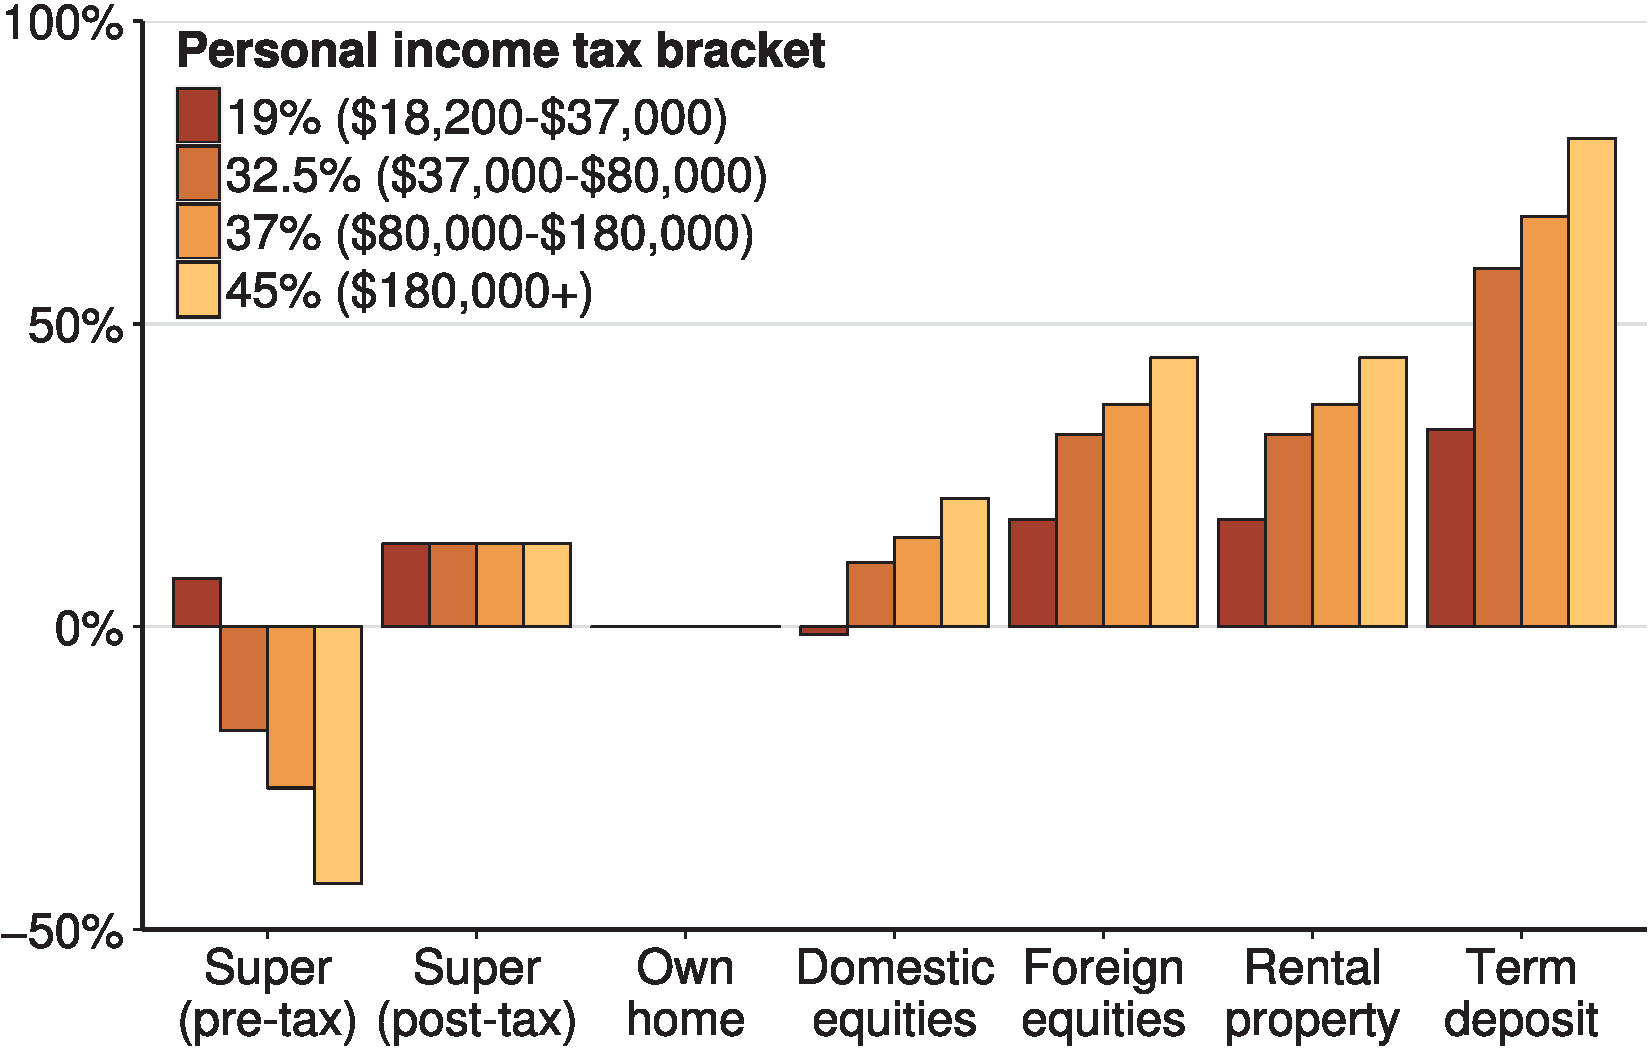
\includegraphics[width=\columnwidth]{super-atlas/Figure2-3-1.pdf}
\fnotes{fig:SUPER-2-3}{%
As explained in \Cref{appendix:SUPER-approaches-measures-for-tax-rates-on-savings}, we define the real effective marginal tax rate on saving as the income foregone due to tax, as a proportion of the pre-tax return (net of inflation). Effective marginal tax rates are presented relative to a pre-paid expenditure tax (\ie~\TEE) benchmark. This approach is consistent with the approach to calculating real effective marginal tax rate rates adopted in the Henry Tax Review. Assumes superannuation earnings are taxed at an average effective rate of 8 per cent in the fund, reflecting the concessional treatment of capital gains (10 per cent tax rate) and dividend imputation for investments in domestic equities. Assumes 6 per cent nominal return; 2.5 per cent inflation; all investments are held for 25 years; for property and equities capital gains tax is only crystallised and paid at the end of 25 years; for property and equities, 50 per cent of the return is attributable to capital gain, 50 per cent to rental or dividend income; dividends on domestic equities are fully franked. Ignores impacts on qualifying for welfare payments. 
}

\source{\textcites{HenryTaxReview2010}[][9]{Wakefield2009} and Grattan analysis.}
\end{figure}

Superannuation tax breaks are also supposed to encourage additional savings, over and above compulsory contributions. The income used to finance superannuation contributions is taxed less, and the earnings on superannuation fund balances are taxed less than other forms of savings, so that the real after-tax returns are better, for a given pre-tax return, than can be achieved through other forms of savings, as shown in \Cref{fig:SUPER-2-3}.%
%
\footnote{%
\Cref{fig:SUPER-2-3} presents the effective marginal tax rates on savings compared to a pre-paid expenditure tax (or \TEE) approach, where tax is paid on the income used to finance savings, but earnings and withdrawals are tax free. Comparing effective tax rates to a \TEE\ approach shows the degree to which taxes on savings result in a bias for or against future consumption. A positive effective tax rate compared to a \TEE\ approach implies a bias against future consumption, whereas a negative effective tax rate implies a bias towards future consumption. This approach is consistent with analysis of effective tax rates on savings contained in the Henry Tax Review and the UK’s Mirrlees Review. 
See \textcites{HenryTaxReview2010}{Wakefield2009}[][322]{MirrleesAdamBesleyEtAl2011}.%
}
%  
Most taxpayers who contribute to superannuation from their earnings before tax have more to spend in retirement than if they had saved their wages after tax, but paid no tax on the returns to their savings. Those that put money into super from pre-tax income just before retirement receive an even larger benefit since they avoid income tax on the money saved, and then benefit from tax-free super earnings and withdrawals once they retire.

\section{Taxes reduce the incentives to save; super tax breaks dampen this effect}\label{sec:SUPER-2-5}
So what is the rationale for tax incentives to save more through superannuation?

When individuals earn income they face a choice between spending it right away, or saving to fund spending, or ‘consumption’, in the future. In theory, rational taxpayers look at how much real earnings on savings will increase their future power to consume. They discount the value of future consumption by applying what economists call a ‘discount rate’, which is a measure of how much they prefer consuming something today rather than tomorrow. 

Taxes on the income from savings reduce the incentives to save.\footcites[][32]{HenryTaxReview2010}[][58]{Treasury2015BudgetPapers201516}[][295]{MirrleesAdamBesleyEtAl2011}  By taxing the returns to saving, income taxes make future consumption more ‘expensive’, since people will have less than otherwise to consume in the future if they save a dollar today. By definition, taxes on savings lead to consumption choices that differ from the choices people would prefer to make in the absence of taxation.\footcite[][295]{MirrleesAdamBesleyEtAl2011} Taxes on savings also reduce the incentives to work today in part to save for the future.\footcite[][12]{HenryTaxReview2010}  


Some commentators have argued that broad superannuation tax breaks are a worthwhile step towards lower taxes on earnings on savings in general.\footcite{CarlingCowanErgas2015}  They argue that all savings income should be tax-exempt to avoid any bias against savings.\footnote{Of course, this logic would only apply to superannuation it if were a full \TEE\ system, with no concessional tax rates on any contributions.} This argument is sometimes buttressed by claims about tax rates on savings that sound extremely high. While these grab headlines, they calculate tax rates on savings in artificial ways that are very different from the way that effective tax rates are typically calculated.  

Australia’s personal income tax system already taxes most returns from long-term savings at a lower rate than other income, or exempts them, consistent with an expenditure tax approach (\Cref{appendix:SUPER-approaches-measures-for-tax-rates-on-savings}).\footcite[][12]{HenryTaxReview2010}  Around 60 per cent of household savings is concentrated in owner-occupied housing and superannuation, where the returns to savings are taxed lightly, or not at all. 

However, it is not obvious that it is bad to tax the earnings from savings. The UK’s Mirrlees tax review concluded that to avoid bias against savings, only the risk free component of investment returns – the ‘return to waiting’ – should be untaxed.\footnote{\textcite[][284]{MirrleesAdamBesleyEtAl2011} However, the authors also acknowledged that some taxation of the normal risk-free return from financial capital investment may be desirable to limit distortions between investments in physical and human capital (p.~311).} 
Other recent analyses have concluded that even the risk-free return to savings should be taxed, albeit at a lower tax rate than other income.\footnote{\textcite{BanksDiamond2010}. The authors point to evidence of a positive correlation between individuals’ earnings capacity and their willingness and ability to smooth consumption over their lifetime by savings, as well as greater uncertainty about lifetime earnings for those with low earning capacity.}  Alternatively, it can be argued that all earnings from savings should be taxed at marginal rates of income tax because savings tend to lead to concentrations of wealth even more unequal than the distribution of income.\footcites{Leigh2013}{Piketty2013}[][23]{Ingles2015}

\phantomsection\label{paragraph:SUPER-progressivity-should-be-transparent}
Even if income taxes on savings were unreasonably high, tax breaks specific to superannuation would be a poor solution to the problem. As the progressivity of the tax system is a basic value choice, changes to the level of progressivity should be made as transparent as possible. The complexity of superannuation tax breaks conceals how they effectively reduce tax rates for a limited set of taxpayers. Such complexity increases the opportunity for well-resourced vested interests to benefit at the cost of the public interest.\footcite{Teles2013}  

\section{Savings outcomes are not affected much by tax rates or incentives}\label{sec:SUPER-2-6}
There is a more fundamental problem with claims that taxes on earnings discourage savings and drag on economic growth. Taxes on savings have limited influence on how much people actually choose to save, particularly people with high incomes. Savings behaviour isn’t just determined by the rate of return to savings after tax. Actual savings are influenced by many factors including:
\begin{enumerate}
\item how much \emph{earnings} on savings increase the amount they have to spend (which is influenced by taxes on earnings)
\item their life circumstances
\item the desire to smooth spending over the life span
\item the desire to leave a legacy
\end{enumerate}

Tax incentives for saving -- such as the superannuation tax breaks -- only affect the first of these drivers. In practice, life circumstances and lifetime consumption smoothing often play a much larger role in savings decisions. High-income earners often want to maintain a lifestyle in retirement similar to that enjoyed while working. Typically this requires much more income than the Age Pension would provide. They are prepared to pay whatever tax is imposed to ensure a high standard of living in retirement. By contrast, those on lower incomes tend to value immediate consumption more than those on higher incomes.\footcite{DynanSkinnerZeldes2004}  

The empirical evidence from around the world confirms that those on higher incomes are more likely to save, and they tend to save about the same amount irrespective of tax rates. Most studies have found that tax incentives for retirement savings have little effect on the total amount saved, as summarised in \Vref{fig:SUPER-2-4}.

\begin{figure}
\captionwithunits{Tax-preferred treatment of voluntary retirement savings encourage relatively little new savings}%
{Percentage of new savings in tax-favoured retirement accounts, by study}\label{fig:SUPER-2-4}
% 
\includegraphics[width=\columnwidth,page=8]{super-atlas/PPTX.pdf}
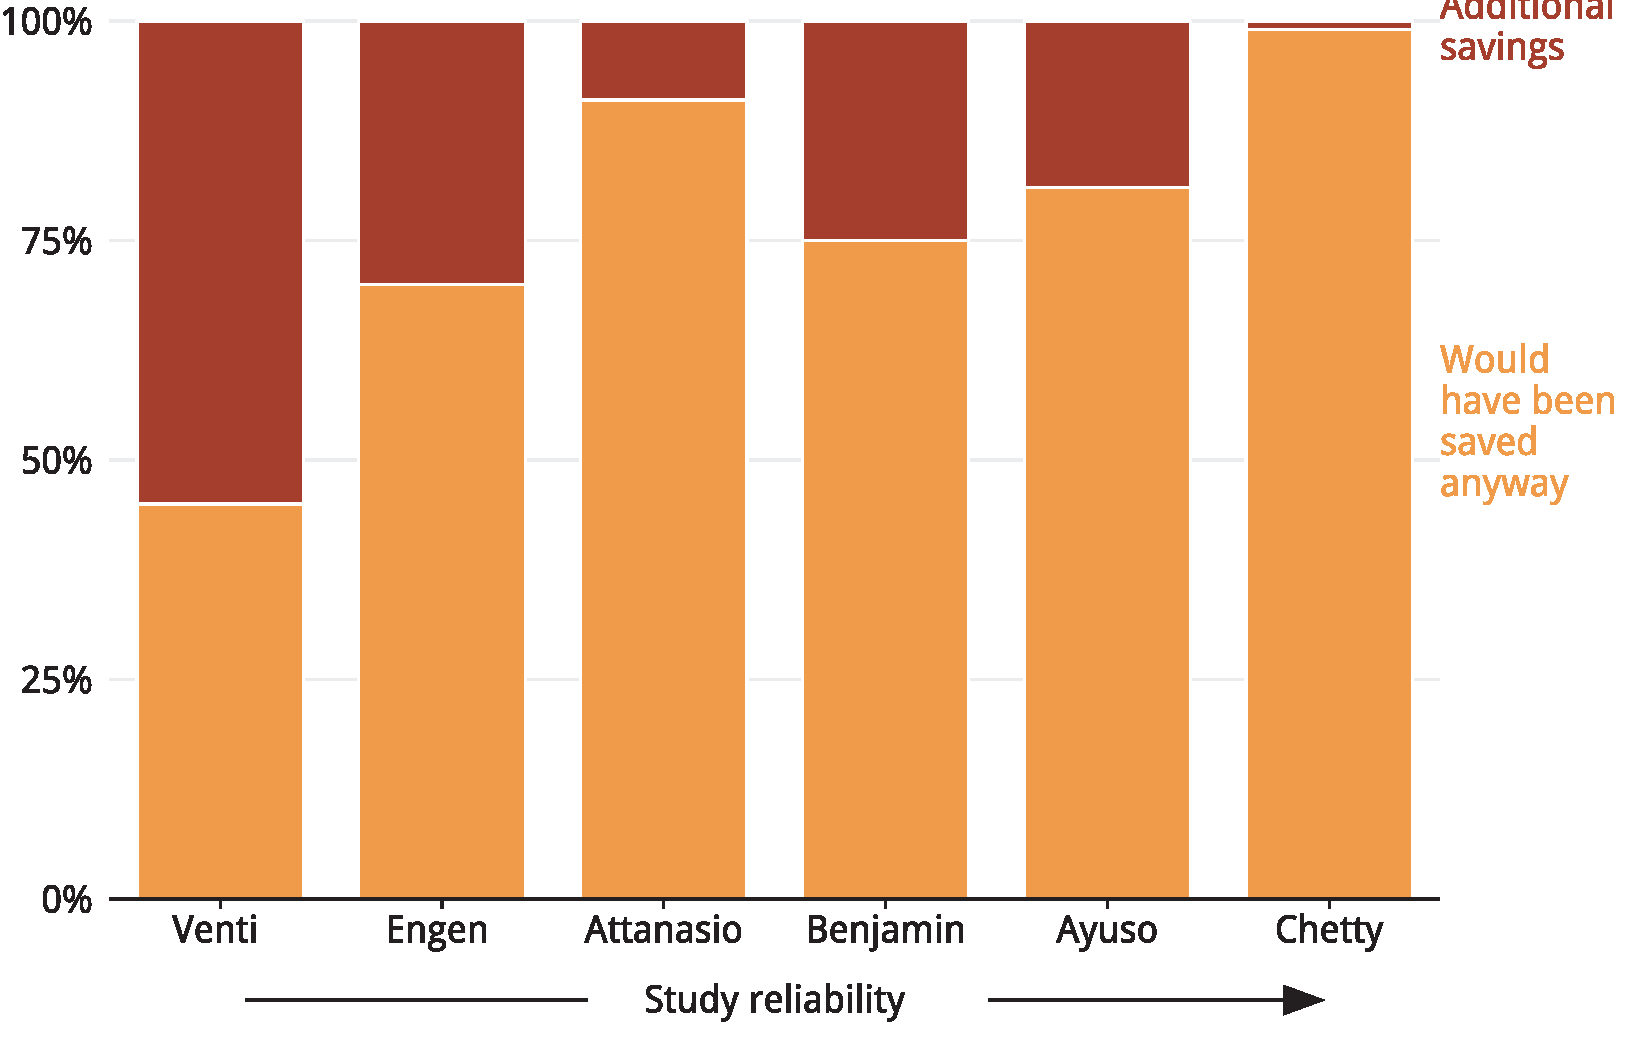
\includegraphics[width=\columnwidth]{super-atlas/Figure2-4-1.pdf}
\notes{Additional savings is new savings from reduced consumption and/or increased labour effort. Of course, if taxes on savings are lower, the ultimate value of those savings will be higher. For Venti we report the mid-point estimate for new savings across a number of studies. For others, we report the maximum estimate for new savings.}

\source{\textcite{PoterbaVentiWise1996} for Venti; \textcites{EngenGale2000}{Benjamin2003}{AttanasioBanksWakefield2004}{AyusoJimenoVillanueva2007}{ChettyFriedmanLethPetersenEtAl2014}}
\end{figure}

However, those with higher incomes, and older savers, tend to switch their savings into whichever investment vehicle pays the least tax.  \textcite{EngenGale2000}, \textcite{AttanasioBanksWakefield2004}, and \textcite{Benjamin2003} all find that tax-advantaged retirement savings accounts have generated limited new savings in the US, with most contributions ‘reshuffled’ from other savings vehicles.\footnote{In contrast, \textcite{PoterbaVentiWise1996} summarizing various studies from Venti and Wise (1985; 1986; 1987; 1990; 1991) find a larger ‘new savings’ effect. 
However, there are a range of data and methodological problems with these studies, particularly, the failure to fully control for difference preferences between participants and non-participants in tax-advantaged savings programs or within these groups over time \textcite{EngenGaleScholz1996} More recent studies in \textcites{Benjamin2003}{EngenGale2000}  have attempted to overcome these issues by using improved data and techniques, and found very little new savings.}    \textcite{AyusoJimenoVillanueva2007} find a similar effect for tax-favoured retirement plans in Spain. 

Tax breaks for savings are more likely to generate additional savings for those on low and middle incomes.\footnote{\textcite{OECD2007EncourageSavingsThroughTaxPreferredAccounts} A review of the experience of tax-preferred savings accounts in 11 OECD member countries suggests that that high-income people are most likely to participate in tax preferred savings plans but tax preferred accounts only create new savings when people of moderate incomes participate in them.}
People in those income categories tend to value future consumption less (that is, they apply higher discount rates),\footcite{DynanSkinnerZeldes2004} the Age Pension is not so much lower than their current consumption, and savings can materially reduce their future entitlements to an Age Pension.\footnote{For example, see \textcite{BlundellEmmersonWafefield2006}. The Age Pension does not discourage many high-income earners from saving, as their assets and income are likely to exclude them from accessing the Age Pension anyway.} 

In contrast, studies suggest that people on higher incomes, and those close to retirement, \textcite{AyusoJimenoVillanueva2007} tend to use tax-advantaged savings programs to reduce the tax paid on money they would save anyway. A detailed study from Denmark showed that reduced subsidies for retirement savings for high-income earners led to almost no reduction in their overall savings efforts.\footnote{\textcite{ChettyFriedmanLethPetersenEtAl2014} is a particularly compelling study because of the quality and size of the data (41 million observations on savings for people from Denmark). Other studies drawing similar conclusions include \textcite{EngenGale2000} and \textcite{Benjamin2003}.}

In Australia, there is only weak evidence that superannuation tax breaks lead to increases in voluntary retirement savings. One recent study concluded that ‘current tax incentives have a limited effect, if any, on the decision to make salary sacrifice arrangements.’\footnote{\textcite{Feng2014} consistent with \Cref{fig:SUPER-A-5}.}
Only about 10 per cent of employees make salary-sacrificed contributions from pre-tax income.\footnote{\textcite{ABS2013t} The proportion of employees making salary sacrifice contributions has fallen sharply, from 50 per cent in 1993, as the Super Guarantee has expanded to cover most workers.}
Tax breaks on superannuation fund earnings may be a strong motivation for those making voluntary post-tax contributions, but many of these contributions appear to reflect tax minimisation strategies rather than additional retirement savings, as noted in \Cref{sec:SUPER-5-1}. The voluntary flow of savings into superannuation does not necessarily mean people are saving more; it merely implies that people are choosing to save in the vehicle that pays the least tax. 

Superannuation has supported higher savings overall, but mostly thanks to compulsory contributions rather than tax incentives to save.\footnote{By definition, superannuation tax breaks boost the post-tax value of compulsory superannuation savings. However, the value of the tax breaks only account for a small portion of the estimated impact of compulsory superannuation on overall household savings.} 
A recent Reserve Bank of Australia study found that each dollar of compulsory superannuation savings added between 70 and 90 cents to total household wealth.\footnote{\textcite{Connolly2007}. That is, there was only a small offsetting fall in other savings in response to the introduction of the compulsory Superannuation Guarantee.} 
At the national level, \textcite{GruenSoding2011} estimate that compulsory superannuation has already boosted private national saving by around 1.5 per cent of GDP, and is expected to rise as the Super Guarantee rises gradually to 12 per cent. And compulsory superannuation savings – unlike the tax concessions – also prompt some individuals to make further voluntary contributions.\footnote{\textcite[][4]{Connolly2007}. Possible drivers of the increase in voluntary savings include greater awareness of the importance of retirement savings due to compulsory super, and the added convenience of making voluntary contributions into accounts already set up to receive compulsory contributions.}

These findings suggest that any tax breaks on savings should be targeted towards low- and middle-income earners, where they will have the most impact on voluntary retirement savings relative to the budgetary cost. Unfortunately, Australia’s current system does the opposite, offering tax breaks on savings that provide the most benefit to high-income earners and are little-used by low- and middle-income earners. 

\section{\mbox{The benefits of super tax breaks must be balanced against the costs}\label{sec:SUPER-2-7}}
Thus the welfare and efficiency losses from taxes on savings must be balanced against the alternatives. All taxes reduce someone’s welfare – they distort decisions away from what people would otherwise prefer. Most taxes also reduce efficiency – they reduce the total amount of economic activity. Those seeking to justify super tax breaks need to show that they provide larger benefits in economic efficiency and welfare than the cost of additional taxes elsewhere to make up the shortfall.

Arguably, the fact that people tend to save almost the same amount irrespective of the tax rate on savings means that savings should be taxed more.\footcite[][21]{Ingles2015}  From an economic perspective, taxes are generally considered to be more efficient if they affect behaviour less in practice than other taxes.

\section{Current superannuation tax breaks are costly}\label{sec:SUPER-2-8}
Superannuation tax breaks are a large and growing cost to the budget bottom line, and other taxes must be higher than otherwise to compensate. The annual revenue lost in superannuation tax breaks – after accounting for potential behaviour change and the interaction between contributions and earnings tax breaks – is over \$25 billion.%
%\footnote{\gao\ \textcites{APRA2014}{APRA2015JuneSuperPerformance}{Treasury2015TES2014}. The combined value of tax expenditures on superannuation contributions and fund earnings using the Treasury’s ‘revenue gain’ approach exceeded \$27 billion in 2014-15, and is expected to rise to \$40 billion by 2017-18 \textcite{Treasury2015TES2014}. It is often cautioned that one cannot simply add together the Treasury’s ‘revenue foregone’ tax expenditure estimates for contributions and earnings tax breaks into one figure. However, we estimate the degree of ‘double counting’ in combining the ‘revenue gain’ tax expenditure estimates from abolishing each of these tax breaks at less than \$1 billion a year over that period. Alternatively, \textcite[][28]{ASFA2015TreasurySubmission} puts the combined annual revenue cost of contributions and earnings tax breaks at \$23 billion in 2014-15.}\label{fn:81} 
\endnote{\gao\ \textcites{APRA2014}{APRA2015JuneSuperPerformance}{Treasury2015TES2014}. The combined value of tax expenditures on superannuation contributions and fund earnings using the Treasury’s ‘revenue gain’ approach exceeded \$27 billion in 2014-15, and is expected to rise to \$40 billion by 2017-18 \textcite{Treasury2015TES2014}. It is often cautioned that one cannot simply add together the Treasury’s ‘revenue foregone’ tax expenditure estimates for contributions and earnings tax breaks into one figure. However, we estimate the degree of ‘double counting’ in combining the ‘revenue gain’ tax expenditure estimates from abolishing each of these tax breaks at less than \$1 billion a year over that period. Alternatively, \textcite[][28]{ASFA2015TreasurySubmission} puts the combined annual revenue cost of contributions and earnings tax breaks at \$23 billion in 2014-15.}\label{endnote:81}
This is well more than 10 per cent of personal income tax collections, which raised around \$177 billion in 2014-15.\footcite[][4--14]{Treasury2015BudgetPapers201516}

The leakage from the personal income tax base will increase, because the costs of superannuation tax breaks are growing much faster than the economy and tax collections. 
In 2015-16 superannuation tax breaks will cost almost \$30 billion in foregone revenue, rising to close to \$40 billion by 2017-18.\footnote{See endnote~\ref{endnote:81}.}

\begin{figure}
\captionwithunits{Superannuation tax breaks are set to increase rapidly}%
{Revenue cost of superannuation tax breaks (2014-15 dollars)}\label{fig:SUPER-2-5}
% 
\includegraphics[width=\columnwidth,page=9]{super-atlas/PPTX.pdf}
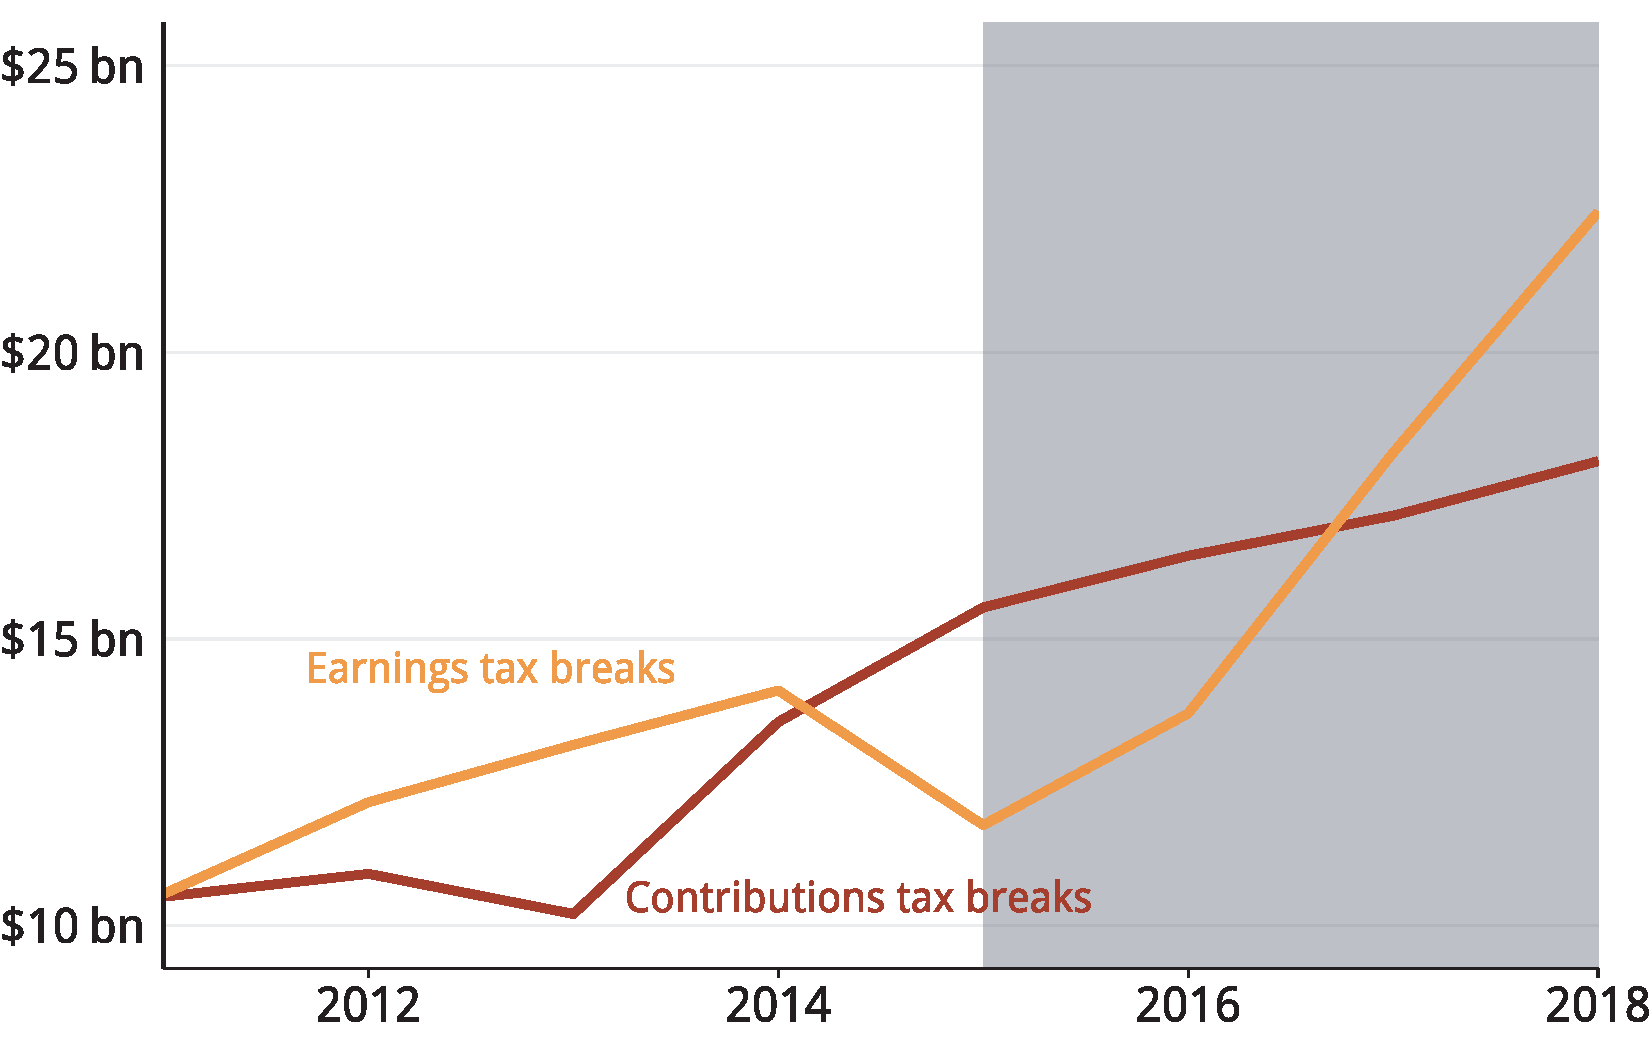
\includegraphics[width=\columnwidth]{super-atlas/Figure2-5-1.pdf}
\fnotes{fig:SUPER-2-5}{Dates are financial year ending. Revenue cost of superannuation tax breaks are estimated relative to an income tax benchmark – they compare tax actually paid with the tax that would be paid if the same contributions and earnings were taxed at each individual’s marginal tax rates, including relevant tax offsets where available. The estimates are based on Treasury’s ‘revenue gain’ approach to estimating tax expenditures and account for behavioural change. See endnote~\ref{endnote:81}.}

\source{\textcite{TreasuryTESvariousyears}.}
\end{figure}

The cost of contributions tax breaks is expected to continue to grow a little faster than nominal GDP, at 4 per cent per year, rising to \textbf{\$18.1~billion} in 2017-18 (\Vref{fig:SUPER-2-5}).\footcite[][4--14]{Treasury2015BudgetPapers201516}  
This reflects both wages growth, population increase, and the fact that 60 to 69 year olds, who tend to make larger voluntary pre-tax contributions to superannuation (\Vref{fig:SUPER-A-7}), will make up an increasing share of the population. 

Tax breaks on earnings are expected to grow much faster at 23 per cent per year, rising to \textbf{\$22.5 billion} in 2017-18. Inherently earnings (and therefore tax breaks on earnings) tend to grow in line with the pool of superannuation assets – driven by new contributions, earnings on balances, less withdrawals. Total superannuation assets have more than doubled in the last 8 years.\footcite[Table~7]{APRA2014}  
In addition, the revenue from taxes and the cost of tax breaks on fund earnings are expected to grow faster than the pool of assets as superannuation funds use up tax losses accumulated during the global financial crisis and carried forward. Tax breaks on earnings are also expected to grow faster than the pool of assets as a greater proportion of the pool comes to be held by those over 60 in pension phase, who pay no tax on superannuation earnings.\footnote{\textcite[][23]{RiceWarner2015SubmissionTaxWhitePaper} projects that the share of superannuation assets held in (tax-free) retirement pensions will rise from 32 per cent in 2014 to 38 per cent in 2029.}  

These trends are likely to continue into the future. In addition, the government is planning to raise the Super Guarantee contribution rate to 12 per cent between 2021 and 2026. This will further increase the costs of tax breaks to the budget as the level of funds channelled into the superannuation system rises.%
\footnote{For example, Treasury analysis undertaken for the \textcite[][13]{CooperReview2013} estimated that the revenue foregone from superannuation tax breaks as a result of moving to a 12 per cent Superannuation Guarantee would exceed the budgetary savings from lower Age Pension spending by close to 0.5 per cent of GDP a year in the short-term, with the net budget cost only falling to 0.2 per cent of GDP a year by 2050. Based on these figures, the cumulative increase in Commonwealth public debt from increasing the Superannuation Guarantee to 12 per cent would exceed 10 per cent of GDP by 2050.} 

There has been extensive commentary about how changes to the tax breaks will have less budgetary impact than the tax expenditure estimates suggest.\footcites{Clare2015}{ASFA2015TreasurySubmission}{Mercer2013a}{Carling2015} However, Treasury’s ‘revenue gain’ tax expenditure estimates cited in this report already account for behavioural change, whereby some people would put less into superannuation and more into other vehicles where they pay less tax than their marginal rate of income tax. 

\begin{smallbox}[tp]{Measuring the value and cost of super tax breaks}{box:SUPER-super-tax-breaks}
Superannuation tax breaks mean that less tax is paid on money saved into superannuation, and less tax is paid on the earnings, compared to if that money was saved outside of superannuation. In this report, the value of superannuation tax breaks, and their distribution among taxpayers, are measured against a comprehensive income tax (or ‘\TTE’) benchmark. Treasury estimates the ‘tax expenditures’ from super tax breaks by comparing the tax paid on contributions and earnings against the tax payable if they were taxed at marginal rates of income tax (\textcite{Treasury2015TES2014}). 

As noted in \Cref{sec:SUPER-what-this-report-does-not-do}, some commentators argue that an expenditure tax approach – where no tax is paid on income from savings – is a desirable structural feature of the tax system, and so the cost of super tax breaks should be measured against such a benchmark. However, arguments about the best policy for taxing savings should not be confused with questions about how to measure their cost (\textcite{DaleyWoodCoates2015}). The income tax benchmark remains the best measure of how much tax breaks cost. Absent superannuation, savings would be taxed under this regime. Of course there are tax breaks for other forms of savings, and these should be measured against the same benchmark. 

Treasury now also estimates the ‘revenue gain’ from abolishing super tax breaks, which takes into account behavioural change. If superannuation tax breaks were abolished, some people would move super savings into vehicles that pay less tax than the benchmark marginal income tax rates. However, the revenue loss from contributions tax breaks is largely unaffected by behaviour change: there aren’t many ways outside of superannuation for taxpayers to reduce the tax payable on the principal invested. 
\end{smallbox}

In any case, behavioural change does not make much difference, particularly for contributions tax breaks.\footnote{\textcite[][124]{Treasury2015TES2014}. Treasury’s ‘revenue gain’ estimate from abolishing contributions tax concessions assumes that all voluntary super contributions are directed towards other alternative tax-preferred investments, which are typically funded out of post-tax income. The estimate for earnings tax breaks accounts for lower contributions to super as it becomes a less attractive savings vehicle, and greater voluntary withdrawals from super in order to take advantage of tax-free thresholds and offsets available elsewhere in the personal income tax system.}  
Alternative savings vehicles are much less generous than superannuation. Unlike other savings vehicles, superannuation allows saving from pre-tax income (less 15 per cent), and imposes much lower tax rates (see \Cref{fig:SUPER-2-3}). 

Some commentators argue that an income tax benchmark is not appropriate for measuring savings tax breaks.\footcites{Carling2015}{Sloan2015} They prefer the ‘pre-paid’ expenditure tax benchmark, where earnings and benefits are untaxed but contributions are fully taxed at marginal tax rates (\Cref{appendix:SUPER-approaches-measures-for-tax-rates-on-savings}). Unsurprisingly, the superannuation industry prefers this benchmark, which reduces the apparent size of the tax expenditures. 

However, this benchmark does not reflect the trade-off faced by most people. Only a small proportion of the assets in super are owned by people legally entitled to pay no tax on the earnings of their savings outside of super. 

Under a pre-paid expenditure tax benchmark, Treasury estimated that contributions tax breaks cost \$16 billion in foregone revenue while the earnings regime provides a gain to the budget of \$5.8~billion (\textcite{Treasury2014TES2013}). These estimates show that Australia’s superannuation tax breaks cost \$10 billion more in foregone tax revenue than if Australia adopted an \EET\ system for taxing superannuation savings, which is widely recognised as an amply generous tax treatment for taxing retirement savings.\footcites{MaddockKing2015}{Freebairn2015}

More recently, some have noted that the tax expenditure measures do not account for the additional costs of higher Age Pensions in future if the rules are changed.\footcites[][5--6]{Mercer2013a}[][13--14]{FSC2015}[][3]{Clare2015}
However, the changes proposed in this report will have little impact on Age Pensions, as they are targeted at those who are unlikely to qualify for much Age Pension anyway.%
\footnote{Half the value of super earnings tax breaks go to those in top 20 per cent of income earners (vide \Cref{sec:SUPER-6-2} {infra}).  \Vref{fig:SUPER-3-9} shows that people in the top 10 per cent of income earners are unlikely to receive much Age Pension over their lifetimes, particularly compared to the value of tax breaks they will receive.}  



\chapter{The targeting of superannuation tax breaks overall}
Superannuation tax breaks, as currently structured, are an unfair and costly way to promote retirement savings. By value, most of the superannuation tax breaks go to people on higher incomes. 

In practice these people are likely to save enough, even without superannuation tax breaks, so that they are unlikely to qualify for a part Age Pension. The top 20 per cent of income earners at age 55 have usually already acquired assets approaching \$2 million. Usually they hold more financial assets outside of superannuation than within it. The wealthiest 20 per cent of households headed by someone over the age of 65 have typically saved enough to generate a substantial retirement income: 70 per cent of them have annual incomes over \$50,000, excluding the Age Pension.

Those consistently earning more than \$115,000 a year are likely to save enough just through compulsory superannuation contributions to enjoy an affluent retirement. Their disposable income in retirement is likely to be higher than that of most Australians during their working life. They are likely to have a superannuation balance large enough to disqualify them for the Age Pension for most, if not all, of their retirement years. 

Thus superannuation tax breaks for those consistently earning more than \$115,000 are not required to reduce Age Pension liabilities. Nor can they be justified on the alternative grounds that they compensate for high tax rates on high-income earners.

Incomes tend to be fairly consistent. So those with high incomes in any given year are likely to have high lifetime incomes. Consequently, it is fair enough to target superannuation tax breaks on the basis of annual incomes and contributions.

\section{Superannuation tax breaks primarily benefit high-income earners}
Superannuation provides much larger tax concessions per person to high-income earners. Over half of the value of superannuation tax breaks – for earnings and contributions combined – flow to the top 20~per cent of income earners (\Vref{fig:SUPER-3-1}). \oneraggedpage

\begin{figure}[hbp]
\captionwithunits{Superannuation tax breaks primarily benefit high-income earners}%
{Percentage of values of superannuation concessions per income decile}\label{fig:SUPER-3-1}
% 
\includegraphics[width=\columnwidth,page=10]{super-atlas/PPTX.pdf}
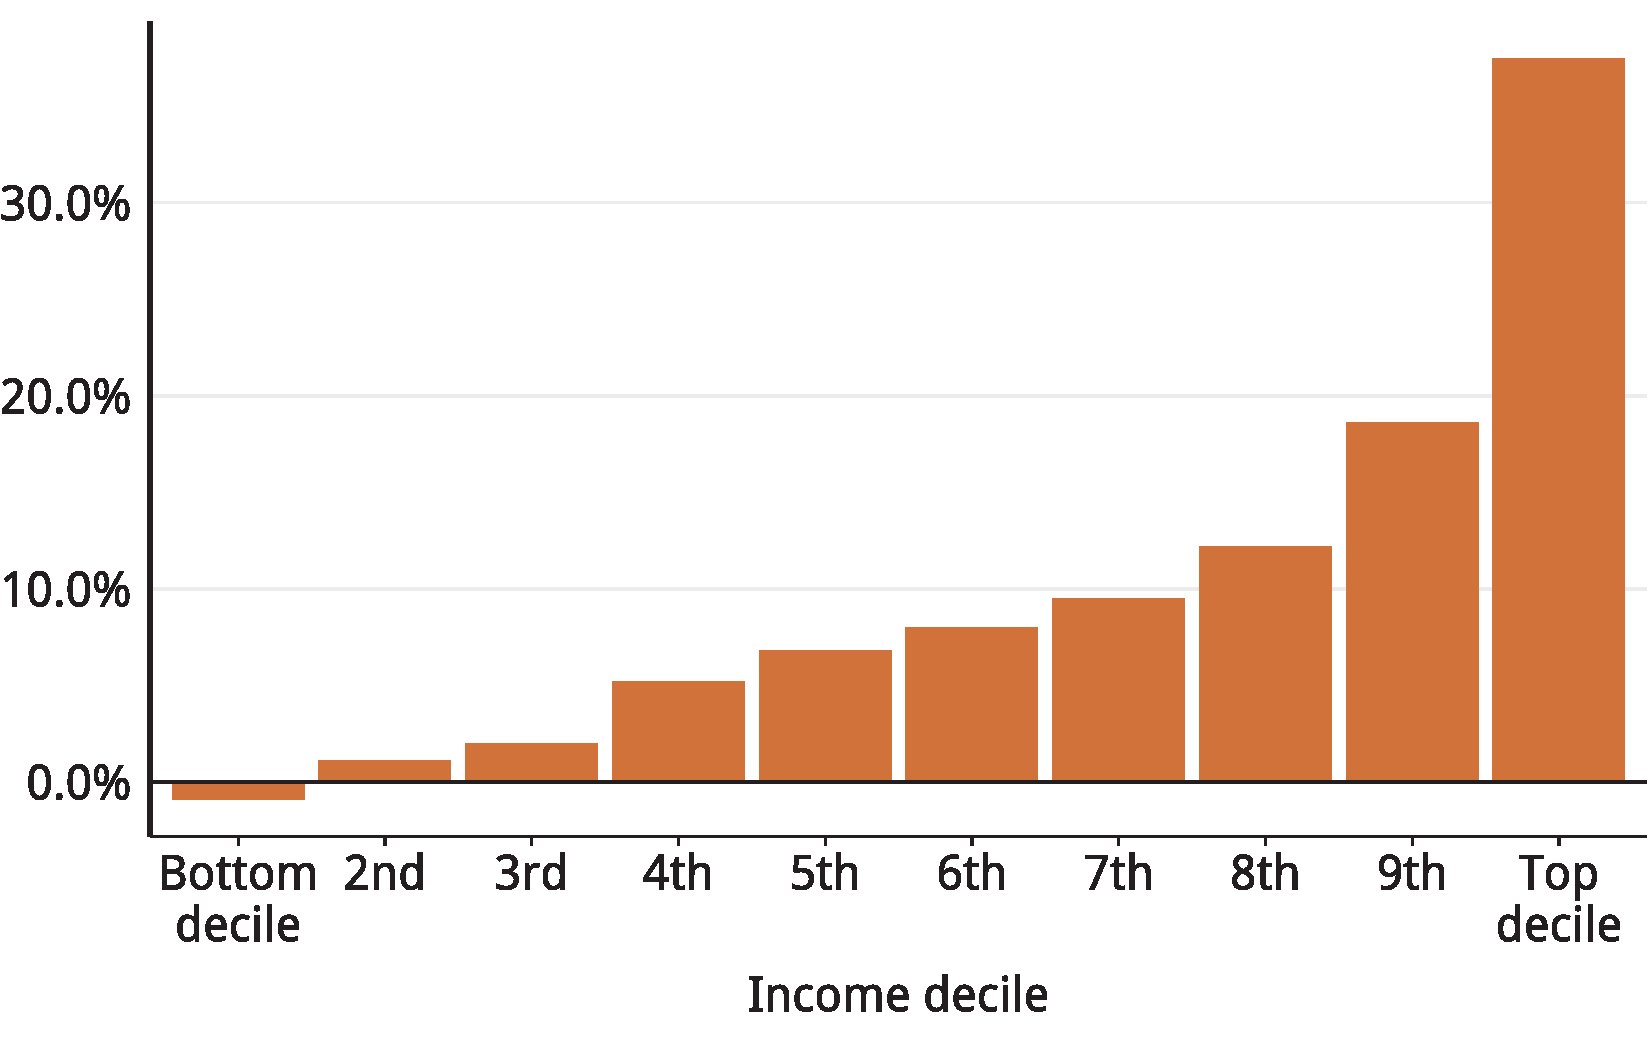
\includegraphics[width=\columnwidth]{super-atlas/Figure3-1-1.pdf}
\notes{The value of tax break is calculated against a comprehensive income tax benchmark, as per \Cref{box:SUPER-super-tax-breaks}; income deciles sorted by taxable incomes for 2011\nobreakdash-12; only includes taxpayers that made a pre-tax contribution in that year.}

\source{\textcite[][138]{FinancialSystemsInquiry2015}.}
\end{figure}

\section{High-income earners are likely to save without superannuation tax concessions}\label{sec:SUPER-3-2}
These high-income earners receiving most of the superannuation tax concessions are likely to save and self-fund their retirement even without government incentives to do so. Few households that have been earning over \$100,000 a year plan to retire onto an Age Pension paying at most \$34,000 a year.\footnote{Combined couple rate of Age Pension, including Maximum Pension Supplement and Energy Supplement (\textcite{DHS2015IncomeTestForPensions}.}  As shown by the savings tax literature discussed in \Cref{sec:SUPER-2-6}, higher income households around the world typically save a substantial portion of their income, irrespective of the tax rates on savings. 

The actual behaviour of high-income households in Australia bears this out. They tend to save substantially in the decade or so before retirement. Wealthy retirees usually earn more from investments outside of superannuation than inside. 



High-income Australians approaching retirement have typically saved substantial assets (\Vref{fig:SUPER-3-2}). Households aged over 50 earning more than \$100,000 a year have amassed average net assets worth more than \$1.7 million. Excluding owner-occupied housing, more than half of these assets are invested outside of superannuation. This suggests that many would save even if there were no superannuation tax concessions. This investment pattern is typical for households of all ages and incomes (\Cref{sec:SUPER-Super-savings-are-least-important-pillar}).

The savings of high-income households before retirement is reflected in their sources of income in retirement. The wealthiest retired households typically earn more from superannuation than less wealthy households (\Vref{fig:SUPER-3-3}). But they also typically earn even more from other investments, suggesting they would have saved for retirement regardless.

% \begin{figure*}
% \begin{minipage}{\columnwidth}
% \captionwithunits{Wealthier retirees earn more from superannuation -- and even more elsewhere}%
% {Average income of retirees in 2009-10, by source}\label{fig:SUPER-3-3}
% \includegraphics[width=\columnwidth,page=12]{super-atlas/newPPTX.pdf}
% \end{minipage}
% \begin{minipage}{\columnwidth}
% \captionwithunits{Most wealthy retirees have annual incomes above \$50,000, mostly from sources outside superannuation}%
% {Average income of the wealthiest 20\%\ of retirees, by source}\label{fig:SUPER-3-4}
% \includegraphics[width=\columnwidth,page=13]{super-atlas/newPPTX.pdf}
% \end{minipage}
% \notes{`Superannuation' includes other private pensions, which account for only a small share of income across all households.}

% \source{\gao\ \textcite{HILDA2015}}
% \end{figure*}

\begin{figure}[p]
\begin{leftfullpage}
\captionwithunits{Wealthier retirees earn more from superannuation -- and even more elsewhere}%
{Average income of retirees in 2009-10, by source}\label{fig:SUPER-3-3}
% \includegraphics[width=\columnwidth,page=12]{super-atlas/newPPTX.pdf}
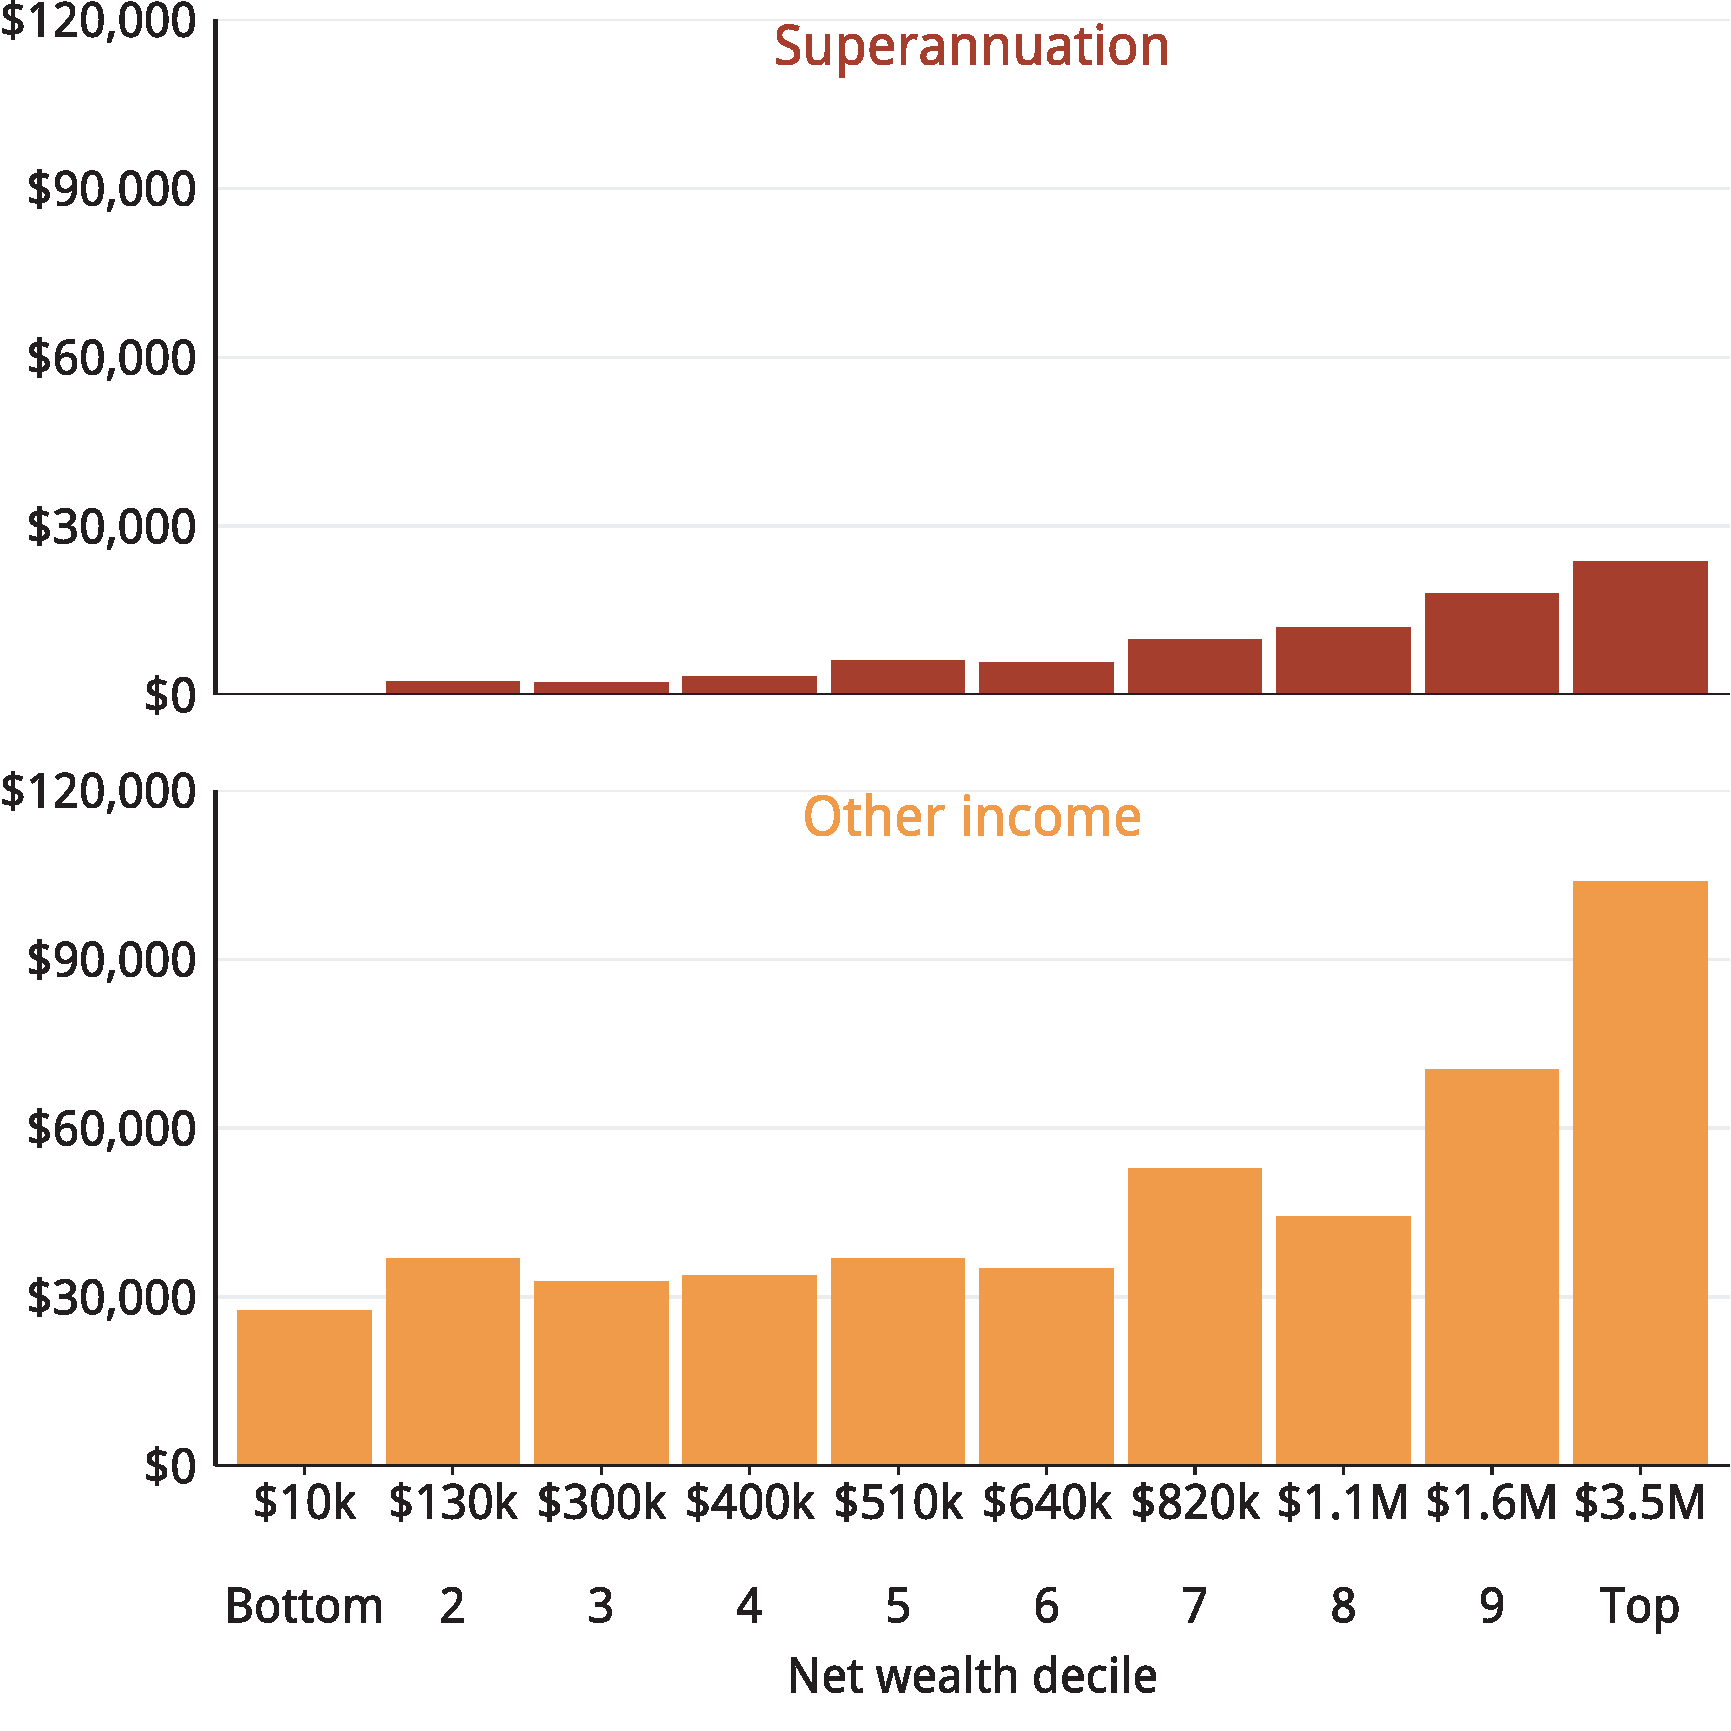
\includegraphics[width=\linewidth]{b5-super-atlas/Figure3-3-1.pdf}
\notes{`Superannuation' includes other private pensions, which account for only a small share of income across all households.}

\source{\gao\ \textcite{HILDA2015}}
\end{leftfullpage}
\end{figure}
\begin{figure}[p]
\begin{fullpage}
\captionwithunits{Most wealthy retirees have annual incomes above \$50,000, mostly from sources outside superannuation}%
{Average income of the wealthiest 20\%\ of retirees, by source}\label{fig:SUPER-3-4}
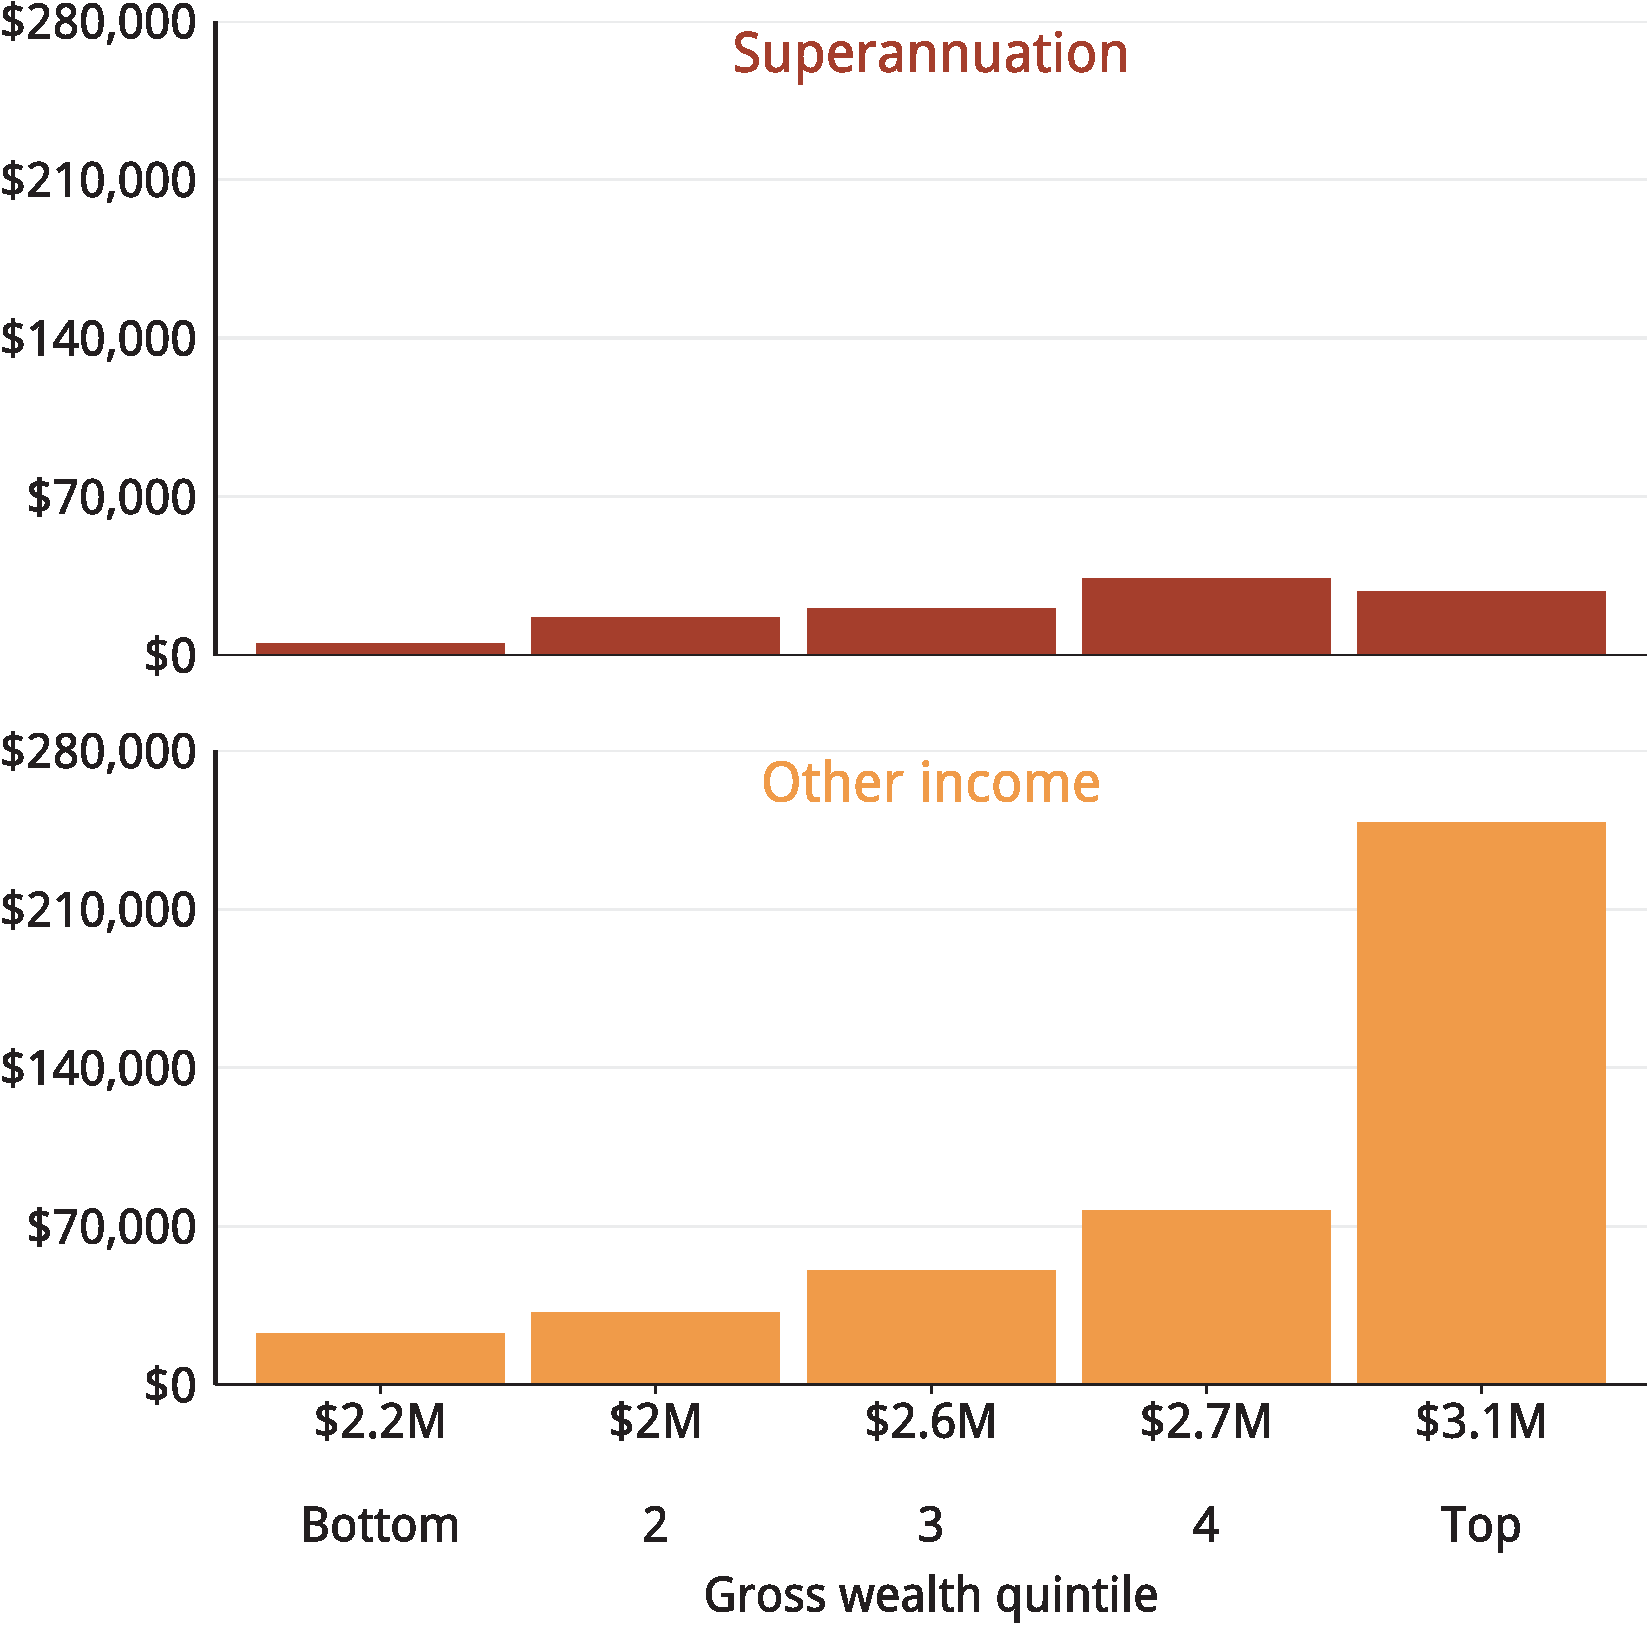
\includegraphics[width=\linewidth]{b5-super-atlas/Figure3-4-1.pdf}
\notes{`Superannuation' includes other private pensions, which account for only a small share of income across all households.}

\source{\gao\ \textcite{HILDA2015}}
\end{fullpage}
\end{figure}

There are not many exceptions. Of the wealthiest 20 per cent of retired households, 70 per cent have annual incomes over \$50,000 (\Vref{fig:SUPER-3-4}). Most of this income is from sources other than the Age Pension and superannuation. 

These patterns may change a little as the superannuation system matures, so that retired households earn more from superannuation than at present. However, it is likely that households of all ages will continue to invest more outside of superannuation than inside (\Vref{fig:SUPER-2-1}). And high-income households are likely to continue to amass wealth to fund their own retirement, irrespective of the superannuation tax incentives.

\begin{figure}
\captionwithunits{Households approaching retirement than earn more than \$100,000 typically build significant wealth outside of superannuation}%
{Average wealth of households earning more than \$100,000 annually, (2011\nobreakdash-12 dollars)}\label{fig:SUPER-3-2}
% 
\includegraphics[width=\columnwidth,page=11]{super-atlas/PPTX.pdf}
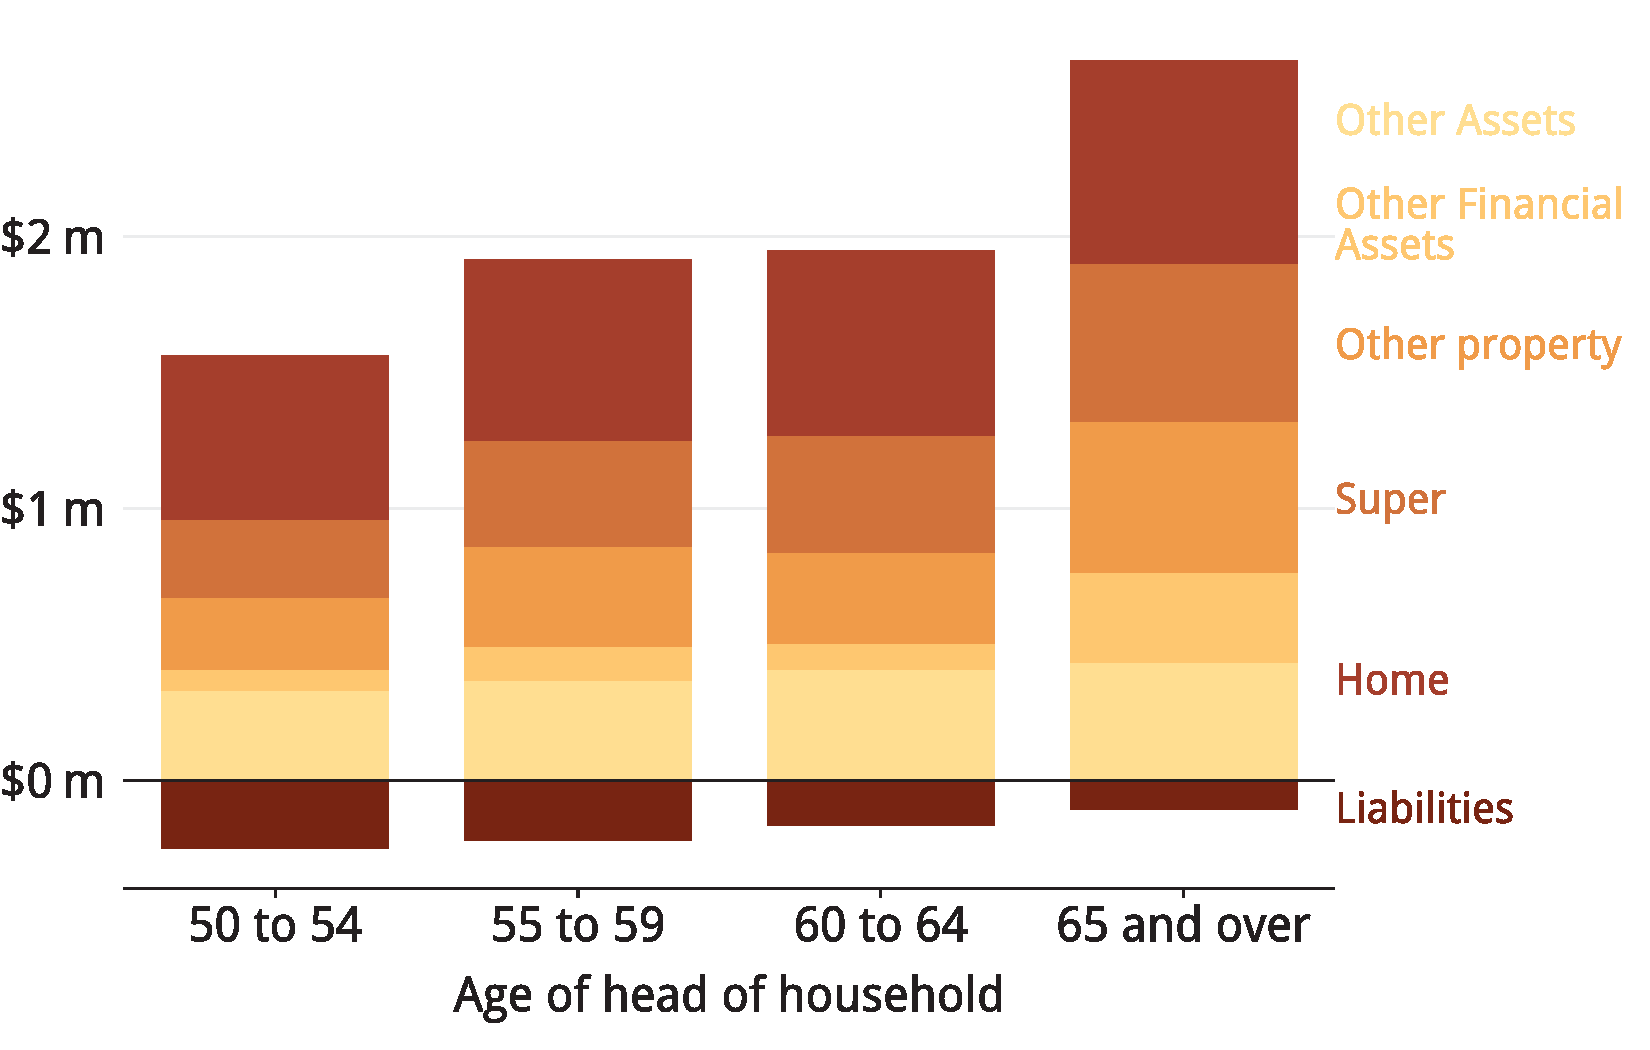
\includegraphics[width=\linewidth]{b5-super-atlas/Figure3-2-1.pdf}
\fnotes{fig:SUPER-3-2}{‘Super’ assets include any interests in both APRA regulated and self-managed superannuation funds. May exclude interests in some defined benefit schemes. ‘All other wealth’ includes other non-financial assets such as the value of vehicles and home contents.}

\source{\textcite{ABS2013t}; Grattan analysis}
\end{figure}

\section{Those earning over \$115,000 a year are likely to enjoy a comfortable retirement without an Age Pension}\label{sec:SUPER-3-3}
At what level of income are people likely to self-fund their retirement through superannuation and other forms of saving? Our analysis shows that people who consistently have taxable income of \$115,000 per year are likely to largely self-fund their retirement through their compulsory superannuation contributions alone. Such people are earning 1.5 times average full time weekly earnings and are in the top 8 per cent of income earners.\footnote{\gao\ \textcites{ATO2015SampleFile1213}{ABS2013AWE}.} Their superannuation savings, together with private savings outside of superannuation, would probably give them sufficient assets that they would not qualify for a part-rate Age Pension for much or all of their retirement. The income from their superannuation savings, together with some drawdown, would fund a lifestyle in retirement more affluent than that enjoyed by over half of Australians before retirement, and by more than two thirds of Australians after retirement. In practice, people with superannuation savings of that size are likely to have even more invested outside of superannuation, and will therefore enjoy even higher incomes in retirement.

A person earning \$115,000 a year would make compulsory superannuation contributions of \$11,000 each year (indexed for inflation). This should generate a superannuation balance of about \$588,000 (in 2015 terms\DEVIATION{}) after 30 years (\Vref{tbl:SUPER-1}). With some superannuation accumulated by a second-income earner, and savings outside super (beyond the family home), a couple would be likely to amass combined assets well over \$805,025. On these assets, retiring homeowner households would not be eligible for a part Age Pension after 2017 (\Vref{tbl:SUPER-2}). Whether they ever qualify for a part Age Pension will depend on the earnings on their assets, and how much they choose to consume in retirement.%
\footnote{Just under 20 per cent of retirees currently aged 80 and over remain self-funded (\ie~don’t draw any Age Pension), compared to 35 per cent of those aged 65 years 
\textcite[][47]{ActuariesInstitute2015RetirementIncomes}.} 

\afterpage{%
\begin{table}
\begin{minipage}[t][\textheight][t]{1.01\linewidth}
\captionsetup{margin = {-3.5em,-1em}, format=hang}
\caption{Account balances (2015-16 dollars) from contributing \$11,000 (indexed)\,p.a.\label{tbl:SUPER-1}}
\begin{tabularx}{\columnwidth}{>{\raggedright}p{0.185\columnwidth}>{\raggedleft}p{0.18\columnwidth}RR}
\toprule
\tblHeadL{Number of years of contributions} & \tblHeadR{Balance accumulated} & \tblHeadR{\%\ of lump sum for a `comfortable' lifestyle} & \tblHeadR{\%\ of lump sum for a `modest' lifestyle} \\
\midrule
$5$ & \$$53$,$218$ & $10$ & $106$ \\
$10$ & \$$120$,$113$ & $22$ & $240$ \\
$20$ & \$$306$,$618$ & $56$ & $613$ \\
$30$ & \$$588$,$765$ & $108$ & $1178$ \\ 
$40$ & \$$1$,$007$,$861$ & $185$ & $2016$ \\
\bottomrule
\end{tabularx}
\captionsetup{margin = {0cm,0cm}, font=White, labelfont=White}
\phantomtnotes{tbl:SUPER-1}{Assumes that person contributes \$11,000 each year, growing with nominal wages at 4\%; funds returns of 6.5\%; inflation is 2.5\%; contributions are taxed at 15\%\ and earnings at an average effective rate of 8\%. ASFA standard reports super balance required at retirement to generate the income needed for a comfortable lifestyle, which is \$42,861 for a single person who is healthy and owns their home outright, under the new Age Pension asset test rules that will apply from 1 January 2017.}

\vspace{\fill}

\captionsetup{format=plain,font={small,bf,theGrey},labelfont={small,bf,theGrey}, justification=raggedright,
singlelinecheck=false, margin = {-3.5em,0.25em}, format=hang}
\caption{Pension asset thresholds and ASFA retirement targets}\label{tbl:SUPER-2}
\begin{tabularx}{\columnwidth}{Xl>{\raggedleft\arraybackslash}b{0.21\columnwidth}>{\raggedleft}p{0.19\columnwidth}>{\raggedleft\arraybackslash}p{0.19\columnwidth}}
\toprule
       &           & \multirow{2}{*}[-0.95ex]{\tblHeadR{ASFA ‘comfortable’ lifestyle}} & \multicolumn{2}{>{\centering}p{0.37\columnwidth}}{\textbf{Assets threshold for part-rate pension}} \\
\cmidrule(lr){4-5} 
       &           &                             & \textbf{2015} & \textbf{2017}   \\
\midrule
Couple & owns home & \$$640$,$000$                   & \$$1$,$163$,$000$   & \$$805$,$025$  \\
       & renting   & \textcolor{theGrey!50}{N/A} & \$$1$,$312$,$000$   & \$$997$,$753$  \\[2.5pt]
Single & owns home & \$$545$,$000$                   & \$$693$,$250$     & \$$535$,$212$	 \\
       & renting   & \textcolor{theGrey!50}{N/A} & \$$842$,$250$     & \$$727$,$940$	 \\
\bottomrule
\end{tabularx}
\captionsetup{margin = {0cm,0cm}, font={White}}
\phantomtnotes{tbl:SUPER-2}{All figures in 2015 dollars. Couples are treated as two singles if they are separated due to ill health. 
ASFA lump sums assume investment earnings of 7\% and CPI deflator of 3.75\%. Assets thresholds are projected based on legislated changes from 1 July 2017, assuming that pension payments grow by 3.75\% annually due to indexation arrangements.}

\vspace{\fill}

\captionsetup{format=plain,font={small,bf,theGrey},labelfont={small,bf,theGrey}, justification=raggedright,
singlelinecheck=false, margin = {-3.5em,0.25em}, format=hang}
\caption{Pension income thresholds}\label{tbl:SUPER-3}
\begin{tabularx}{\columnwidth}{Xrr>{\raggedleft}r>{\raggedleft\arraybackslash}r}
\toprule
& \multicolumn{2}{>{\centering}p{0.3\columnwidth}}{\textbf{Age Pension income threshold}} & \multicolumn{2}{c}{\textbf{ASFA}} \\
\cmidrule(lr){2-3}\cmidrule(lr){4-5} 
\textbf{Household type} &  {Before tax} & {After tax} & \multicolumn{1}{>{\raggedleft}p{0.15\columnwidth}}{{`moderate' lifestyle}} & \multicolumn{1}{>{\raggedleft}p{0.16\columnwidth}}{{`comfortable' lifestyle}} \\
\midrule
Single & \$$49$,$429$ & \$$41$,$336$ & \$$24$,$438$ & \$$42$,$569$ \\
Couple & \$$75$,$655$ & \$$66$,$446$ & \$$33$,$799$ & \$$58$,$444$ \\
\bottomrule
\end{tabularx}
\captionsetup{margin = {0cm,0cm}, font={White}}
\tnotes{tbl:SUPER-3}{Retirees that do not own their own home may also be eligible for rent assistance. Tax assumes that all income is taxable, and includes Medicare Levy, SAPTO and LITO\@. Couple calculation assumes one partner earns two thirds of the taxable income.}

\source{\citetitle{Social-Services-Legislation-Bill-2015}; \textcites{ASFA2015}{DHS2015a}; Grattan analysis.}
%aglc cite?
\end{minipage}
\end{table}}

This level of superannuation assets would fund a ‘comfortable’ lifestyle in retirement as defined by the Association of Superannuation Funds of Australia (ASFA).%
\footnote{ASFA’s use of an inflation rate of 3.75 per cent (to reflect growth in nominal wages) in projecting forward the superannuation balance required at retirement to achieve its comfortable retirement standards overstates the balance required, since the nominal cost of maintaining the ASFA retirement standard is likely to only grow at around CPI: \textcite[][6]{RothmanBingham2004}.}
However, calling this a ‘comfortable’ lifestyle may be misleading: a pool of savings of that size would fund an ‘affluent’ lifestyle more luxurious than that enjoyed by the majority of Australians even while they are working, let alone when retired (\Vref{fig:SUPER-3-5-3-6}). ASFA’s definition of a ‘comfortable’ retirement is based on a bottom-up calculation of spending that most Australians could never afford. It would fund one Australian holiday a year, and an international holiday every five years.  It implies (post-tax) expenditure in retirement of \$58,444 for a couple. Although this may sound low relative to average full-time pre-tax earnings, retirees tend to have lower expenditure as they are no longer saving, and typically are no longer paying off a mortgage.

\newlength{\origmargparsep}
\setlength{\origmargparsep}{\marginparsep}
\addtolength{\marginparsep}{-25pt}  % for legend
\afterpage{%
\begin{figure*}
\captionwithunits{The ASFA `comfortable' standards are more affluent that most singles and about half of couples\label{fig:SUPER-3-5-3-6}}%
{Household expenditure, 2015 dollars\marginnote{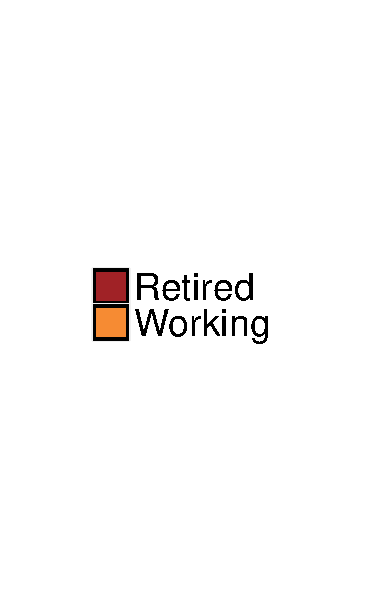
\includegraphics[width=3.5cm]{super-atlas/fig3-6-legend.pdf}}}
\begin{subfigure}{\columnwidth}
\captionsetup{skip=0pt, position=top, list=yes, justification=centering, labelsep=space, labelfont=bf, font={bf,small,theGrey}}
\caption{Singles}
\includegraphics[width=\columnwidth]{b5-super-atlas/Figure3-5orig-portrait.pdf}
\end{subfigure}
\vfil
\begin{subfigure}{\columnwidth}
\captionsetup{skip=0pt, position=top, list=yes, justification=centering, labelsep=space, labelfont=bf, font={bf,small,theGrey}}
\caption{Couples}
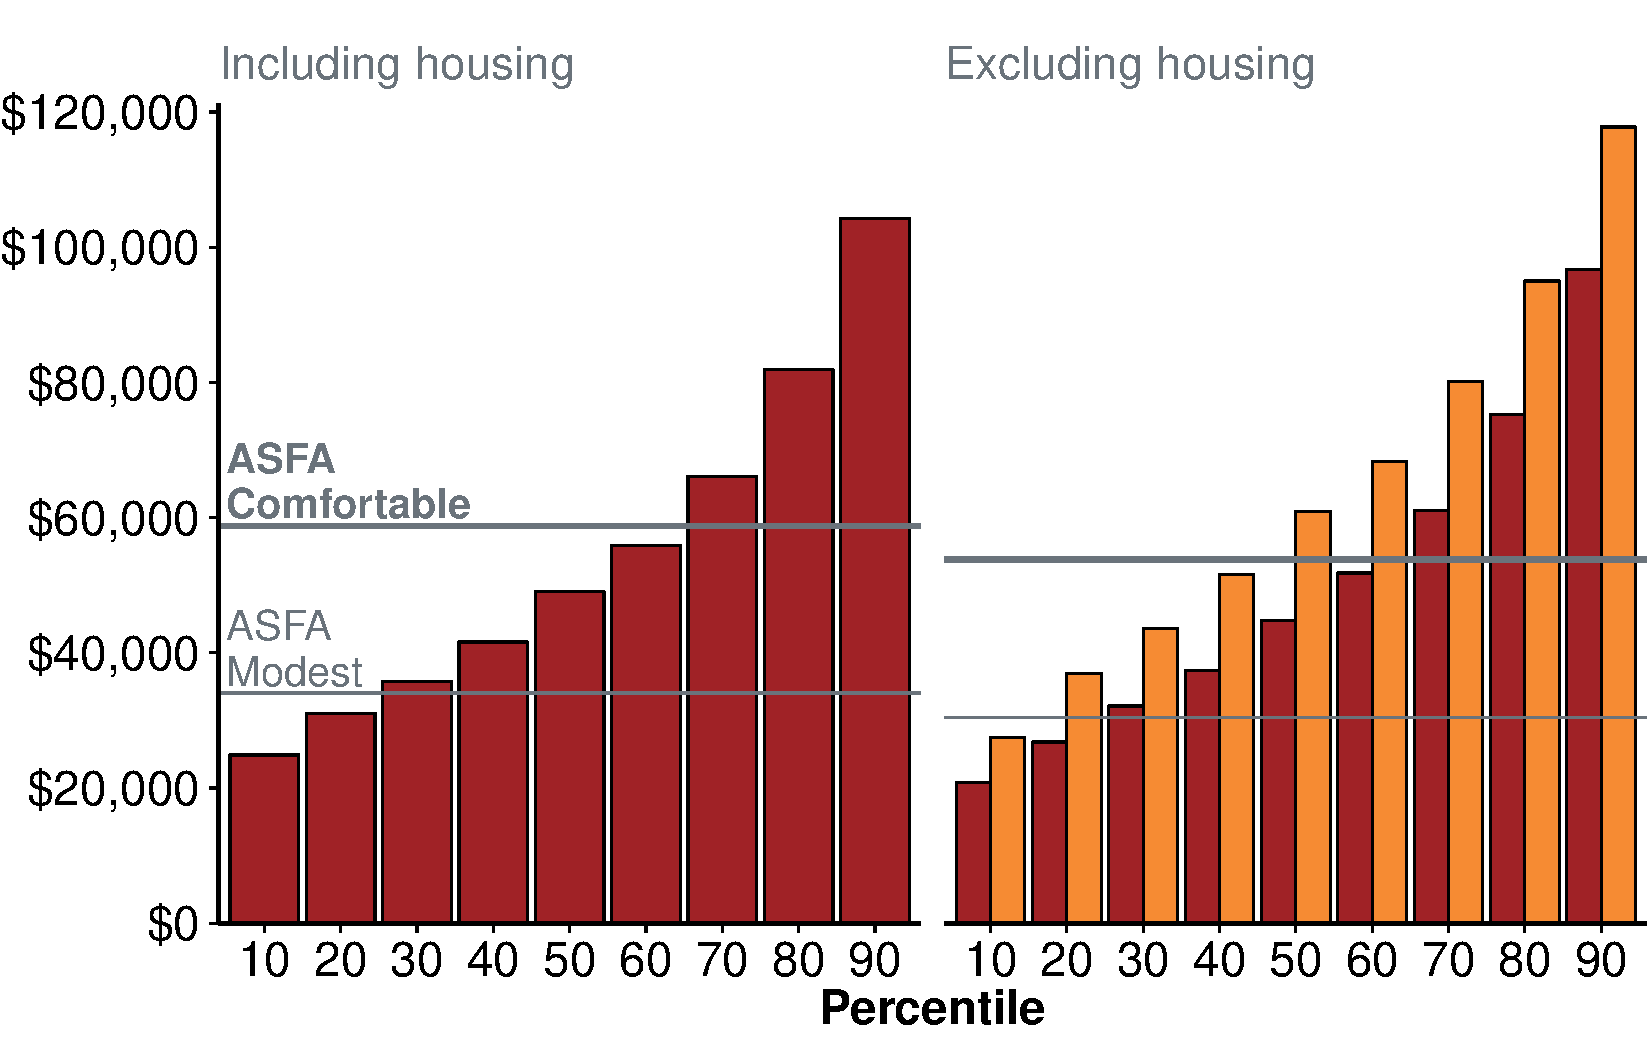
\includegraphics[width=\columnwidth]{b5-super-atlas/Figure3-6orig.pdf}
\end{subfigure}
\fnotes{fig:SUPER-3-5-3-6}{Expenditure of elderly single households (60-79) and working age (25-59) single household expenditure, by expenditure percentile. Expenditure variables have been inflated forward to 2015 levels using the change in final household consumption expenditure between June 2009 and March 2015. Left pane shows expenditure for elderly singles who own their own home outright, and who will probably have higher expenditure on average than households that do not own their own home outright. }

\source{\textcites{ABS2011HES0910}{ASFA2015}. Grattan analysis}
\end{figure*}
\setlength{\marginparsep}{\origmargparsep}}

A couple without assets that earned this much would only just qualify for a small part-rate Age Pension (\Vref{tbl:SUPER-3}). It may seem surprising that a household with a disposable income sufficient for an affluent lifestyle can qualify for a part Age Pension. This results from the ‘taper rate’ for the Age Pension, which is set so that those beyond pension age still have reasonable incentives to work part-time. Under the taper rate the pension is reduced by 50 cents for each additional dollar of income. The result is a small Age Pension for those with an income just over that sufficient for an affluent lifestyle. In practice, such households are also likely to be excluded from the Age Pension by the assets means test.


Thus, an individual consistently earning \$115,000 a year -- on the basis of their superannuation assets alone -- is unlikely to be eligible for a pension on retirement. However, some households that do not qualify for an Age Pension on retirement may nonetheless qualify later in life if they consume their savings in retirement – as the ASFA standards assume. Consequently, greater savings may be required to minimise future Age Pension liabilities.

In practice, however, most pensioners don’t draw down much of their assets. Australian Government data shows that less than 50~per cent of all pensioners draw down on their assets, and over 40 per cent of pensioners are net savers.\footnote{\textcite{Morrison2015TheBestFormOfWelfare}. Around 45 per cent of pensioners were net savers in the first five years of receiving the Age Pension, and 43 per cent drew down on their savings. In the final five years of receiving the pension, 43 per cent of pensioners were still net savers, while just a third drew down on their savings.}  
A recent study found that at death the median pensioner still had 90 per cent of their wealth as first observed.\footnote{\textcite{WuAsherMeyrickeEtAl2015} find that younger, wealthier pensioners tend to draw down on their savings but most pensioners are net savers later in life.} Another study found that many Australian retired households – pensioners or otherwise – do not spend down much of their financial wealth as they age.\footcite{SpicerStavrunovaThorp2015} This suggests that those who do not qualify for a pension on retirement are unlikely to draw down on their assets to the point that they start to qualify for a material Age Pension. 

In any case, the ASFA standard assumes that a household’s only income-earning asset in retirement is a superannuation fund built on compulsory contributions. In practice, someone earning \$115,000 annually is likely to save far more for their retirement than just their compulsory superannuation contributions (\Cref{sec:SUPER-3-2}), and as a result will have a retirement much more prosperous than the ‘affluent’ benchmark as defined by ASFA. 

Some commentators have suggested that retirees need an even higher super balance at retirement than that proposed by ASFA, and that Australians need savings of up to \$1 million in order to generate an adequate retirement income.\footcite{Cooper2015}  Their analyses typically assume that retirees are only prepared to invest their retirement savings in government bonds, currently yielding around 2.3 per cent. This is clearly unrealistic. Superannuation fund returns have averaged almost 6 per cent a year since 2000.\footnote{\gao\ \textcite{APRA2015JuneSuperPerformance}.} 
Such claims also ignore the role of the part Age Pension in boosting the retirement incomes of retirees with post-tax incomes of less than \$41,336 (singles) or \$66,446 (combined couples), and ignore any other financial savings outside of superannuation.%
% \enlargethispage*{-0.5\baselineskip} 

Other commentators have noted that sustained low investment returns may reduce the accumulated value of superannuation savings at retirement, leading to lower retirement incomes.  While lower returns are a risk to retirement incomes, it does not follow that more generous superannuation tax breaks should make up the difference. First, if investment returns are permanently lower, then the target living standard in retirement should also be lowered.\footcites[][9]{ActuariesInstitute2015RetirementIncomes}{Blayney2015} Second, increasing the generosity of superannuation tax breaks is an expensive way to boost the retirement incomes of low and middle-income earners, as this report makes clear. Most of the benefits from increasing superannuation tax breaks – such as from raising the annual cap on pre-tax contributions or lowering tax rates on super fund earnings – flow to high income earners that have larger savings. Instead, concerns about the adequacy of retirement savings in a world of lower investment returns should be addressed through changes to the Age Pension.

\section{Superannuation tax breaks are poorly targeted at those with variable incomes\label{sec:SUPER-3-4}}
What about those with more variable incomes? Concerns are sometimes raised about how annual limits on contributions can disadvantage people whose income varies a lot from year to year.\footcite[][5]{ASFA2015b} This is a common pattern for women who take time out of the workforce to have children. Overall, annual earnings tend to rise to about age 35, and then stay around that level until just before retirement.\footcite[][18,19,49--50]{DaleyWoodWeidmannEtAl2014}  

This argument assumes that there are a material number of people who return to the workforce after a substantial break and who have sufficiently high incomes that they can afford to make substantial contributions to superannuation. However, incomes in Australia tend to be persistent. The longitudinal dataset of the \textcite{HILDA2015} survey, which commenced in 2000, confirms that those who earn a lot in one year, tend to earn a lot for many years (\Vref{fig:SUPER-3-7}).


\begin{figure}
\captionsetup{margin={0cm,-0.25cm}, oneside, singlelinecheck=false}
\captionwithunits{Those who earn a lot in a year tend to earn a lot for many years}%
{Percentage of years in income decile for people of prime working age who are in top income decile at least once}\label{fig:SUPER-3-7}
% 
\includegraphics[width=\columnwidth,page=16]{super-atlas/PPTX.pdf}
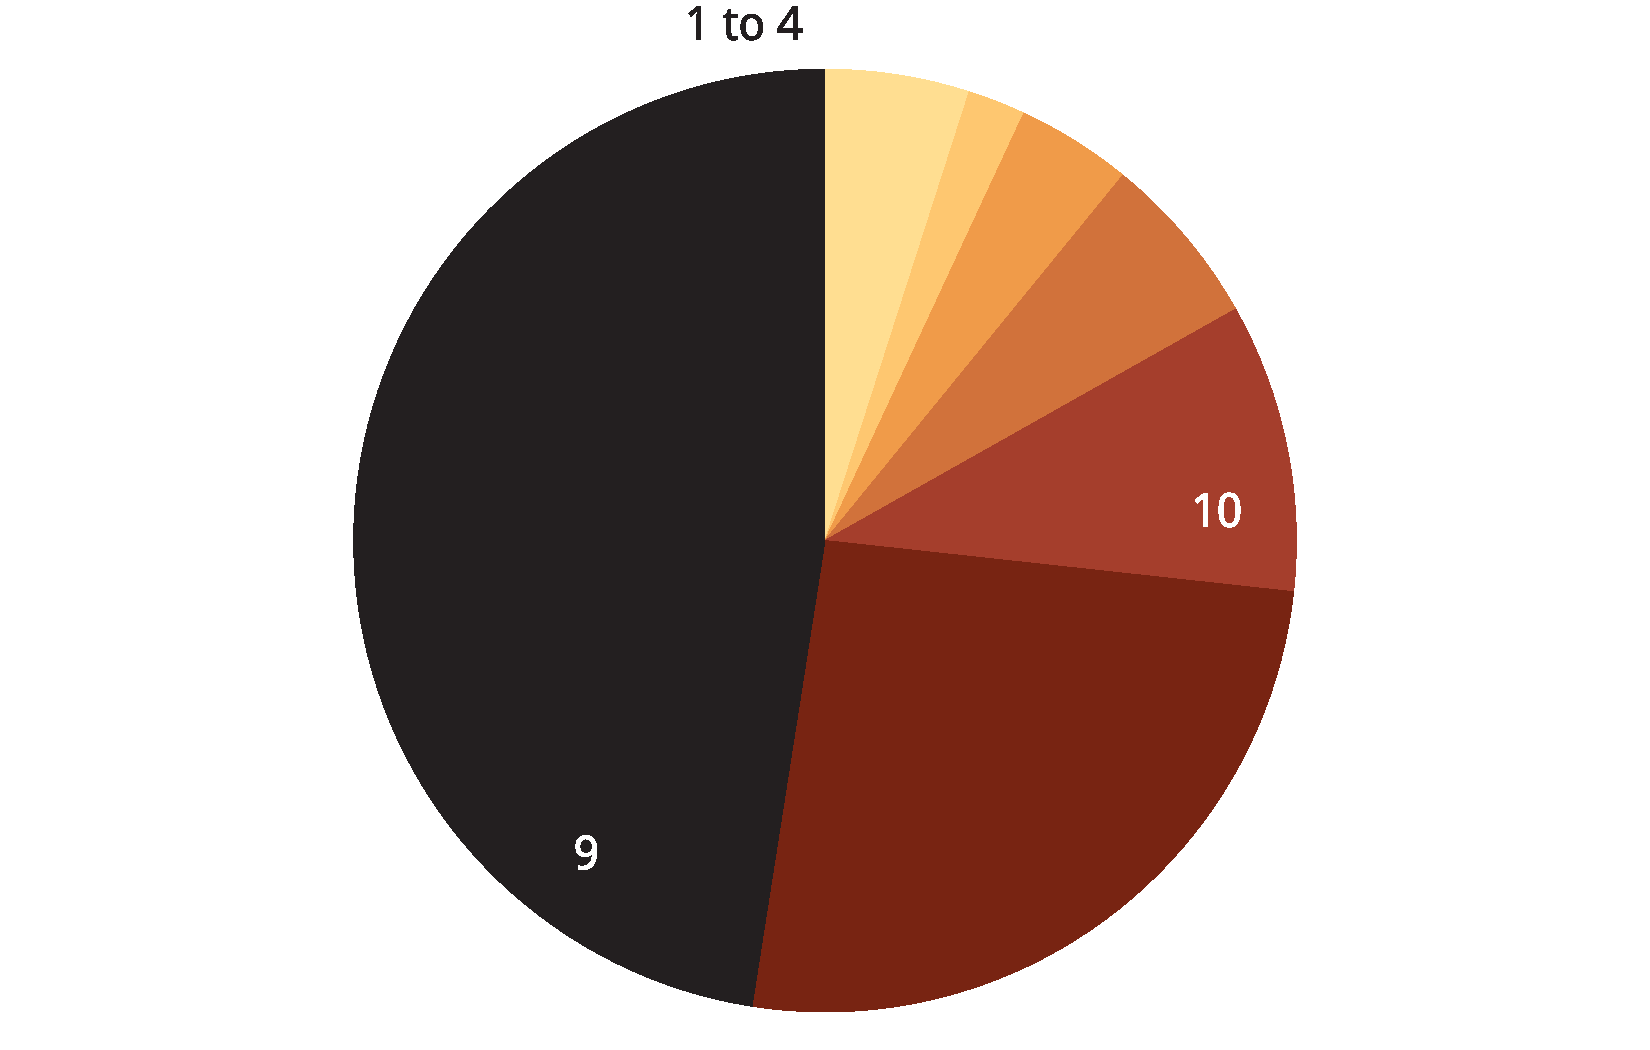
\includegraphics[width=\linewidth]{b5-super-atlas/Figure3-7-1.pdf}
\notes{Primary working age is defined as aged over 30 at the beginning of the survey and less than 60 at the end of the survey. Analysis of the 13 years of the HILDA survey. Income deciles are of population aged 15 and over.}

\source{\textcite{HILDA2015}}
\end{figure}

As the more detailed analysis in \Vref{fig:SUPER-3-8} shows, people of prime working age who are in the top income decile in any single year spent 85 per cent of the 13 years in which data was collected among the top 30 per cent of income earners. Overseas studies confirm the finding that most high-income earners in a given year tend to stay towards the top of the income distribution for most of their working lives.\footcite[][56]{LevellRoantreeShaw2015}  

\afterpage{%
\begin{figure}
\captionsetup{margin={0cm,-0.15\linewidth},oneside}
\captionwithunits{About a quarter of the population have just a single year earning a high income}%
{People of working age who were in the top decile at least once during the \textcite{HILDA2015} survey period}\label{fig:SUPER-3-8}
% \includegraphics[width=1.12\columnwidth,page=17]{super-atlas/newPPTX.pdf}
\makebox[\textwidth]{\includegraphics[width=1.182\linewidth]{figure_persistence_of_115k/marimekko-1.pdf}}
\notes{See notes for \Cref{fig:SUPER-3-7}.}

\source{\gao\ \textcite{HILDA2015}.}
\end{figure}
}

Although volatility over a 35 year period would be greater than over the 13 years of longitudinal data available in HILDA, clearly high incomes tend to persist.%
\footnote{For example, \textcite[][96]{ProductivityCommission2015-Tax-and-transfer-incidence}  finds that average income taxes for a given lifetime income align closely with the annual income taxes paid by someone with that same income in 2014-15, suggesting that people’s annual and lifetime incomes are closely related.}
Furthermore, high contributions to superannuation tend to be made later in life (\Vref{fig:SUPER-4-7} and \Vref{fig:SUPER-5-1}) when incomes tend to be more consistent.%
\footnote{\textcite{Karahan2015} also finds that a large shock to income becomes less likely as workers age, and then becomes more likely again after age 50.} 

Of course, some people, particularly women, do have variable incomes. But they are unlikely to be impacted much by limits that only affect those contributing more than \$11,000 a year. As shown in \Vref{fig:SUPER-4-6}, there are relatively few women who contribute more than \$10,000 a year. 

Policies to encourage adequate savings for those with irregular earnings need to be far more targeted. In practice, the current rules that allow substantial pre-tax and post-tax voluntary contributions to superannuation are overwhelmingly used by those with high incomes (\Vref{fig:SUPER-A-2} and \Vref{fig:SUPER-A-9}) and who already have high savings (\Vref{fig:SUPER-5-2}). 

The current tax breaks are an expensive way for government to boost retirement incomes for a relatively small group of lower income women making ‘catch up’ payments. If government wants to increase the retirement balances of women that have spent time out of the workforce, reinstating the Low Income Superannuation Contribution (LISC) would have far more impact on this group per government dollar than the current superannuation tax breaks. 

\section{Superannuation tax breaks for those on high incomes do not materially reduce Age Pension costs}\label{sec:SUPER-3-5}
As high-income earners are likely to save and self-fund their own retirement anyway, superannuation tax concessions that benefit this group do little to reduce future Age Pension liabilities. Treasury projections show that the lifetime value of tax breaks to high-income men is much higher than the value of the Age Pension for low-income earners (\Vref{fig:SUPER-3-9}). 

\begin{figure}
\captionwithunits{Superannuation tax breaks for high-income earners cost more than Age Pension payments to others}%
{Net present value of the projected lifetime cost of government support for retirement incomes (2010 dollars)}\label{fig:SUPER-3-9}
% 
\includegraphics[width=\columnwidth,page=18]{super-atlas/PPTX.pdf}
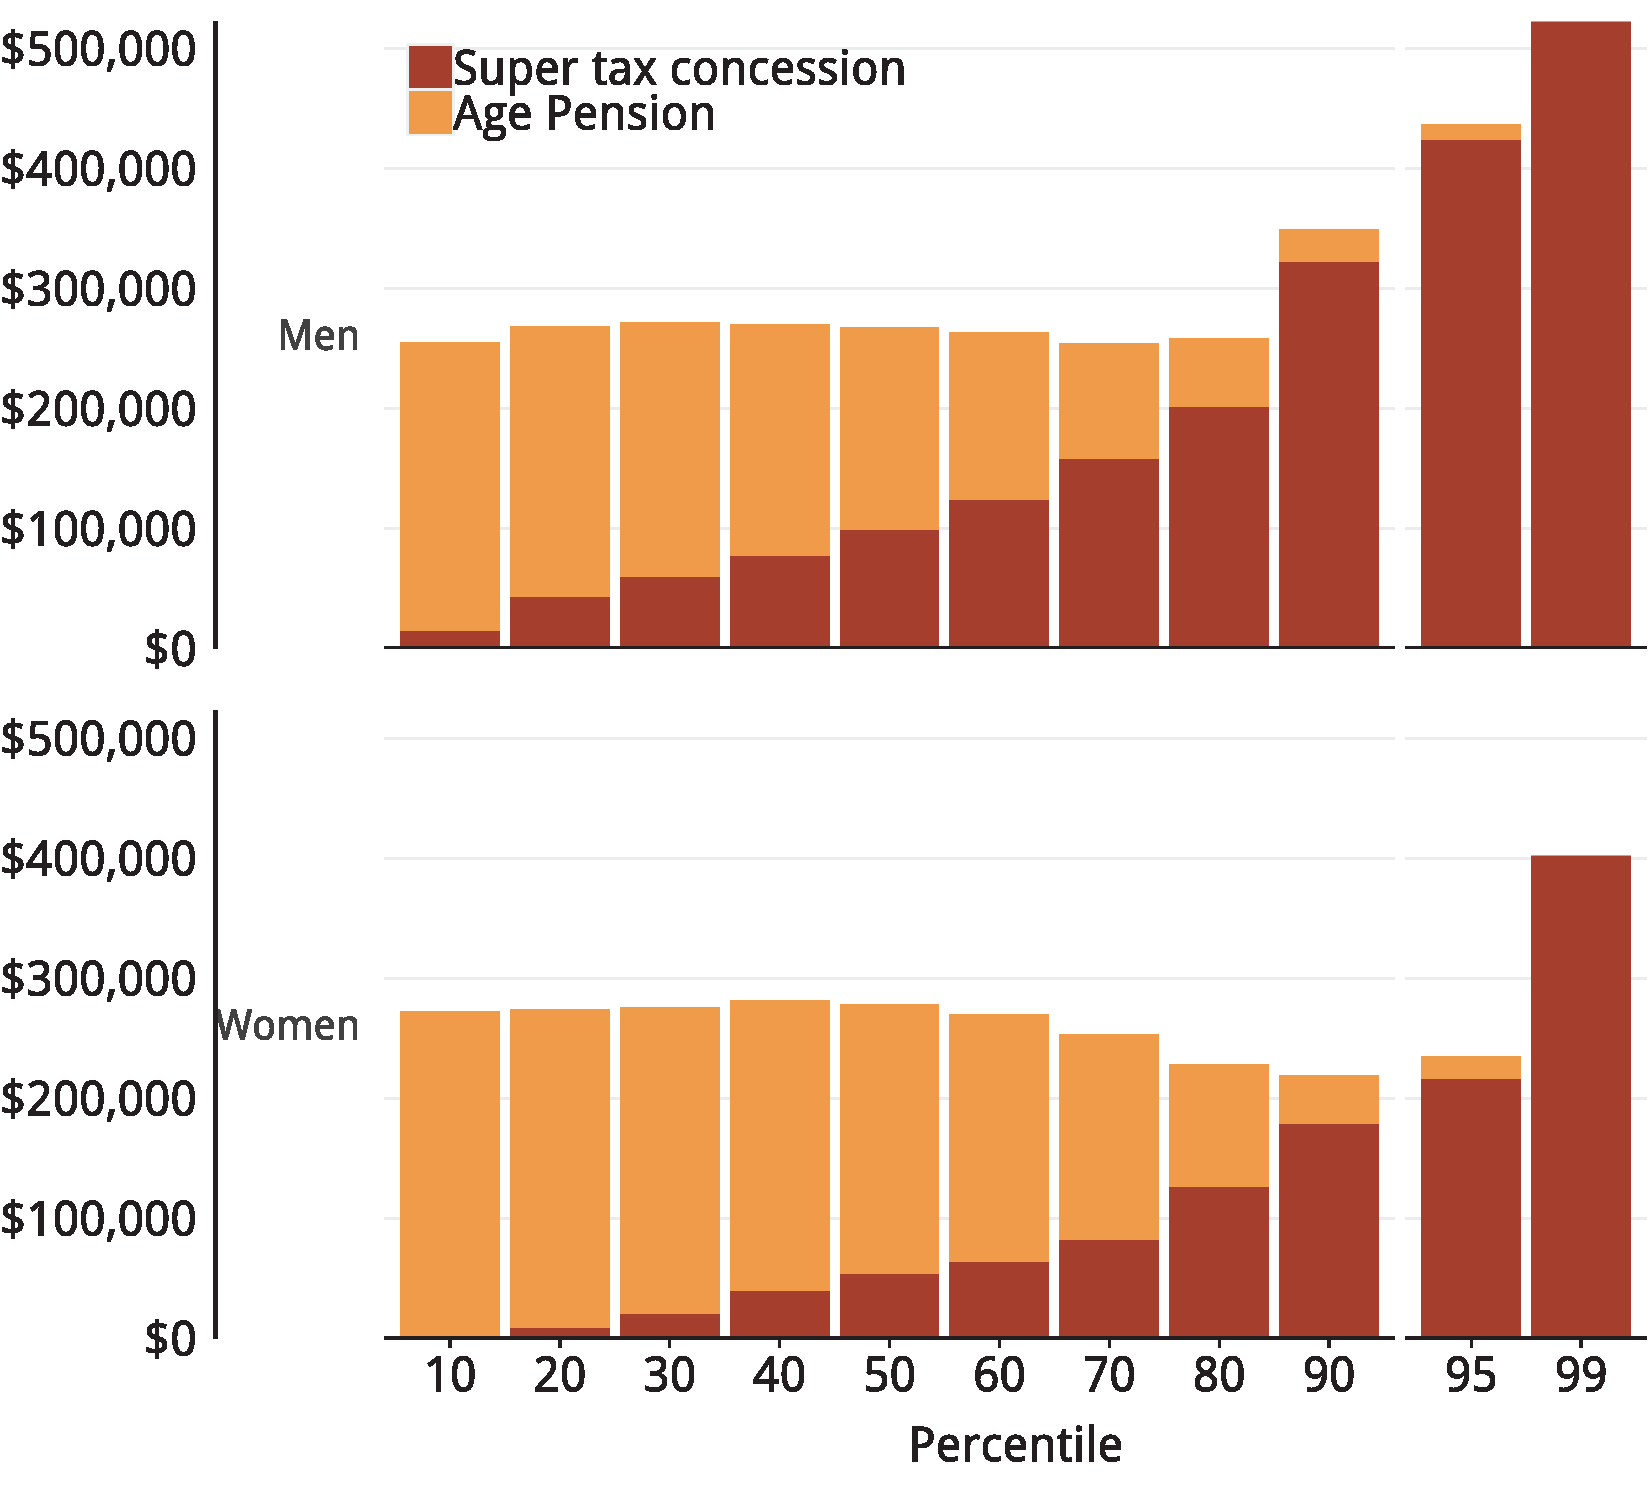
\includegraphics[width=\linewidth]{b5-super-atlas/Figure3-9-1.pdf}
\fnotes{fig:SUPER-3-9}{Net present value of lifetime cost to government includes Age Pension payments and net tax expenditures of those aged 30 in 2010; assumes life expectancies of 88 years for males, 90 years for females; pre-tax investment returns of 6.5 per cent, annual wages growth 4.14 per cent; all income groups except the 99th percentile are assumed to fully draw down their superannuation balances by death; excludes Division 293 tax. \\[4pt]
This calculation may substantially understate the lifetime cost of super tax breaks for those in the top 20 per cent of income earners. They tend to make large post-tax contributions close to retirement (\Vrefrange{fig:SUPER-5-1}{fig:SUPER-5-2}). Consequently, in retirement their total super balances, and the value of the earnings tax breaks, are much higher than would be expected from analysing the distribution of pre-tax contributions (\Vref{fig:SUPER-6-1}), which appear to underlie Treasury's estimates for the lifetime cost of tax breaks.%
}

\source{\textcite{Treasury2012ReviewMacroRevenueForecasts}}
\end{figure}

ASFA has criticised this analysis because it assumes that people remain in the same income percentile amongst their age group for their entire working life.\footcite[][7--8]{Clare2012}  As shown by \Cref{fig:SUPER-3-8}, incomes are persistent, but not as persistent as this. 

However, the Treasury projections make other assumptions that substantially understate the tax breaks for high-income earners. They do not account for post-tax contributions, which are concentrated amongst high-income earners and provide large breaks on super earnings in retirement.\footnote{For example, \textcite{Blayney2015} estimates that 75 per cent of the accumulated lifetime value of investment returns occurs beyond the age of 60 years.}  Different assumptions about life expectancy and draw-down rates can also result in much higher estimates of the lifetime benefits for high-income earners.  Industry Super calculates that superannuation tax breaks for the top 5 per cent of income earners are worth more than \$2~million for men over their lifetimes.%
\footnote{For single men retiring to 2055. The projected lifetime cost of super tax breaks for single women in the top 5~per~cent of income earners is \$1.6~million.} 

Thus the substantial superannuation tax breaks for high-income earners do little to serve the purposes of superannuation: to encourage savings to replace and supplement the Age Pension. High-income households are very likely to self-fund their retirement, irrespective of superannuation tax breaks, and consequently they are unlikely to qualify for an Age Pension. 

The primary effect of superannuation tax breaks on this group is to make them even richer in retirement, without either affecting their savings behaviour, or reducing government pension liabilities.

\section{Superannuation tax breaks cannot be justified as compensation for not receiving the Age Pension}\label{sec:SUPER-3-6}
Some have suggested that superannuation tax concessions to high-income earners are nevertheless fair because they provide government support equivalent to that provided through the Age Pension to the less well off (see \Vref{fig:SUPER-3-9}).\footcite[][46]{ASFA2015TreasurySubmission}  

However, this muddles a tax break with a welfare payment. To use an analogy, wage earners don’t expect tax breaks equivalent to Newstart payments. That is because, by definition, welfare payments are made to those who otherwise lack resources. The purpose of the Age Pension is to provide all Australians with a safety net in retirement so that they have enough money for a reasonable minimum standard of living when many are no longer able to work. As with other welfare payments, the Age Pension is targeted – via the income and assets means tests – to those in need. 

\section{\mbox{Superannuation tax breaks need to be targeted to meet their policy aims}}\label{sec:SUPER-3-7}
The targeting of superannuation tax breaks will never be perfect. Superannuation will be far too generous for most households if the limits are set so that a sole breadwinner can save enough assets solely in super to support a couple in retirement without recourse to an Age Pension. In practice, each member of couple households will have their own superannuation, and will typically have other assets outside of superannuation and their home.

If we consider the way tax breaks currently operate in Australia’s superannuation system overall, it is clear that they are very poorly targeted at promoting additional retirement savings that reduce Age Pension liabilities.

% Tough to typeset
\newcommand{\outerbf}[1]{\textbf{#1}}
\newcommand{\emphbf}[1]{\textit{#1}}
\begin{enumerate}
\item \outerbf{\emphbf{Compulsory} contributions from \emphbf{pre-tax} income} do increase retirement savings for middle-income earners (\Cref{sec:SUPER-2-6}), and the associated tax concessions are arguably reasonable compensation for the compulsion to lock up earnings in superannuation (\Cref{sec:SUPER-2-4}). But they still most benefit those on higher incomes who make larger compulsory contributions (\Cref{fig:SUPER-A-1}).
\item \outerbf{\emphbf{Voluntary} contributions from \emphbf{pre-tax} income} are mostly made by those aged over 50 – and therefore relatively close to the age of 60 at which they can start to withdraw these contributions. Those in the top fifth of income earners make over half of all voluntary pre-tax contributions (\Cref{fig:SUPER-4-4}). 
\item \outerbf{\emphbf{Voluntary} contributions from \emphbf{post-tax} income} are dominated by those already over 60. These contributions rarely increase retirement savings – they are primarily funded from funds already saved by those entitled to retire (\Cref{fig:SUPER-5-1}). 
\end{enumerate}


Better targeting superannuation tax breaks does not imply removing all contributions tax breaks for those earning more than \$115,000 a year. However, the proposals set out later in this report would reduce them so that in absolute terms the tax breaks for high-income earners are not much bigger than the tax breaks for those earning less. 

\section{Previous reforms to superannuation tax breaks were piecemeal}\label{sec:SUPER-3-8}
Governments have repeatedly tweaked the tax breaks on superannuation contributions, but none of these changes have made much difference compared to the total size of the tax breaks. Given the escalating cost of superannuation tax breaks, more substantial reforms are needed to ensure budget sustainability. 

Governments have changed the amounts that can be contributed to superannuation from pre-tax earnings many times, as shown in \Cref{tbl:SUPER-3}. Collectively these changes over the last eight years have improved the budget bottom line by around \$1~billion per year.\footnote{\gao\ \textcite{TreasurymultipleyearsBudgetPapers200809to201516}.}  

The value of superannuation contribution concessions for high-income earners were also reduced in 2012 when the Labor Government increased the tax rates on concessional superannuation contributions for individuals with income greater than \$300,000, from 15~per cent to 30~per cent. Treasury estimated that this reform, known as \defi{Division~293} tax, would boost revenue by \$475~million in~2015-16.\footcite[][41]{Treasury2012} 

\begin{table}
\caption{Annual caps on pre-tax contributions to superannuation}\label{tbl:SUPER-4}
\begin{tabularx}{\columnwidth}{lRRRR}
\toprule
& \multicolumn{2}{c}{General cap} & \multicolumn{2}{c}{Age-based higher cap} \\
\cmidrule(lr){2-3}\cmidrule(lr){4-5}
Year    & Age                & Cap &  Age &  Cap \\
\midrule
2007-08 & under 50 & \BfUpArr\ \$50,000 & over 50 &\BfDnArr\ \$100,000 \\
2009-10 & under 50 & \BfUpArr\ \$25,000 & over 50 & \BfDnArr\ \phantom{1}\$50,000 \\
2012-13 & (all)    &          \$25,000 &\BfDnArr\ \phantom{ove.}\textcolor{theGrey}{n/a}  \\
2013-14 & under 59 &          \$25,000 & over 59                      & \BfUpArr\ \phantom{1}\$35,000 \\
2014-15 & under 49 & \BfUpArr\ \$30,000 & \BfUpArr\  over 49 & \$35,000 \\
\bottomrule 
\end{tabularx}
{\footnotesize
\begin{tabularx}{\linewidth}{Rr}
%
\BfUpArr & \footnotesize{tax concession more generous} \\ 
\BfDnArr & \footnotesize{tax concession less generous}
\end{tabularx}%
}%
\vspace*{5pt}
\tnotes{tbl:SUPER-4}{%
Under 35s could only contribute \$15,260, while those aged 35 to 49 could contribute \$42,385, and those aged 50 and over could contribute up to \$105,113. The former Labor government sought to increase the pre-tax contributions cap for over 50s to \$50,000 in the 2010-11 Budget for those with superannuation balances below \$500,000, but this measure was dropped following industry consultation.}

\source{\textcites{ATO2015h}{SimplifiedSuperAct2007}{SwanShorten2013}}\DEVIATION{}
\vspace{5pt}
\end{table}


The incoming Abbott Government announced the abolition of the LISC\phantomsection
\label{sec:SUPER-LISC-to-be-abolished} from 2017-18, at a saving of around \$1 billion in 2017-18.\footcite[][94]{Treasury2013MYEFO1314}  The LISC refunds contributions tax for low-income earners, who would pay little or no income tax on the income they are forced to contribute to super. Once the LISC is abolished, those earning less than \$18,001 will pay higher tax on their superannuation contributions than on their take-home pay.\footcite{ATO2015LISC} 

Other government programs to support the superannuation balances of low-income earners have also been reduced in the search for budget savings. The former Labor government temporarily reduced the matching rate for government co-contribution available to low-income taxpayers who made a post-tax superannuation contribution from 150 per cent to 100 per cent in the 2009-10 Budget.\footnote{\textcite{Treasury2009BudgetPapers0910}. The super co-contribution was first introduced by the former Coalition government in 2003. The government originally provided a matching co-contribution\DEVIATION{} of 150 per cent on the first \$1,000 of post-tax contributions made by low-income taxpayers.}   
This reduction was made permanent in the 2010-11 Budget.\footcite[][298]{Treasury2010Budget1011no2}  
The matching rate for the government co-contribution was reduced again to 50 per cent in the Government’s 2011-12 mid year fiscal update.\footcite[][291]{Treasury2011MYEFO1112} 

Thus superannuation tax breaks need more substantial reform. They are an unfair and costly way to promote retirement savings. Most of the value goes to people on higher incomes who are likely to save anyway, unlikely to qualify for an Age Pension, and not in need of government support. And by definition, other taxpayers (often younger and less well off) pay more in tax to make up for superannuation tax breaks. The frequent but minor changes over the last decade have left a large gap between the purposes of superannuation and its outcomes. Further changes to the rules, which undermine stability and confidence in the system, will continue until super tax breaks are targeted at the purpose of the system.


\section{Superannuation tax breaks should be reformed in a principled way\label{sec:SUPER-3-9}}
The remainder of this report investigates how the superannuation tax breaks should be reformed so that they are more tightly targeted at their purposes. 

A number of principles should apply to any reforms to superannuation tax breaks:
\begin{enumerate}
\item Tax breaks that \textbf{don't serve the policy purpose} of replacing of supplementing the Age Pension should be minimised.
\item	Tax breaks that \textbf{do encourage savings to replace or supplement the Age Pension} should be preserved. 
\item	Where possible, \textbf{equity} should be maximised. This implies that superannuation should aim to provide more benefits to those on low incomes than those on high incomes. But this is not the primary focus of the superannuation system. Progressivity should primarily be achieved through the welfare and income tax system. On the other hand, superannuation tax breaks should not be designed for the primary purpose of reducing the progressivity of the income tax system. 
\item	The \textbf{budgetary costs} of superannuation tax breaks should be minimised unless they are justified by the social benefits of those tax breaks.
\item	The system must be \textbf{administratively workable}. This needs to take into account both the starting point of systems in place, as well as the transitional issues of reform.
\end{enumerate}

Of course these principles do not always work in lockstep. Some arrangements may marginally increase savings that serve the purposes of superannuation, but result in very large tax breaks for people who were going to save for their own retirement anyway. In assessing any reform, it is important to look at the balance of likely impacts.



\chapter{Contributions tax breaks}
While about two thirds of contributions to superannuation are compulsory, the remaining third are ‘voluntary’ contributions. All compulsory contributions are ‘concessional’ – that is, they are made from pre-tax income. Of the voluntary contributions, about a quarter are pre-tax; the remainder are made from post-tax income.

The tax breaks on contributions disproportionately benefit high-income earners: they save more tax per dollar contributed, and they contribute more dollars. Voluntary pre-tax contributions over \$10,000 in a year are mostly about tax planning rather than adding to net savings. Those contributing more than \$10,000 a year are predominantly high-income men aged over 50. 

As a result, the tax breaks for contributions of more than \$10,000 a year primarily benefit those who would have self-funded their retirement anyway. Indeed, around 24 per cent of voluntary pre-tax contributions are made by those aged over 60, entitled to withdraw their contributions immediately.\footnote{\gao\ \textcite{ATO2015SampleFile1213}.\DEVIATION{}} 

The best way to reform these tax breaks would be to limit concessional contributions to a maximum of \$11,000 per year. This change would target superannuation tax breaks to those who need them to reduce and replace their Age Pension. It would be relatively easy to implement, and would improve the budget bottom line by around \$3.9 billion a year.

\section{\mbox{Superannuation contributions are made and taxed in a variety of ways}}
Australians contributed around \$115~billion to superannuation in 2012\nobreakdash-13 (\Vref{fig:SUPER-4-1}). %\enlargethispage*{0.25\baselineskip}


\begin{figure}
\captionwithunits{About 40 per cent of superannuation contributions are voluntary, mostly from post-tax income}%
{Total contributions to all superannuation funds, \$\ billions}\label{fig:SUPER-4-1}
% 
\includegraphics[width=\columnwidth,page=19]{super-atlas/PPTX.pdf}
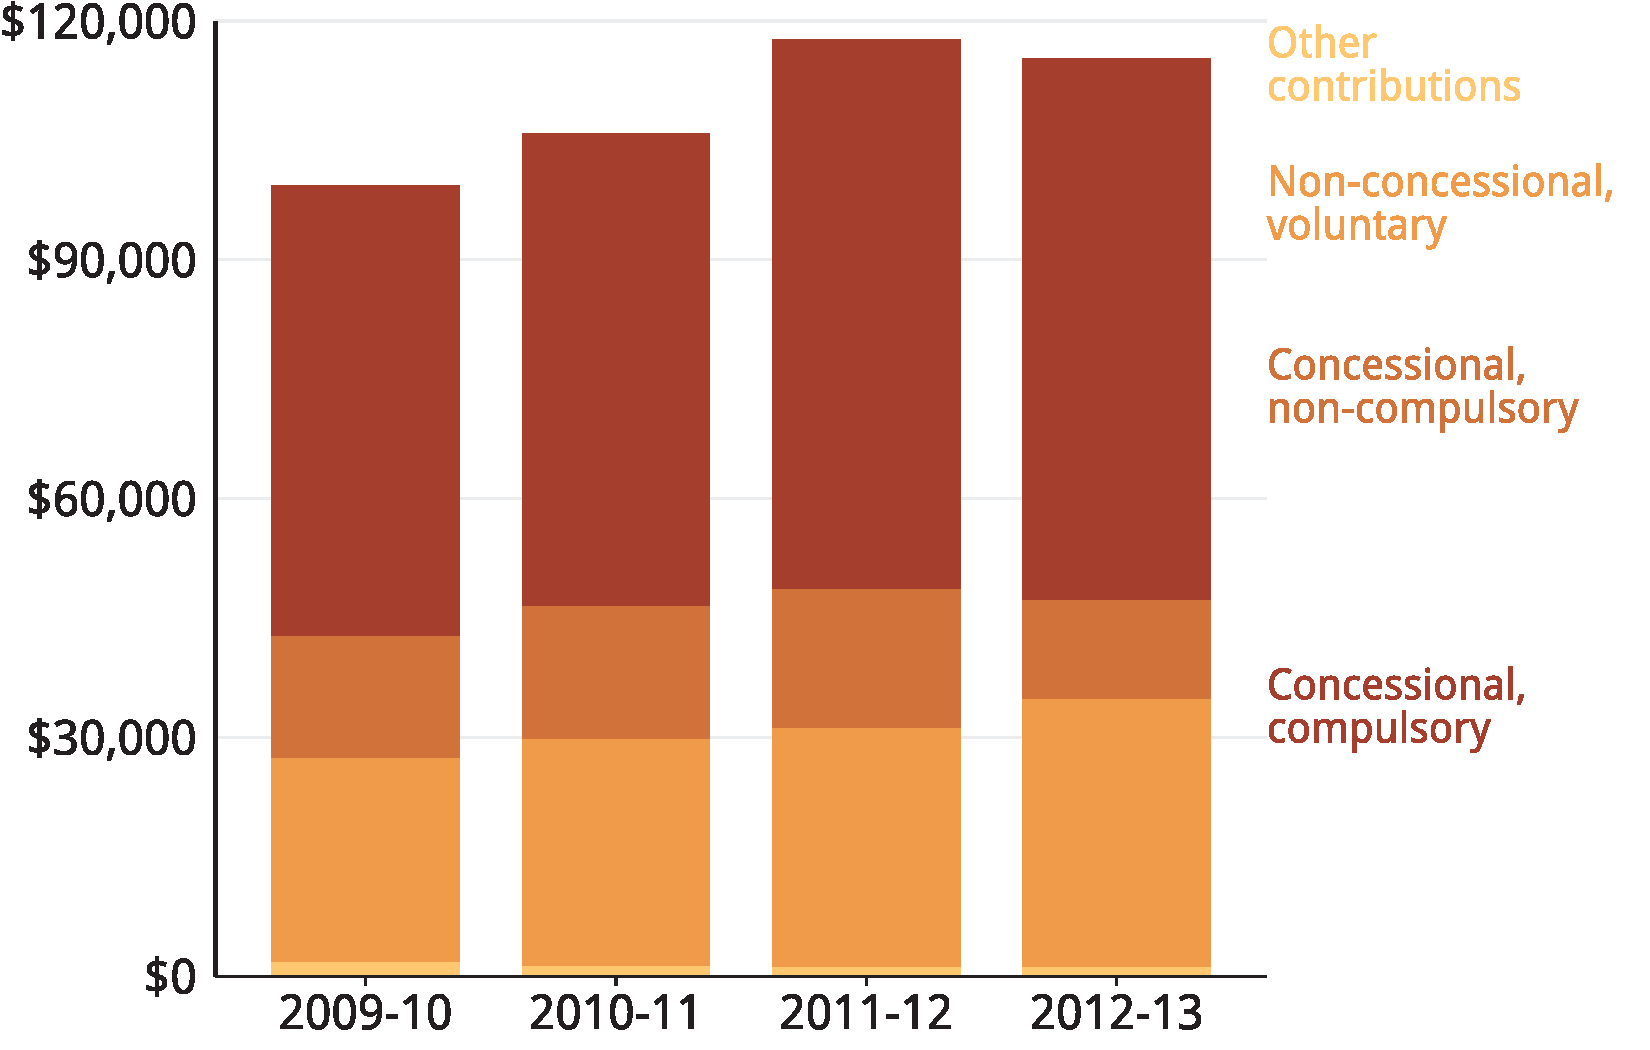
\includegraphics[width=\linewidth]{b5-super-atlas/Figure4-1-1.pdf}
\fnotes{fig:SUPER-4-1}{Compulsory pre-tax contributions are total employer contributions reported by APRA, including defined benefit contributions, less reportable employer (\ie~salary sacrificed) contributions reported by the ATO; voluntary pre-tax contributions are the sum of reportable employer contributions and reportable personal contributions reported by the ATO; voluntary post-tax contributions are total member contributions reported by APRA, less reportable personal contributions reported by the ATO; other contributions include spouse contributions and government co-contributions, and are drawn from APRA figures.}
\source{\textcites{APRA2014}{ATO2015Taxstats1213}. Grattan analysis.}
\vspace{\baselineskip}
\end{figure}

\textbf{Pre-tax contributions} make up 70 per cent of the total. A flat rate of 15 per cent tax is usually paid on these contributions once they enter the super fund, which is normally much less than the contributor’s marginal income tax rate. If the contributor earns more than \$300,000, a flat rate of 30 per cent tax is paid on these contributions.

Most pre-tax contributions – 60 per cent of all contributions – are \textbf{compulsory contributions}, which employers are required to make, at the super guarantee rate of 9.5 per cent on the first \$200,000 of an employee’s earnings.%
\footnote{\textcites{APRA2014}{ATO2015SampleFile1213}{ATO2015MaxSuperContrBase}. `Compulsory' contributions also includes employer contributions beyond the 9.5 per cent super guarantee rate that are negotiated as part of collective agreements. These additional contributions beyond the SG rate are estimated to account for around 7 per cent of ‘compulsory’ contributions, and cover almost 1 million workers \textcite[][16]{Kelly2013}.}  

\textbf{Voluntary pre-tax contributions} – 10 per cent of all contributions – are made when a worker salary sacrifices some of their earnings into superannuation, or claims a tax deduction on superannuation contributions (if self-employed).%  
\footnote{Income earners that do not have an employer making super contributions on their behalf, such as the self-employed, can access contributions tax concessions by claiming a tax deduction on super contributions they make directly to their super fund out of post-tax income.}
Pre-tax contributions are now capped – at a total of \$30,000 for compulsory and voluntary pre-tax contributions combined if the contributor is aged under 50, and \$35,000 if the contributor is over~50.

Annual contribution flows into superannuation funds can be volatile. The recent decline in superannuation contributions in 2012-13, particularly for voluntary concessional contributions, likely reflects the reduction in the cap on pre-tax contributions for those aged 50 years and over from \$50,000 to \$25,000, as well as the introduction of higher taxes on concessional contributions for high-income earners (Division~293 tax). The recent plateau in compulsory pre-tax contributions may also reflect weak wages growth, and a decline in the proportion of employees receiving employer contributions beyond the SG contribution rate.\footcite[][15--16]{Kelly2013}

\section{Generous tax breaks for pre-tax contributions disproportionately benefit high-income earners}
People who earn more get the biggest benefits from superannuation contribution tax breaks, both as a percentage of their income and in absolute amount. 

Those earning between \$180,000 and \$300,000 per year save 30~cents of tax for each dollar contributed (\Vref{fig:SUPER-4-2}).  The majority of taxpayers – earning less than \$80,000 a year – save 17.5~cents or less for each dollar contributed. By contrast, those earning between \$18,200 and \$37,000 only save 4~cents of tax for each dollar contributed.  For those earning less than \$18,200 per year, the 15~per~cent tax on superannuation contributions increases their tax, since their income is otherwise tax-free. The Low Income Super Contribution currently refunds this tax paid by low-income earners, but is due to be abolished from 2017-18 onwards (See \Cref{sec:SUPER-LISC-to-be-abolished} at page~\pageref{sec:SUPER-LISC-to-be-abolished}).

\begin{figure}[hp]
\captionwithunits{Contributions tax concessions provide the biggest discount to those on high incomes}{Tax rate}\label{fig:SUPER-4-2}
% 
\includegraphics[width=\columnwidth,page=20]{super-atlas/PPTX.pdf}
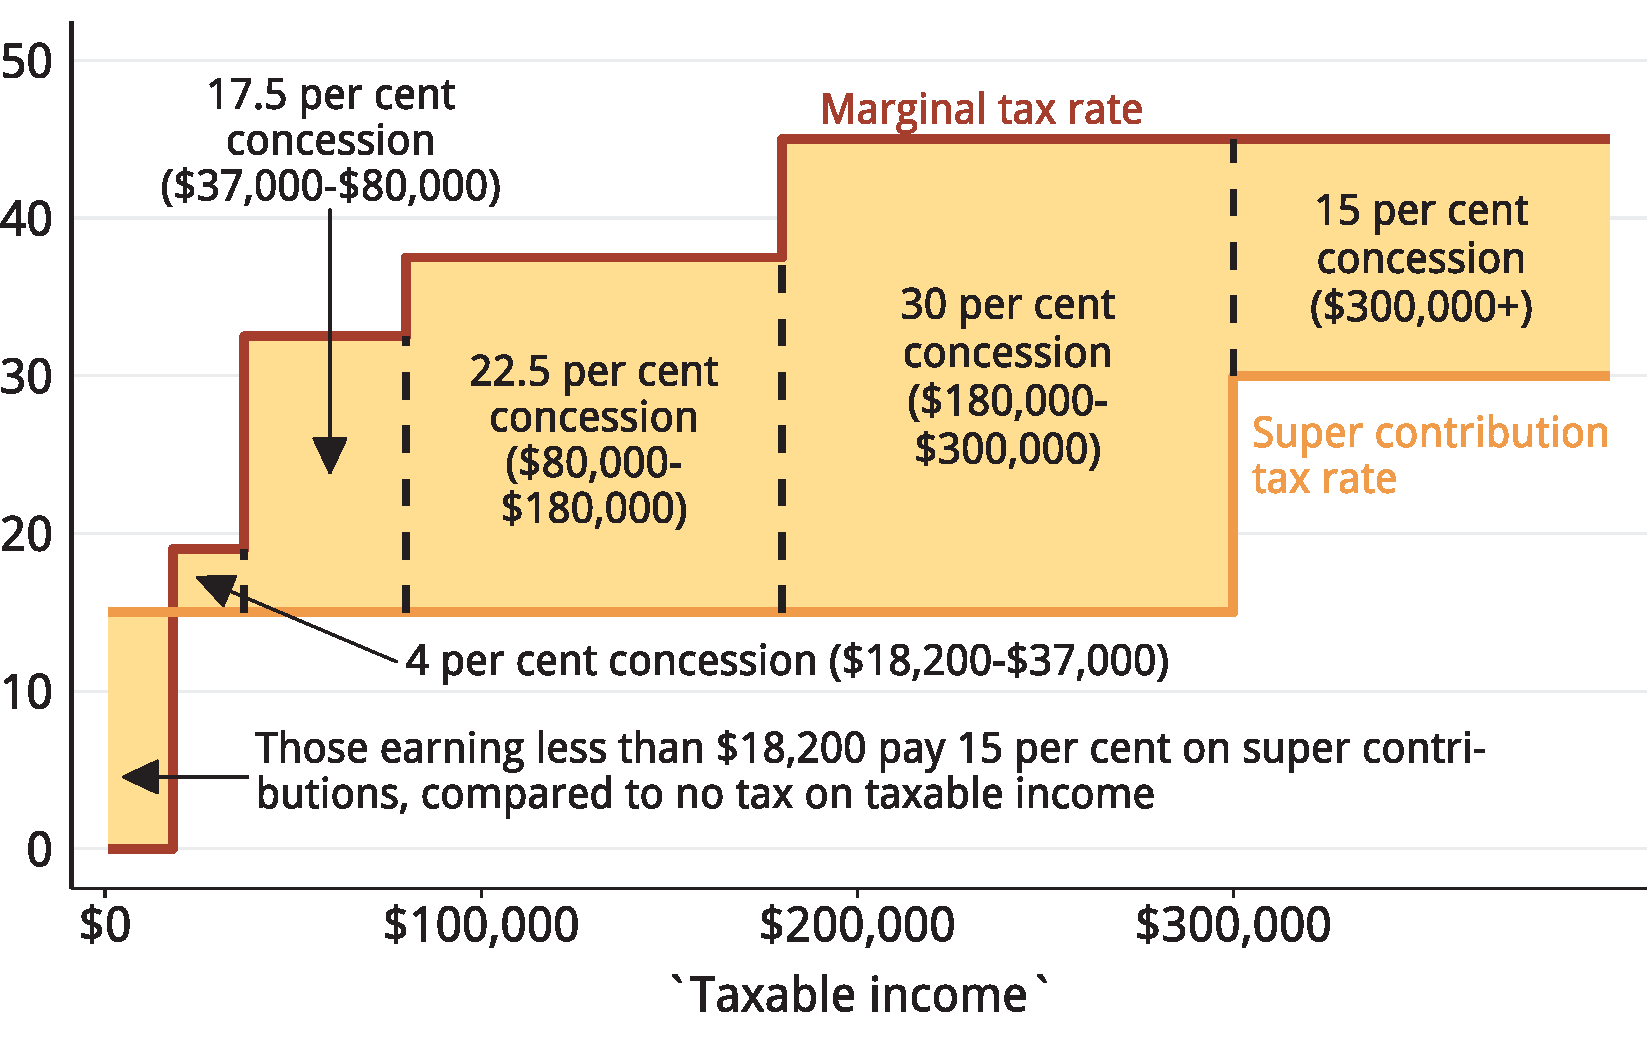
\includegraphics[width=\linewidth]{b5-super-atlas/Figure4-2-1.pdf}
\fnotes{fig:SUPER-4-2}{Does not include the Medicare Levy, Low Income Tax Offset or\DEVIATION{} the Temporary Budget Repair Levy. Division 293 tax applies to all contributions where the sum of taxable income and pre-tax super contributions exceeds \$300,000.}

\source{\textcite{ATO2015r}; Grattan analysis.}
\end{figure}

High-income earners not only save more tax per dollar contributed, they contribute many more dollars to superannuation. (\Vref{fig:SUPER-4-3}, and see also \Cref{fig:SUPER-A-1}). Their compulsory contributions are larger (because their wages are higher), and they make higher voluntary contributions (presumably because with higher incomes it is easier for them to save more). 

\begin{figure}
\captionwithunits{Those on high incomes make larger voluntary contributions, increasing the value of contributions tax breaks}%
{Average superannuation contributions for 2012-13 (in 2012-13 dollars)}\label{fig:SUPER-4-3}
% 
\includegraphics[width=\columnwidth,page=21]{super-atlas/PPTX.pdf}
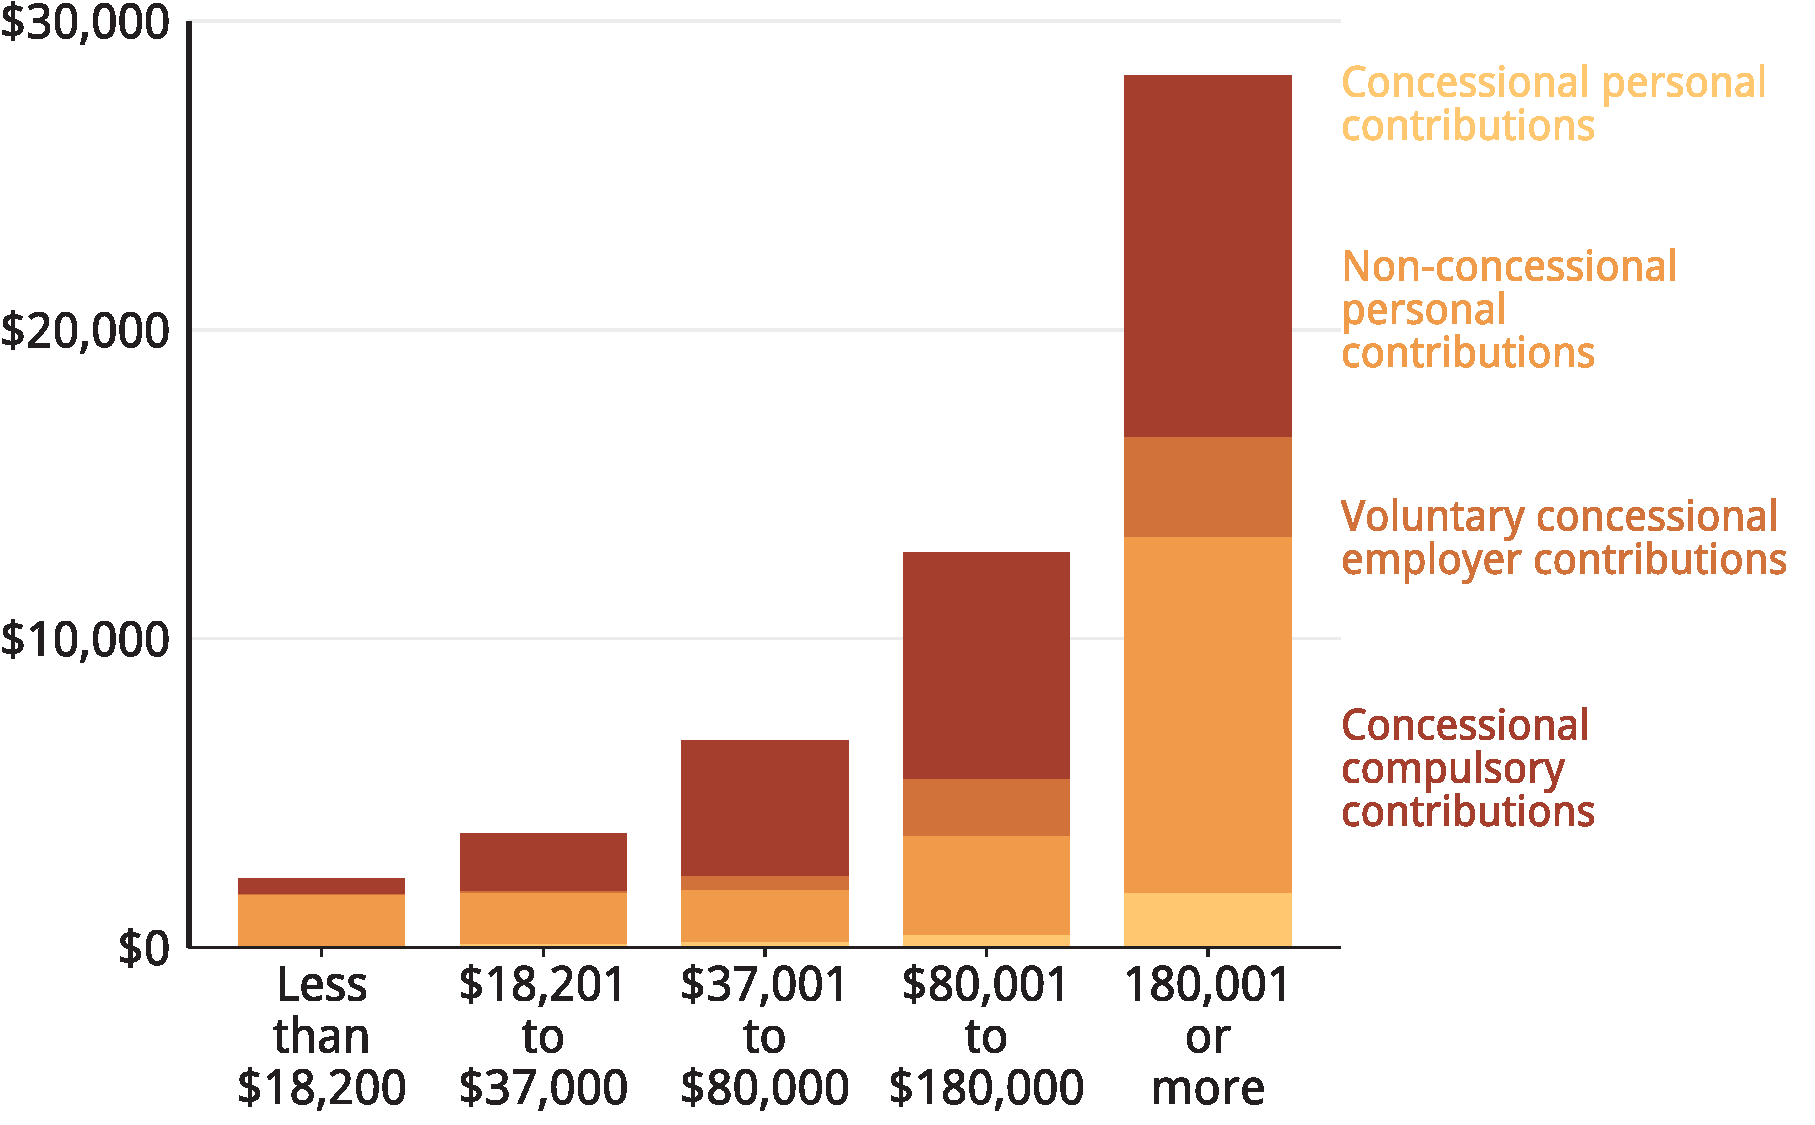
\includegraphics[width=1.1\linewidth]{b5-super-atlas/Figure4-3-1.pdf}
\fnotes{fig:SUPER-4-3}{The statistics for the 2012-13 income year were sourced from 2013 individual income tax returns processed by 31 October 2014 and member contributions statements received before 8 July 2015; Post-tax personal contributions are sourced from member contribution statements. Generally this represents contributions made to super from after personal tax income; Pre-tax personal contributions are sourced from individual income tax returns.}

\source{\textcites{ATO2015-Ad-hoc-Super-contr-by-age-income-balance-201213}{ATO2015SampleFile1213}; Grattan analysis.}
\end{figure}

In the over-50s age bracket pre-tax contributions from the top 10 per cent of income earners exceed those of the bottom 60 per cent combined (\Vref{fig:SUPER-4-4}, and see also \Vref{fig:SUPER-A-3}). Indeed, this understates the skew: many low-income earners do not file a tax return and therefore would not be included in the ATO data analysed. 

\Cref{fig:SUPER-4-4} also highlights the generosity of the current cap on pre-tax contributions. Even the top 10 per cent of income earners over the age of 50 usually contribute only around half of the \$30,000/\$35,000 pre-tax contributions cap. 

\begin{figure}[!tp]
\captionwithunits{Contributions among over 50s are heavily skewed towards high-income earners}%
{Average concessional contributions in 2012-13 for people over 50}\label{fig:SUPER-4-4}
% 
\includegraphics[width=\columnwidth,page=22]{super-atlas/PPTX.pdf}
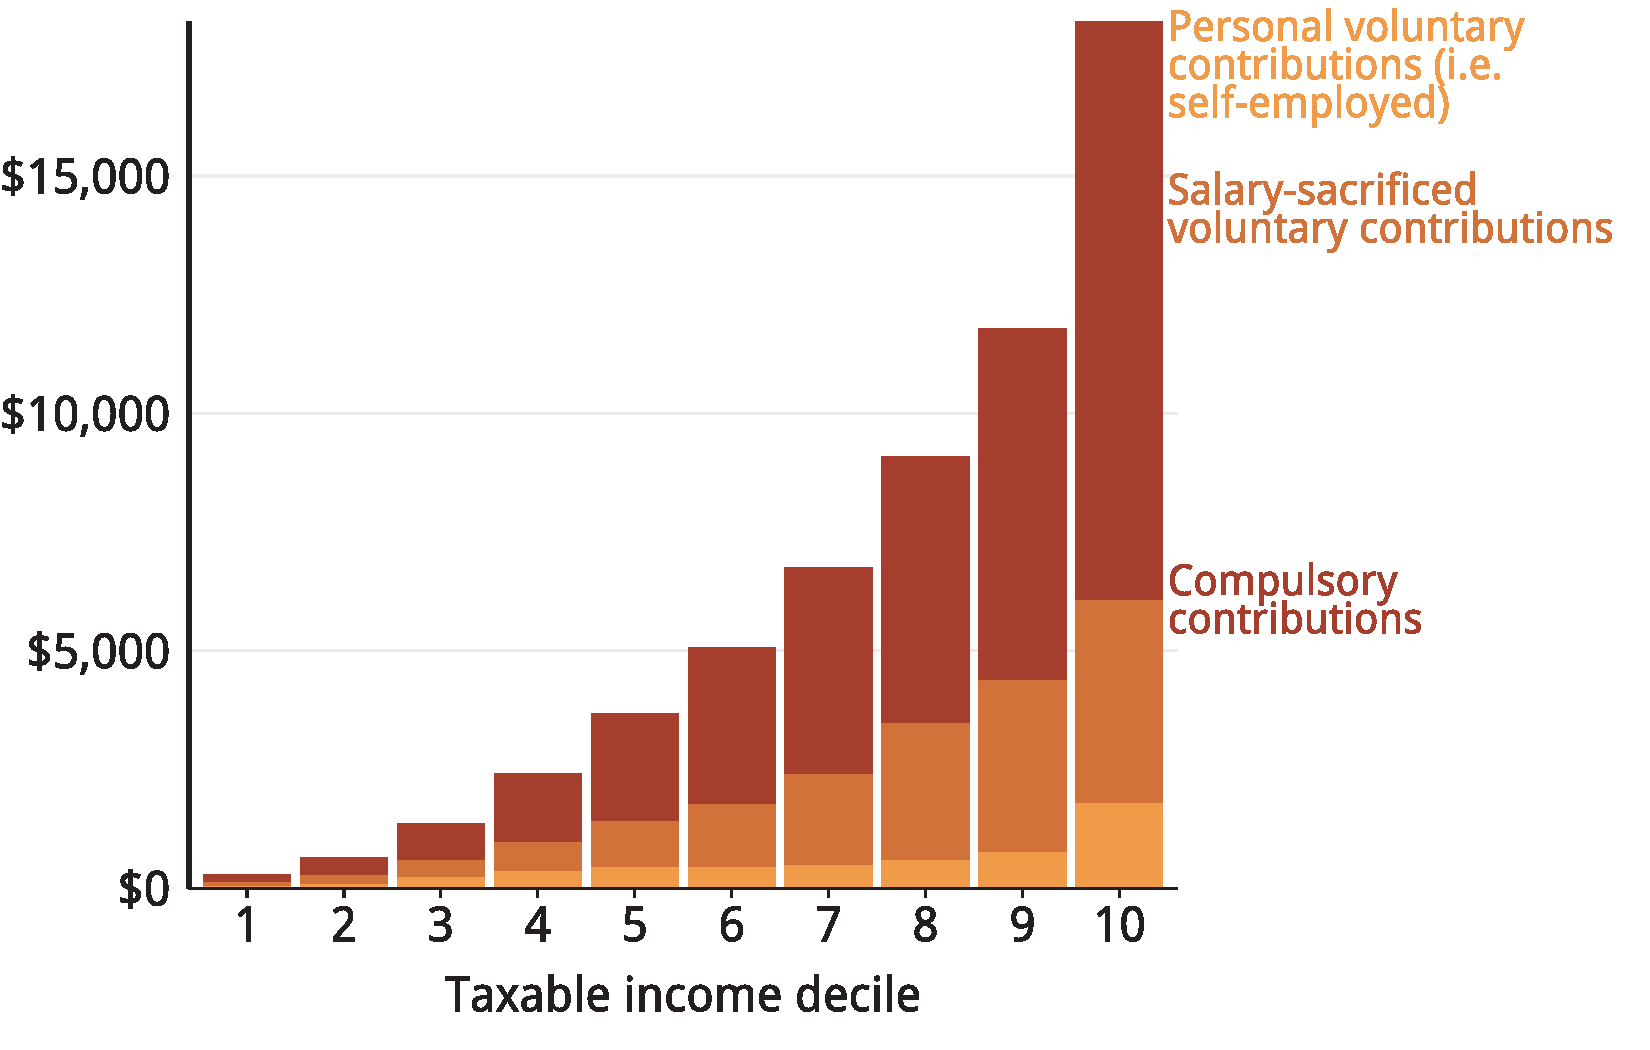
\includegraphics[width=\linewidth]{b5-super-atlas/Figure4-4-1.pdf}
\notes{2012-13 dollars. Excludes compulsory employer contributions beyond the Super Guarantee rate. Does not include post-tax super contributions. Taxable income deciles are for taxpayers aged 50 and over.}
\source{\textcite{ATO2015SampleFile1213}; Grattan analysis.}
\end{figure}

\section{Most voluntary contributions are made later in life and are unlikely to increase \emph{net} savings much\label{sec:SUPER-4-3}}
Over half of all pre-tax voluntary contributions are made by those in the top 20 per cent of income earners, and over half are made by those over 55 (\Cref{fig:SUPER-4-5}).\DEVIATION{} 

\begin{figure}[ht]
\captionwithunits{Voluntary pre-tax contributions are mostly made by those who are older and on high incomes}%
{Total voluntary pre-tax contributions 2012-13, by income decile and age}\label{fig:SUPER-4-5}
% 
\includegraphics[width=\columnwidth,page=23]{super-atlas/PPTX.pdf}
\centering
\includegraphics[height=0.6363\linewidth]{b5-super-atlas/pie-charts/Figure4-5Tikz-with-text.pdf}  % too wide
% 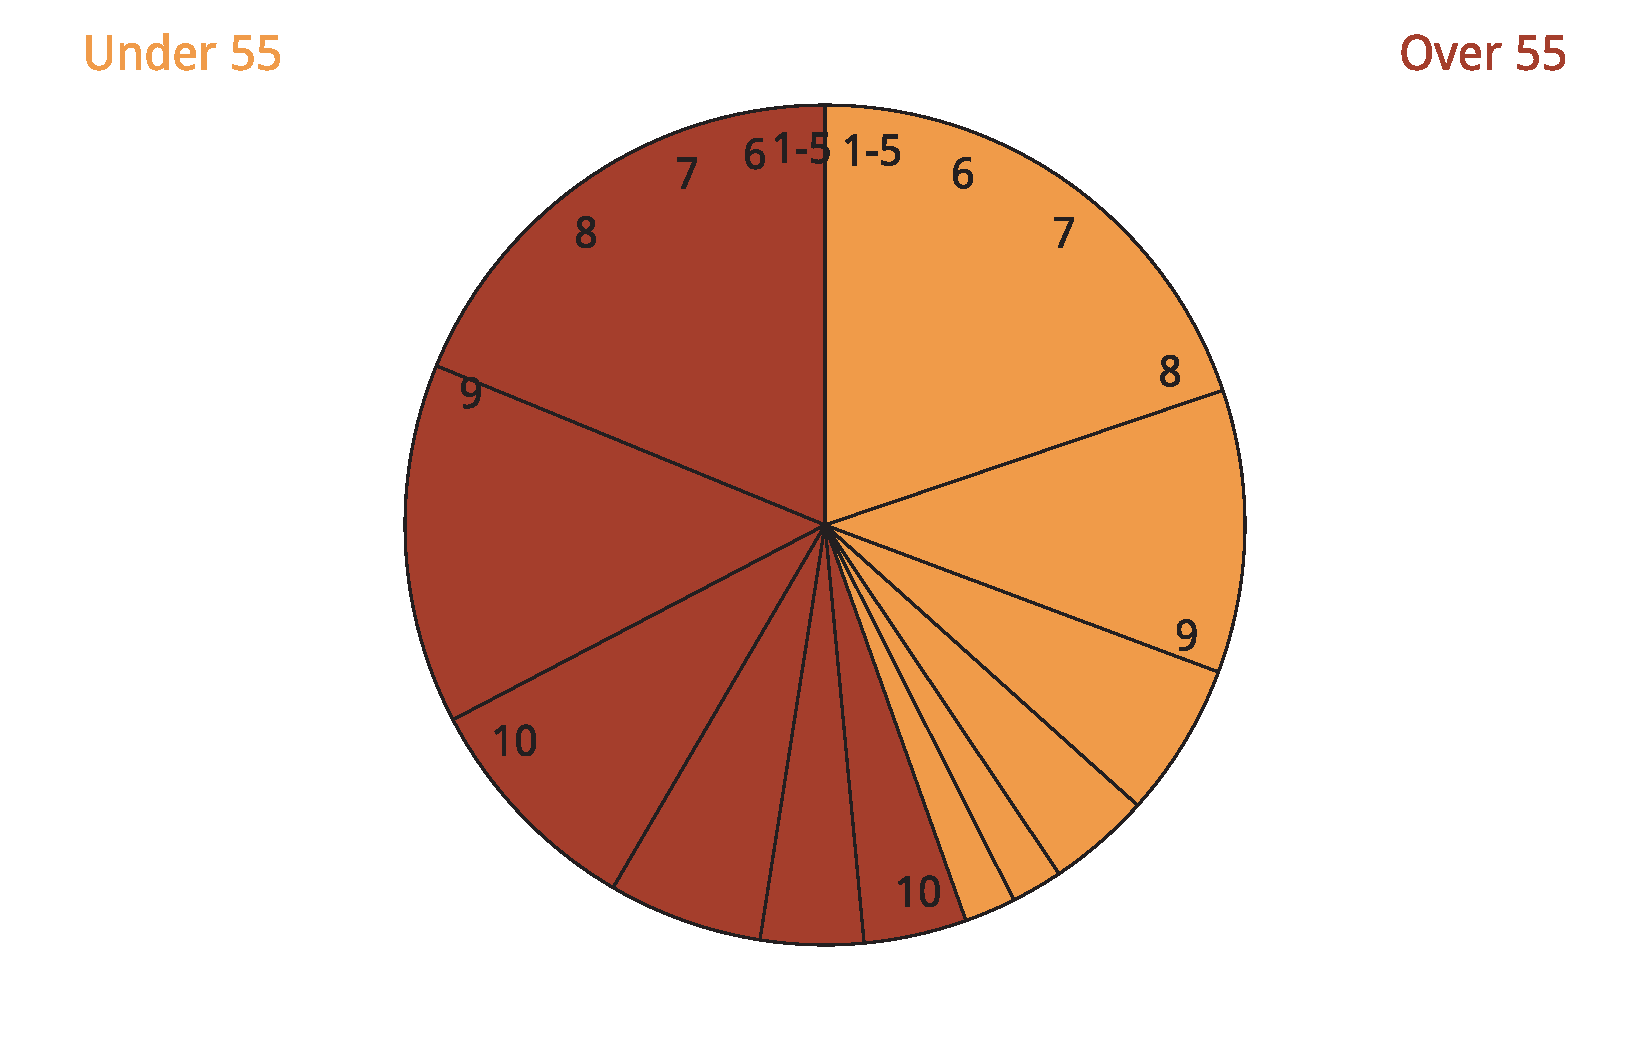
\includegraphics[width=\linewidth, trim = {0, 46pt, 0, 46pt}, clip]{b5-super-atlas/Figure4-5-1.pdf}
\notes{Includes reportable salary sacrifice contributions and contributions from post-tax income for which the taxpayer has claimed a tax deduction for 2012-13.}

\source{\gao\ \textcite{ATO2015Taxstats1213}.\hfill}
\end{figure}

Around 24 per cent of voluntary pre-tax contributions are made by those aged over 60 entitled to withdraw their contributions immediately, as shown in the more detailed analysis by age and income decile in \Cref{fig:SUPER-A-2}.

These super contributions do less to boost retirement incomes since they compound for a shorter period before retirement. Very few people under the age of 50 make material voluntary concessional contributions, even when they are in the top 10 per cent of income earners (\Cref{fig:SUPER-A-7}).

\section{People making large pre-tax contributions are unlikely to qualify for an Age Pension}
Only 12 per cent of taxpayers – about 1.6~million people make pre-tax contributions of more than \$10,000 in a year. Almost 1~million of these are in the top 10 per cent of income earners (\Cref{fig:SUPER-4-6}). Less than 5~per~cent of median-income earners make pre-tax contributions of more than \$10,000. By contrast, 79~per~cent of men (and 61~per~cent of women) in the top income decile contribute over \$10,000 (\Cref{fig:SUPER-A-7}). 

There are 163,000 women earning less than \$77,000 making pre-tax contributions of more than \$10,000. In contrast, there are more than 900,000 men earning more than \$77,000 that contribute more than \$10,000 a year from pre-tax income.

Most of these high-income earners need little help to provide for their own retirement. Often they are just making compulsory 9.5 per cent contributions, which will be more than \$10,000 if they earn more than \$105,000.

\begin{figure}
\captionwithunits{Few people other than high-income earners contribute over \$10,000 a year}%
{Number of individuals whose pre-tax contributions exceeded \$10,000, 2012-13}\label{fig:SUPER-4-6}
% 
\includegraphics[width=\columnwidth,page=24]{super-atlas/PPTX.pdf}
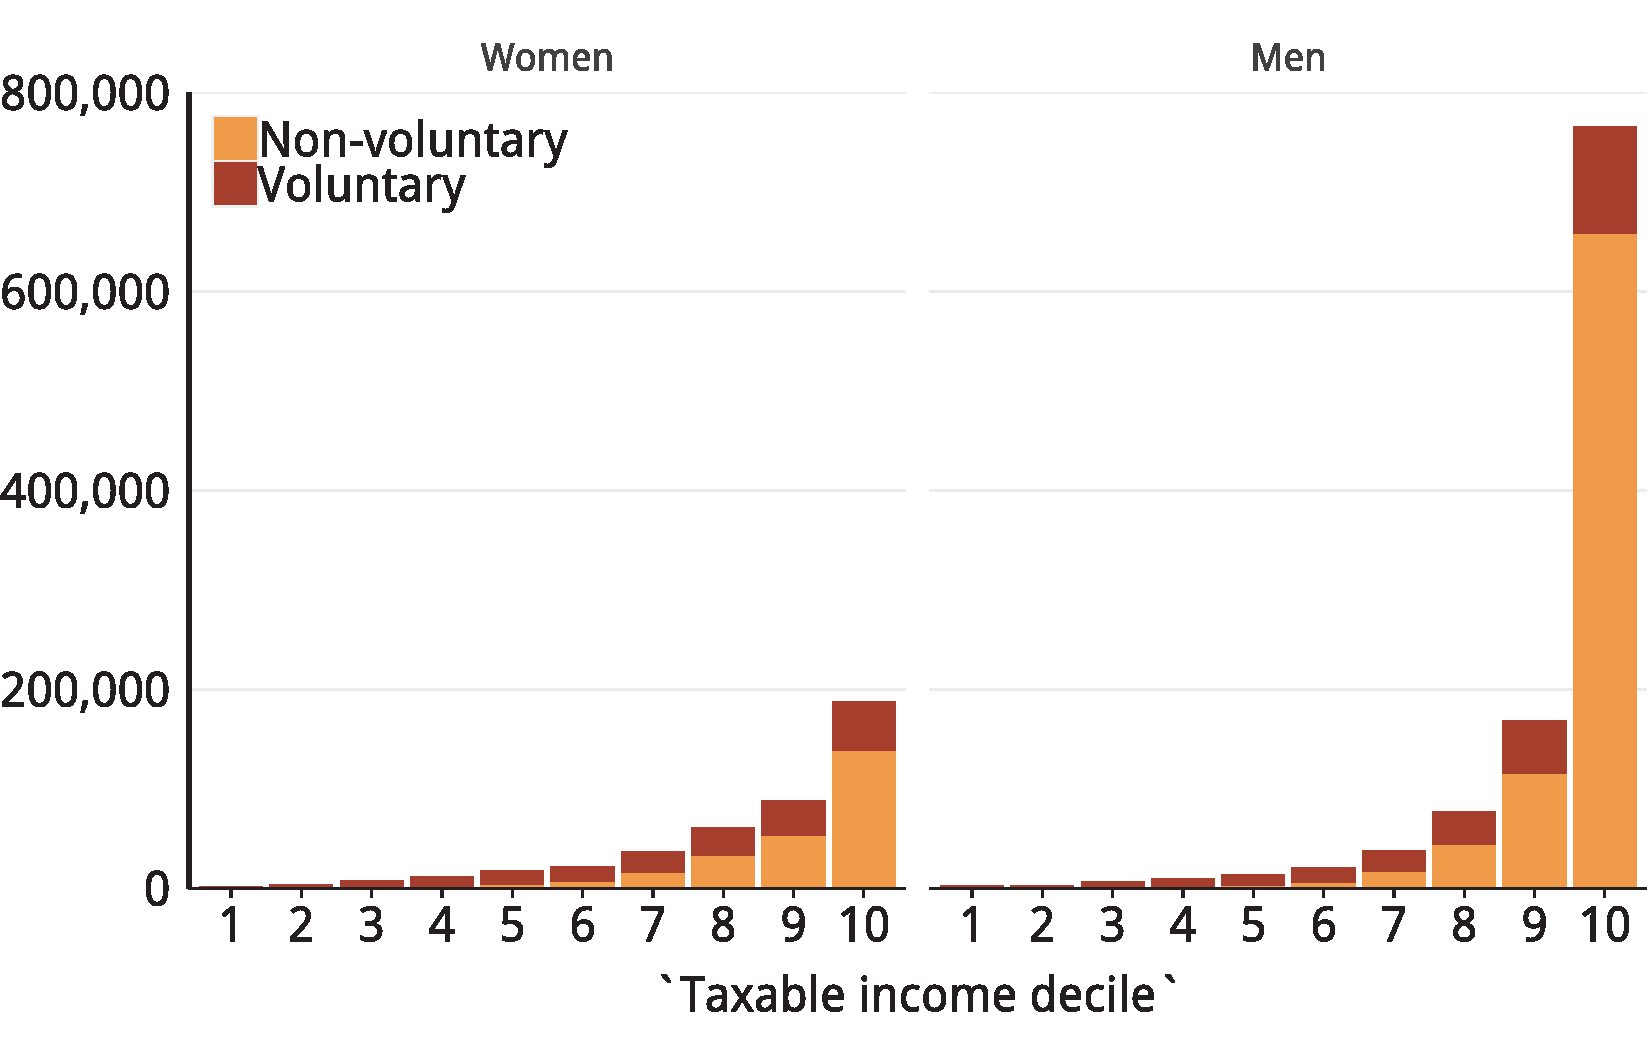
\includegraphics[width=\linewidth]{b5-super-atlas/Figure4-6-1.pdf}
\fnotes{fig:SUPER-4-6}{Compulsory Super Guarantee contributions estimated from salary and wage income; includes reportable salary sacrifice contributions and contributions from post-tax income for which the taxpayer has claimed a tax deduction. There were 1.27~million people in each taxable income decile in 2012-13.}

\source{\textcite{ATO2015SampleFile1213}; Grattan analysis.}
\end{figure}

Most \emph{voluntary} pre-tax contributions over \$10,000 are probably tax-planning measures rather than additional savings. High-income earners over 55 are much more likely to make voluntary pre-tax contributions, and to sacrifice a large part of their income when they do (\Crefrange{fig:SUPER-A-5}{fig:SUPER-A-6}). As shown in \Vref{fig:SUPER-4-7}, one third of all voluntary pre-tax contributions to superannuation over \$10,000 are made by people aged over~60. 

\begin{figure}
\captionwithunits{The bulk of voluntary concessional contributions over \$10,000 are made by those who are retired or close to retirement\label{fig:SUPER-4-7}}%
{Value of pre-tax voluntary contributions to superannuation in excess of \$10,000 in a year, 2012-13, \$2015-16 (by age)}
% 
\includegraphics[width=\columnwidth,page=25]{super-atlas/PPTX.pdf}
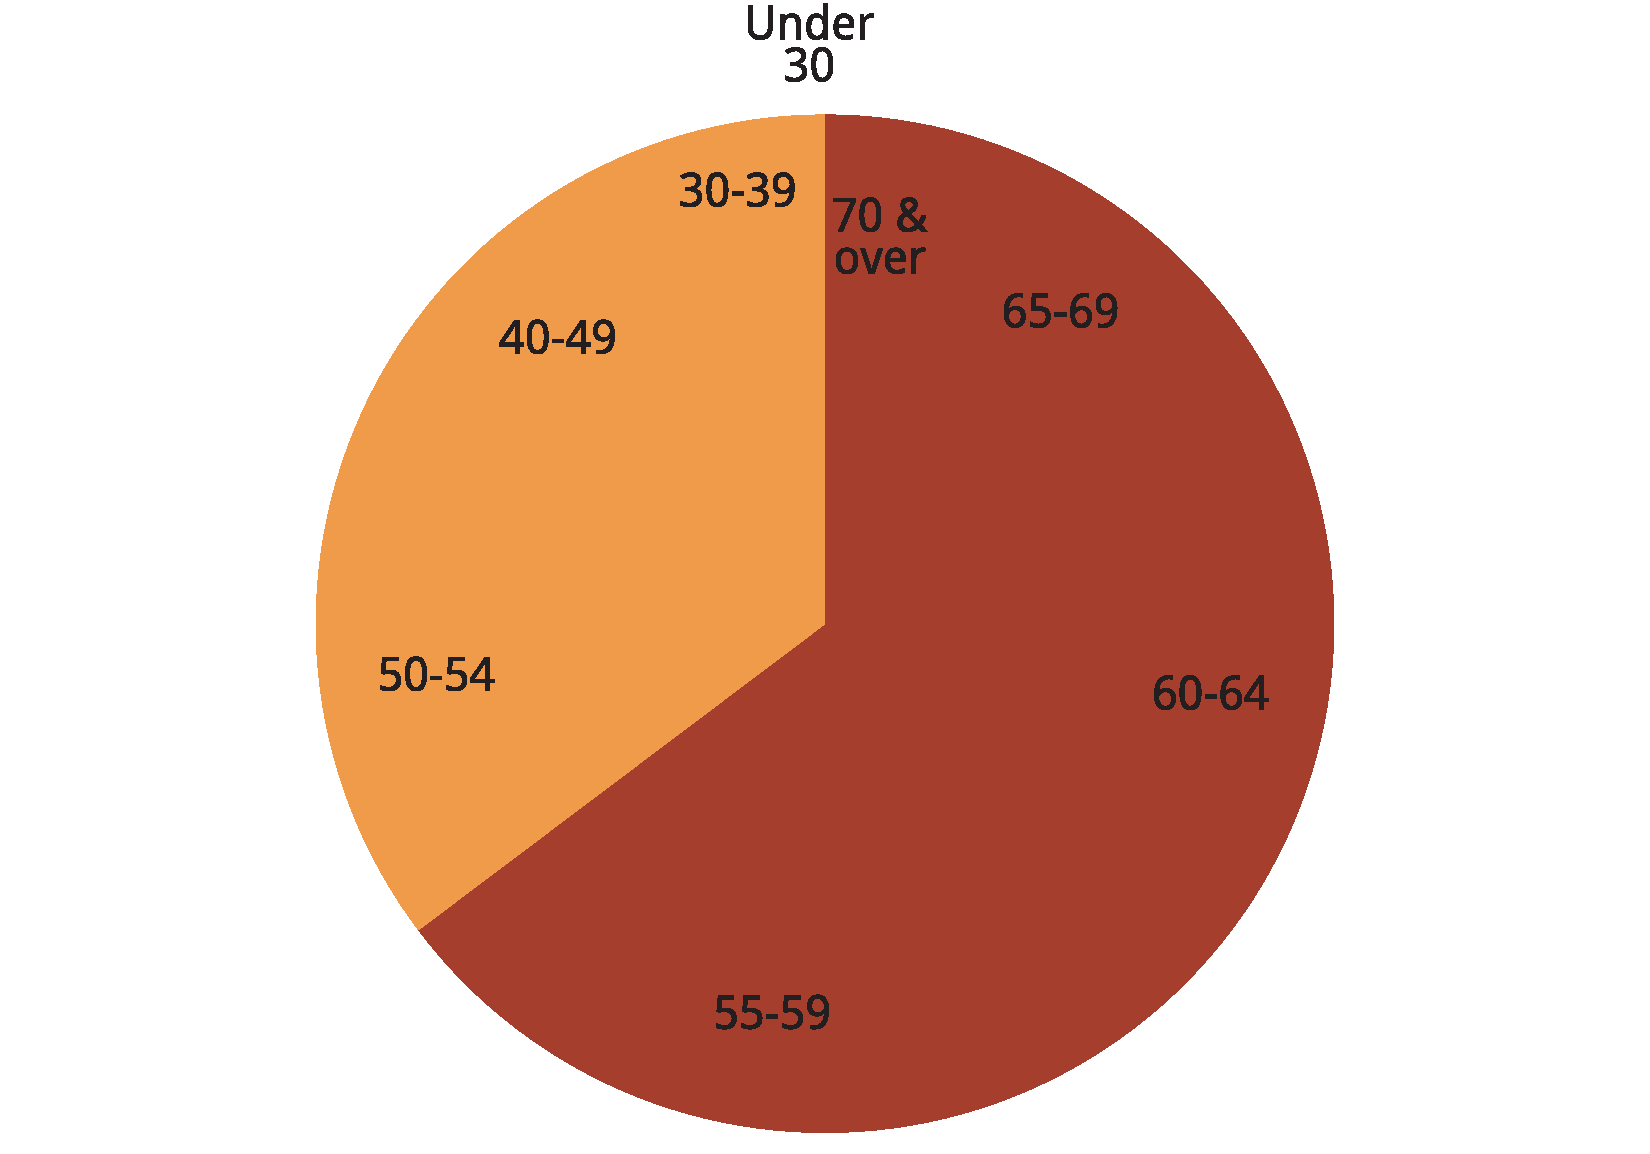
\includegraphics[width=\linewidth, clip]{b5-super-atlas/Figure4-7-1.pdf}
\source{\textcite{ATO2015SampleFile1213}; Grattan analysis.}
\end{figure}

Generally they can contribute from their pre-tax income, and then withdraw their superannuation immediately. By recycling wage income through their super fund in this way, middle- and high-income earners can continue to consume their income immediately while substantially reducing their tax liability. For workers aged between 60 and 64 years earning between \$65,000 and \$150,000, this strategy reduces the amount of tax paid by over \$5,000 (see \Cref{appendix:SUPER-B}). The tax benefits for workers aged 65 years and over are even larger.%
\footnote{Individuals aged 65 and over are also eligible for the Senior Australian and Pensioners Tax Offset (SAPTO), which can reduce their tax liability even further when recycling wage income through superannuation. \textcite{ATO2015-Beneficiary-tax-offset-sapto-calculator}} 





The ‘transition to retirement’ rules that allow workers between the age of 60 and 65 to access their super were originally designed to allow individuals to move from full-time to part-time work without reducing their incomes. Superannuation withdrawals would compensate for lower wages.\footcite{ASIC2015TransitionToRetirement}  However, recent evidence suggests that these rules are mainly used by high-wealth individuals to reduce their tax bills while they continue to work full-time.\footnote{Of the estimated 5 per cent of eligible Australians (workers aged between 55 and 65) who received transition to retirement pensions in 2011-12, the majority were working full time and were relatively wealthy (\textcite[][20]{ProductivityCommission2015SuperPolicyPostRetirement}). However, data on self-managed super funds suggest the transition to retirement pensions are used by around half of eligible SMSF members. This probably reflects how SMSF members tend to have more wealth and manage their superannuation more actively. \textcite[][144]{ProductivityCommission2015SuperPolicyPostRetirement}}  

Of course, some voluntary contributions made by over 60 year olds are not immediately withdrawn and consumed in this way. However, these voluntary contributions do not serve the purposes of superannuation if the person would have saved anyway, or if they would not in any case qualify for an Age Pension. More detailed analysis of annual contributions by age and taxable income is provided in \Cref{appendix:SUPER-A}.

\section{Superannuation contributions tax breaks could be reformed in a number of ways}
Various proposals have been made to target contribution tax  breaks better. We focus on three of these.

\DEVIATION{}
\begin{enumerate}
\item 
{\textbf{Reduce the concessional contributions cap to \$11,000}}\\
This would reduce the maximum amount that can be contributed annually to super from pre-tax income (the ‘concessional’ contributions cap) from \$30,000 (or \$35,000 for those over 50) to \$11,000. This could improve budget balances by around \textbf{\$3.9 billion} annually. This cap would still allow taxpayers earning 1.5 times average earnings to benefit from tax concessions for the full amount of super guarantee contributions made by their employer.\footnote{A worker with annual earnings of \$115,000 would receive SG contributions from their employer of \$10,925, at the current 9.5~per cent SG rate.}  The cap should be indexed to growth in wages (probably in \$1,000 increments) to prevent it eroding in real terms. The maximum superannuation contributions base would need to be reduced to \$115,000 so that workers are not compelled to make super contributions upon which they receive no tax concession.\footnote{Under the maximum superannuation contributions base, employers are obligated to make SG contributions on the first \$203,240 of employees’ wages. This equates to a maximum level of compulsory SG contributions of \$19,308 in 2015-16. The maximum super contributions base would be indexed to the same level each year as the concessional contributions cap.}  This policy is based on a proposal made in the Grattan Institute report \citetitle{DaleyMcGannonSavageEtAl2013BalancingBudgets}.\footcite[][32]{DaleyMcGannonSavageEtAl2013BalancingBudgets} \medbreak

\item 
{\textbf{Increase the tax rate on contributions to 30 per cent for those earning more than \$115,000}}\\
Those earning over \$300,000 already pay 30 per cent tax on contributions.\footnote{‘Division 293 tax’ imposes a 30 per cent tax rate on concessional super contributions from those whose earnings and super contributions exceed \$300,000 (\textcite{ATO2015HowisDiv293calculated}). It was introduced in 2012 (\textcite{Shorten2012}).}  This higher tax rate could apply to those on a lower income level, say \$115,000. This would improve budget balances by around \textbf{\$3.8~billion} annually.%
\FOOTNOTE{This figure has been updated since first publication.} %
 The income threshold from which a 30 per cent tax rate applies would be indexed annually to average weekly earnings so that the value of the super tax breaks is not eroded over time. This design takes further proposals from the Australian Labor Party to apply a 30 per cent tax on contributions for those earning more than \$250,000.\footcite{ALP2015FairerSuper} 

\item 
{\textbf{Tax contributions at marginal rates, less a 20 per cent discount}}\\
Taxpayers could contribute to superannuation at their current marginal tax rate, less a uniform 20 per cent rebate. We assume that the current cap of \$30,000/\$35,000 on concessional contributions remains in place.\footnote{At the time of the Henry Review, the cap was of \$25,000 or \$50,000 for people aged 50 or older (\textcite[][100]{HenryTaxReview2010}).}  This policy would remove the penalty for those on low marginal tax rates making super contributions by providing a top-up payment to their super account. This could improve budget balances by around \textbf{\$1.1 billion}, while also improving the super balances of those on low incomes.%
\footnote{Analysis for the Henry Review found that such a proposal would have a budget cost of \$4 billion\DEVIATION{} a year by 2017-18, but this assumed a simultaneous change that allowed an income earner to make two pre-tax contributions of up to \$30,000 each year, one to their own account and another to that of their partner. This costing also anticipated a higher cap of \$50,000 on the pre-tax contributions of those aged over 50: see \textcites{Treasury2010SuperAdditionalMaterial}[][95]{HenryTaxReview2010}.}  
This reform extends a proposal in the Henry Tax Review,\footcite[][102]{Treasury2010IGR}  recently taken up by Deloitte Access Economics,\footcite{Deloitte2015TaxReformSheddingLight}  to tax contributions at the taxpayer’s marginal rate, less 15 per cent.
\end{enumerate}

To mirror the benefit to low-income earners of the third proposal, the first two reforms could be supplemented by the retention of the Low Income Super Contribution beyond 2016-17 so that low-income earners are not disadvantaged when contributing to super. This would cost around \textbf{\$1~billion}.\footcite[][Table~2.16, p.~206]{Treasury2013PortfolioBudgetStatement1314}

A further option for reform would be to impose a lifetime cap on concessional contributions. However, this would further entrench the tax advantages for wealthy older workers, and encourage more tax planning rather than genuine increases in savings. The budgetary impact is also difficult to ascertain from publicly available data. 

Older workers who have already benefited from particularly generous superannuation tax breaks that are now closed would be even further advantaged by a lifetime cap relative to younger workers. Data on contributions may not be as reliable before 2003-04, and so contributions before then – mostly made by older workers – would not be included.\footnote{\textcites{SuperContrTaxRegs1997}{ATO2003}{ATO2008}{ATO2014g}{ATO2014h}} Furthermore, because records are limited, it would be a long time before many people reached the recorded lifetime cap on contributions, and so a lifetime cap would have little budgetary impact for many years.

A lifetime cap creates significant tax-planning opportunities. To maximise their superannuation tax breaks, taxpayers who have not used up their lifetime cap could sacrifice the entirety of their earnings. Such tax-planning is likely given how post-tax contributions are used already (\Cref{sec:SUPER-5-1}).\footnote{Tax planning opportunities with a lifetime cap would be worth less if all taxpayers received the same value tax break per dollar contributed to super, as would occur under the model put forward by the Henry Tax Review considered in \Cref{sec:SUPER-4-6}.}  The existing tax breaks, limited by annual caps, are more difficult to game, since to maximise contributions taxpayers must make contributions consistently every year over decades.  

Limiting annual contributions, or taxing them at a higher rate, would be fairer between generations, and would raise more revenue. An annual contributions cap would be a reasonable proxy for a lifetime cap since someone who has the capacity to make a substantial contribution over \$11,000 in any one year is likely to have a higher income over their lifetime (\Cref{sec:SUPER-3-4}).

Views differ on an appropriate cap. Deloitte has suggested a lifetime cap of \$580,000.\footnote{\textcite[][18]{Deloitte2015DynamicsofAusSuper} argued that after taking into account the timing of voluntary contributions, this would be sufficient to produce a retirement income from age 65 to the 75th percentile of life expectancy.} The Association of Superannuation Funds of Australia (ASFA) has suggested \$1~million, which amounts to \$850,000 after contributions tax.%
\footnote{\textcite[][39]{ASFA2015TreasurySubmission}. ASFA also proposes this lifetime cap would be accompanied by a (higher) annual cap on pre-tax contributions of \$45,000.}
Both these proposals fail to target superannuation at its purposes. A superannuation account the size of ASFA’s lifetime cap would be well above ASFA’s own benchmark of the amount a couple needs for an affluent retirement even after the Age Pension assets test takes effect in 2017 (\Vref{tbl:SUPER-2}). The ultimate value of an account of this size would be much higher than the sum of lifetime contributions, once investment returns on the account are added. A couple would be even better off if they both have superannuation accounts (as many do), or if they have savings outside owner-occupied housing and superannuation – as almost all do when they have superannuation savings of this size (\Vrefrange{fig:SUPER-3-2}{fig:SUPER-3-3}). 

Other policy variations include an annual cap on pre-tax contributions, with an ability to roll over some portion of any unused cap for use in future years. This would create more tax planning opportunities than an annual cap, and fewer than a lifetime cap.\footcite[][18]{Mercer2015SubmissionToReThink}  However, such an approach would add further complexity to the superannuation system, particularly when there is little evidence that an annual cap on pre-tax contributions would in fact restrict many low and middle income earners from making ‘catch up’ super contributions (\Cref{sec:SUPER-4-3}).

\section{Reducing the maximum concessional contribution would be the best reform overall\label{sec:SUPER-4-6}}
As discussed above at \Cref{sec:SUPER-3-9}, reform should aim to minimise tax breaks that don’t serve the policy purposes of superannuation, maximise tax breaks that do, minimise the budgetary cost, and be administratively workable.


The first option for reform – reducing the concessional cap to \$11,000 – provides the best balance amongst these considerations, as summarised in \Vref{tbl:SUPER-5}, and elaborated below.

\begin{table}[p]
% Needs work.
\begin{minipage}[t][0.95\textheight]{\linewidth}
\caption{Assessment of concessional contribution reform options\label{tbl:SUPER-5}}
\renewcommand{\arraystretch}{2}
\begin{tabularx}{\columnwidth}{>{\raggedright\itshape\arraybackslash}p{0.16\linewidth}RRR}
\toprule 
% \barl Principles \earl & \barr Reduce\\ concessional\\ contributions\\cap to \$11,000 \earr & %
% \barr Increase tax on\\ contributions\\ to 30\%\ for\\ those earning \\ > \$115,000\earr & \barr Tax contribu-\\tions at\\marginal tax rate\\ less 20\%\earr \\
\tblHeadVCL{Principles} & \tblHeadVC{Reduce concessional contributions cap to \$11,000} & %
\tblHeadVC{Increase tax on contributions to 30\% for those earning >~\$115,000} & 
\tblHeadVC{Tax contributions at marginal tax rate less 20\%} \\
\midrule
    Minimise tax breaks that don’t serve policy purpose & Substantial reductions in tax breaks above 90th~percentile & Minimal tax break~for~95th percentile; large tax break for 99th~percentile & Reduce tax break~for~95th percentile, large tax break for 99th~percentile \\
    Maximise tax breaks that do serve policy purpose & Maintain incentives for 90th percentile & Little incentive for 90th percentile & Slightly reduced incentives for 80th and 90th percentile \\
    Equity & Reduce tax breaks for top 10\%; only helps lower income if reintroduce LISC & Reduce tax breaks for top 10\%; only helps lower income if reintroduce LISC & Increases progressivity of entire super system \\
    Budgetary impact & \$3.5 billion & \$3.8 billion & \$1.1 billion \\
    Administrative issues &  \begin{tabular}[t]{>{\raggedleft}p{\linewidth}} Builds on\\ existing\\ procedures \end{tabular}& \begin{tabular}[t]{>{\raggedleft}p{\linewidth}} Builds on\\ existing\\ procedures \end{tabular} & \begin{tabular}[t]{@{}>{\raggedleft}p{0.95\linewidth}@{}} Requires significant systems changes\end{tabular} \\
    \bottomrule
\end{tabularx}
\end{minipage}
\end{table}%

\subsection{Targeting tax breaks at those need them}
All three proposals would reduce the super contribution tax breaks for high-income earners, as shown in \Vref{fig:SUPER-4-8}. 

\begin{figure}
\captionwithunits{Lowering the concessional threshold would mainly affect the highest income earners}%
{Contributions tax concession per taxpayer in 2012-13 (2015-16 dollars)}\label{fig:SUPER-4-8}
% 
\includegraphics[width=\columnwidth,page=26]{super-atlas/PPTX.pdf}

\includegraphics[width=\linewidth]{b5-super-atlas/Figure4-8-1.pdf}
\fnotes{fig:SUPER-4-8}{For proposals to change tax rates on contributions, we assume a concessional contributions cap of \$30,000 remains in place (\$35,000 for over 50s); \$11,000 cap proposal assumes Division 293 tax remains in place for those earning more than \$300,000; a taxpayer earning more than \$115,000 is assumed to make pre- and post-tax total contributions of 9.5 per cent of their taxable income. Estimates of tax concessions do not include tax savings of avoiding the Medicare Levy or Temporary Budget Repair~Levy.}

\source{\textcite{ATO2015Taxstats1213}; Grattan analysis.}
\end{figure}

\begin{figure}
\captionwithunits{All income levels would have ample incentives to save in superannuation under the reforms proposed}%
{Real effective tax rate on long-term earnings from superannuation savings}\label{fig:SUPER-4-9}
% 
\includegraphics[width=\columnwidth,page=27]{super-atlas/PPTX.pdf}
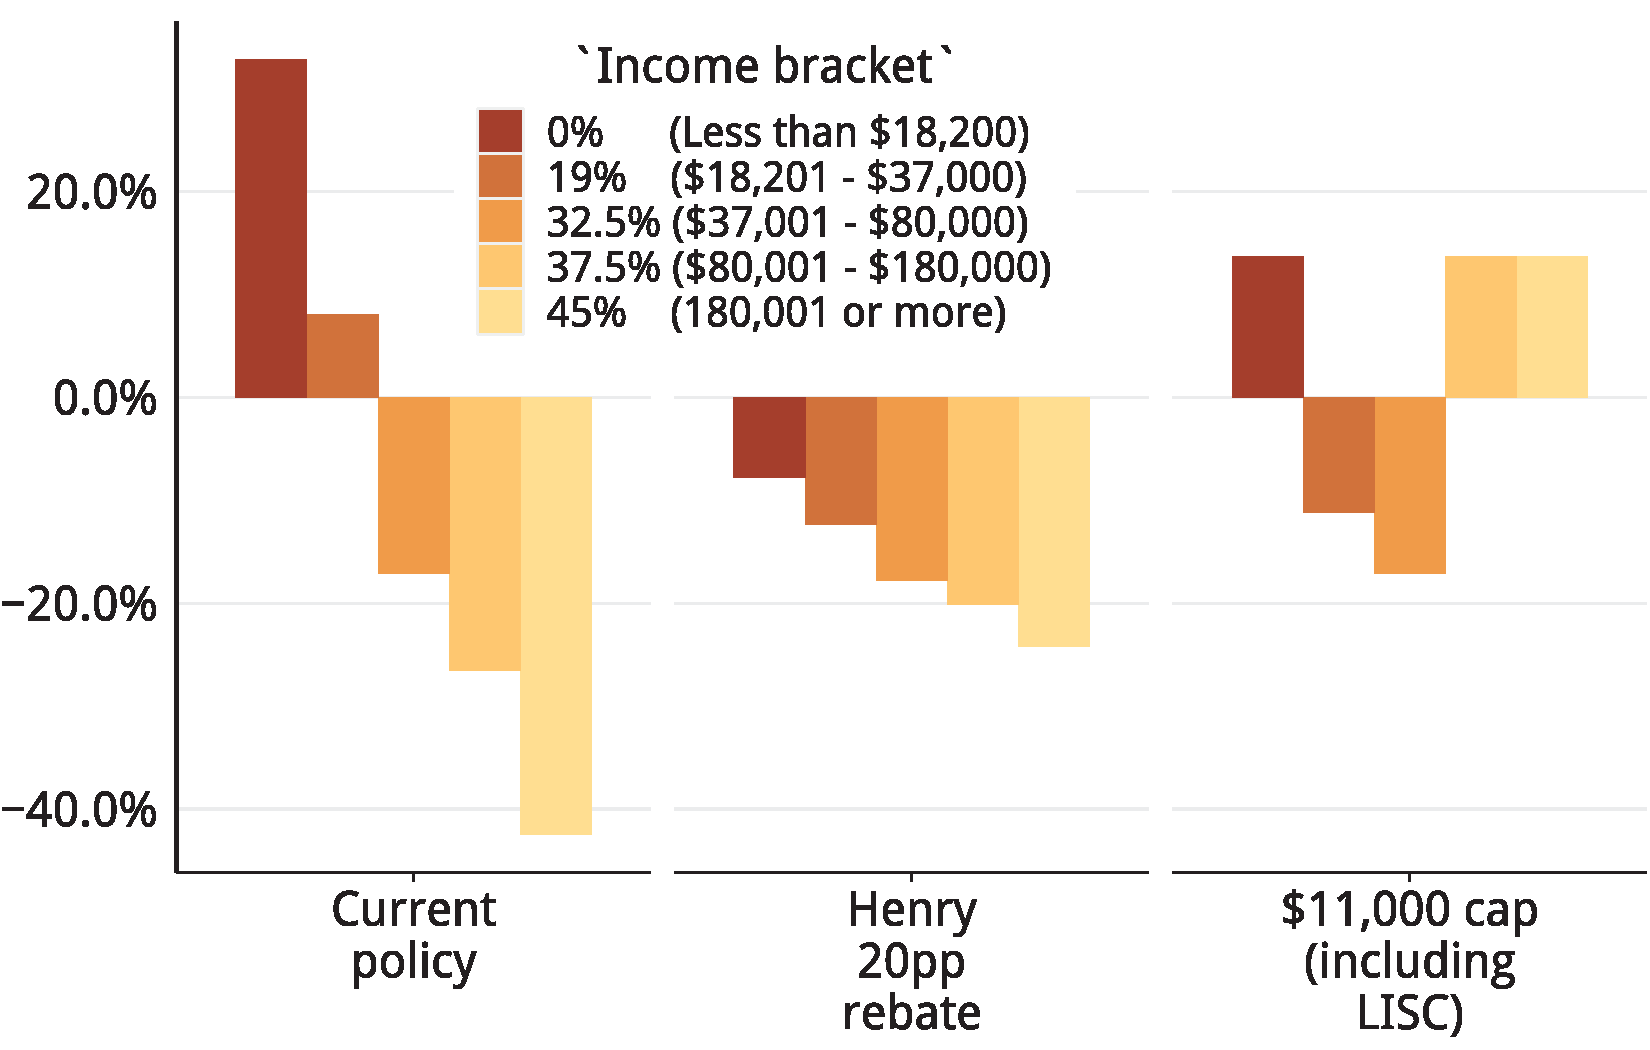
\includegraphics[width=\linewidth]{b5-super-atlas/Figure4-9-1.pdf}
\notes{Assumptions as for \Cref{fig:SUPER-4-8}, except that the proposed concessional contributions cap of \$11,000 assumes a LISC of up to \$530 for those earning up to \$37,000, so that a contribution is made to all wage earners equivalent to the 9.5 per cent Superannuation Guarantee rate. Calculations of the post-tax baseline include the Medicare Levy only for taxpayers with incomes over \$37,000. Real effective tax rates are defined as per the note to \Cref{fig:SUPER-2-3} and set out in \Cref{appendix:SUPER-C}.}
\end{figure}

Capping pre-tax contributions at \$11,000 would reduce the tax breaks for very high-income earners more than the other proposals. This option would also have smaller impact on the contributions of those in the 8th and 9th~deciles of taxpayers – those who are likely to be on the threshold of qualifying for a part Age Pension.\footnote{The value of the contributions tax break would fall more than shown in \Cref{fig:SUPER-4-8} for some workers whose employers contribute more than the 9.5~per cent Super Guarantee rate under awards or agreements, so that their total contributions are more than the \$11,000 cap. Government would need to consider whether to raise the \$11,000 cap if the Superannuation Guarantee rises from 9.5~per cent to 12~per cent, as currently legislated.} 

The Henry Review proposal to tax contributions at marginal tax rates, less a 20 per cent discount, would deliver increases in super to the bottom 70 per cent, but would also deliver more super to the very highest income earners. The alternative version of the Henry Review proposal put forward by Deloitte, with a 15 per cent discount, would help the bottom 30 per cent, but would leave middle-income earners worse off than they are today. 

Even if the proposals made later in this paper were adopted, there would still be substantial incentives for high income earners to save via superannuation, even if they do so from post-tax rather than pre-tax income. As \Vref{fig:SUPER-4-9} shows, the effective tax rate on earnings would still be low. Compared to the alternatives, superannuation would remain a highly attractive vehicle for the long-term savings of high-income earners (\Cref{fig:SUPER-2-3}).%
\enlargethispage*{0.5\baselineskip}\enlargethispage{0.5\baselineskip}

\subsection{Increasing equity}
All of the proposals would reduce the superannuation tax breaks for the top 10~per cent of taxpayers. The Henry proposal – or a variant on it – is the only proposal examined that would improve the value of superannuation tax breaks to low-income earners: it proposed to reduce the tax rate on their contributions to under 15 per cent. In this respect it is similar to the Low Income Superannuation Contribution Scheme. In addition, the Henry proposal would also top up a low-income earner’s super account if the rebate were higher than their marginal personal income tax rate.\footnote{Individuals with taxable incomes of below \$37,500 face marginal tax rates of up to 19 per cent, plus the Medicare Levy of up to 2 per cent.}\

However, it is unclear that topping up superannuation accounts is the best way to improve retirement incomes for the poor. Those on low incomes accumulate relatively less superannuation, and casual employment with multiple employers often leads to multiple small superannuation accounts. Administration fees can eat up most or all of the balances. Although beyond the scope of this report, it is possible that government funds would have more impact if they simply contributed to increasing the full Age Pension or Rental Assistance for pensioners.

Some argue that the Henry proposal is fairer because it provides an equal tax break to all taxpayers. However, that this argument is used only demonstrates how far superannuation has drifted from its purposes. Superannuation should not simply deliver an equivalent tax break to all taxpayers. It should deliver a tax break that serves the purposes of encouraging savings that will supplement or replace the Age Pension. Tax breaks for high-income earners, equivalent or otherwise, don’t serve this purpose.

\subsection{Budgetary impacts}
The three proposals would each have similar budgetary impacts, as shown in \Vref{fig:SUPER-4-10}.%
\enlargethispage*{0.5\baselineskip}\enlargethispage{0.5\baselineskip}

These estimates of budgetary savings are not affected much by behavioural change.\footnote{This is consistent with \textcite{Treasury2015TES2014}, which suggests behavioural change will be limited: the difference between Treasury’s ‘revenue foregone’ and ‘revenue gain’ estimates of the cost of contributions tax breaks is just 5 per cent.}  All of the proposals effectively limit the ability to save (or spend) from pre-tax income. There are no obvious alternatives that would allow income earners to save from pre-tax income, and so pay less income tax up front on savings. Even in the long-term, behavioural change will have little impact on budget outcomes. High-income earners affected by the proposals are unlikely to reduce savings rates much (\Cref{sec:SUPER-3-2}). And high-income earners are unlikely to find other investment vehicles for savings on which they pay less tax than superannuation (\Cref{fig:SUPER-2-3}). 

\begin{samepage}
At the margins, these changes might lead to some increase in high-income earners investing more in owner-occupied housing or geared investor housing rather than financial assets. Rather than detracting from the case for superannuation reform, this reinforces the importance of reforming property taxes,\footcite{DaleyCoates2015PropertyTaxes}  negative gearing, and capital gains tax rules.\footnote{\textcites{DaleyMcGannonSavage2013BudgetPressures}{DaleyWood2016NG}.}
\end{samepage}


Nor would these budgetary savings be offset by large future increases in Age Pension spending. All of the proposals would primarily reduce the superannuation tax breaks for the top 10 per cent of taxpayers. As noted in \Cref{sec:SUPER-3-5}, the top 10 per cent of income earners can expect to receive little or no Age Pension payments over their lifetimes, but benefit the most from tax breaks on superannuation contributions. Therefore reducing the value of superannuation tax breaks to this group will have little impact on future Age Pension expenditure. The Henry proposal – with a 15 per cent offset to marginal tax rates – would result in modestly larger increases in future Age Pension spending since it reduces the value of contributions tax breaks to middle-income earners.

\begin{figure}
\captionwithunits{Reforms to tax concessions on super contributions could significantly help the budget bottom line}%
{Revenue gain from reform options, (2015-16 billions)}\label{fig:SUPER-4-10}
% \includegraphics[width=\columnwidth,page=28]{super-atlas/newPPTX.pdf}
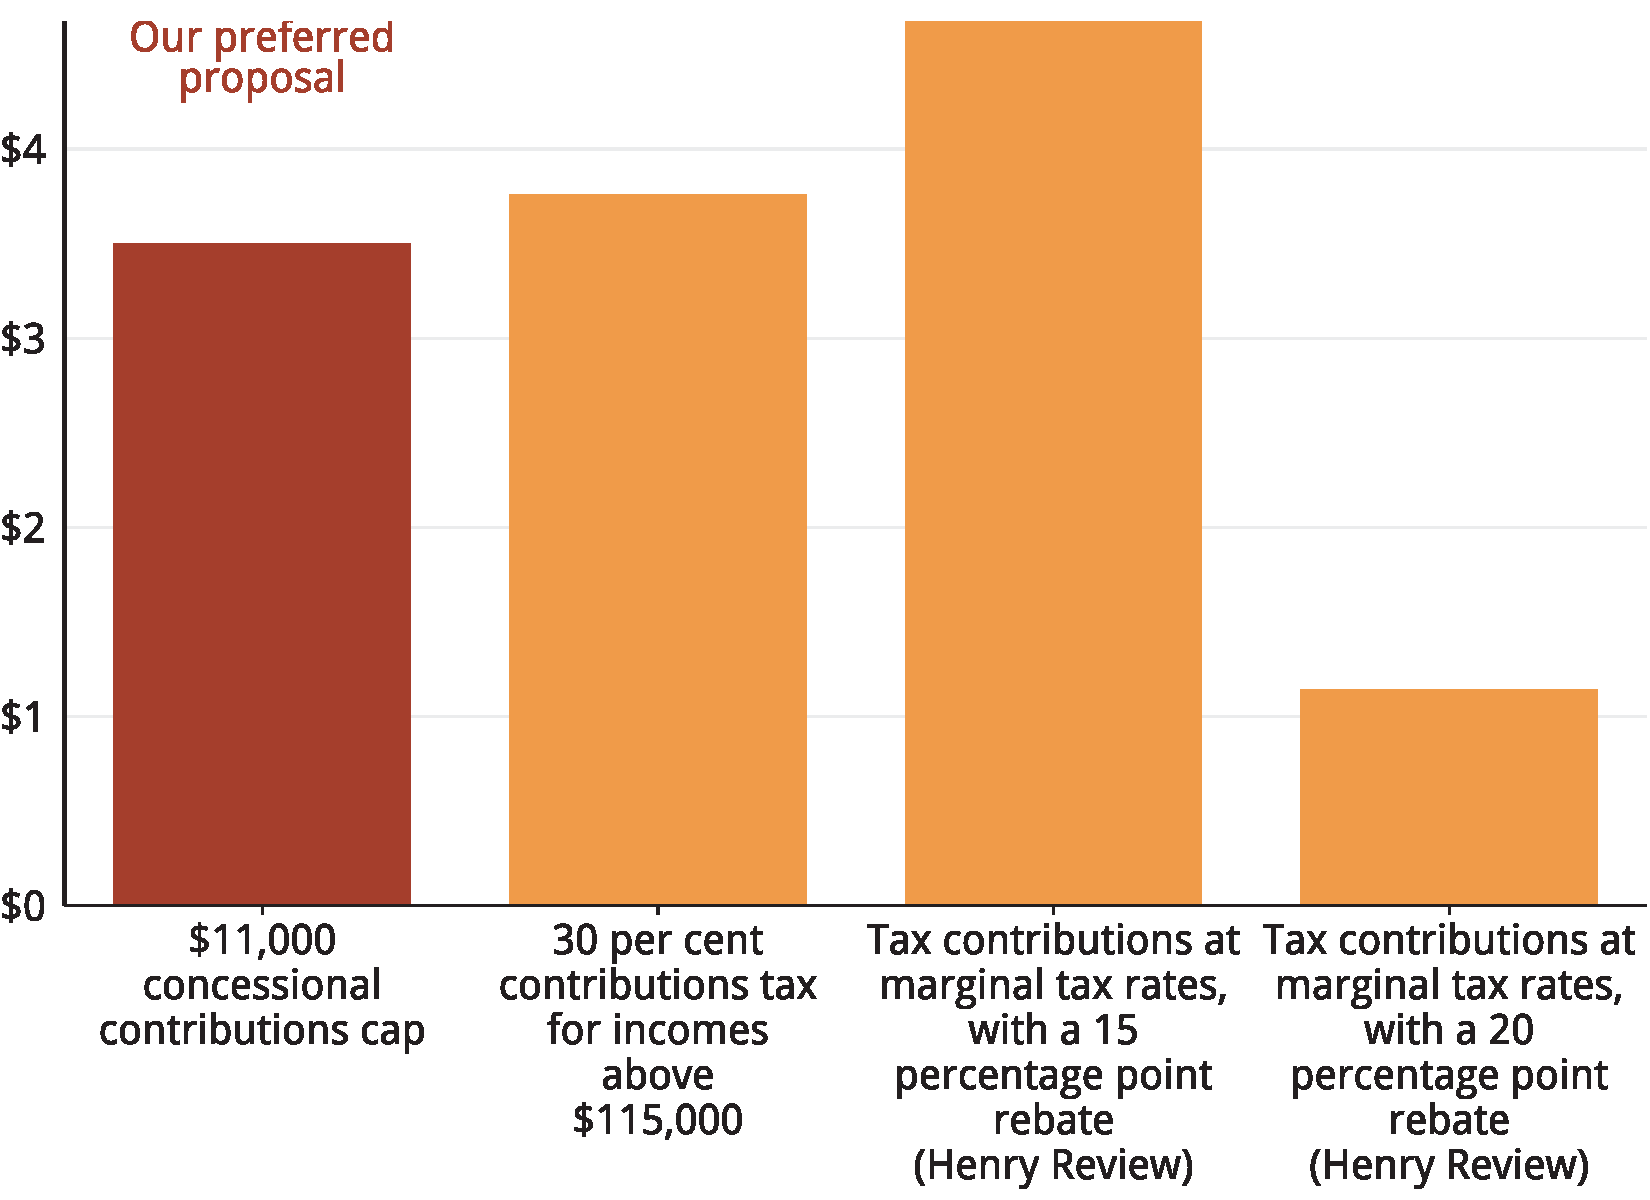
\includegraphics[width=\linewidth]{b5-super-atlas/Figure4-10-1.pdf}
\notes{As per \Cref{fig:SUPER-4-8}. \textcite{Deloitte2015TaxReformSheddingLight} estimate a slightly higher budgetary gain of \$6 billion per year from taxing contributions at a 15 percentage point discount to marginal rates of tax.}

\source{\textcite{ATO2015SampleFile1213}; Grattan analysis.} 
\end{figure}

The budgetary impacts illustrate the advantages of targeting super tax concessions at their policy purpose.\DEVIATION{Too long a para} 

The original Henry proposal, advocated by many industry group submissions to the Commonwealth Government’s tax reform process, would tax contributions at marginal tax rates less a 20 per cent discount. We estimate that this would do relatively little for the budget bottom line, saving just \$1.1 billion in 2015-16. It would do little for equity – indeed it marginally increases the tax break for those earning more than \$300,000 a year, whose contributions are currently taxed at 30 per cent under Division 293 tax.\footnote{The Henry proposal could be combined with a tighter cap on concessional contributions to reduce the tax breaks available to high-income earners. However, this would still entail the administrative challenges detailed below.}  The modified Henry proposal of taxing contributions at marginal tax rates less a 15 per cent discount adds much more to the budget bottom line, but at a cost to the super balances of middle-income earners. 

By contrast, capping pre-tax contributions at \$11,000 provides large budgetary savings, with little impact on the super balances of middle-income earners. 

\subsection{Administrative issues}
The first two proposals do not raise substantial administrative issues. Reducing the cap for pre-tax contributions, or reducing the income from which higher tax is paid on contribution, both build on existing features of the superannuation system. More taxpayers would be affected by these rules, but administrative arrangements would not change, including for defined benefit schemes.\footnote{Defined benefit superannuation schemes are already required to report the notional taxed contributions for each fund member in order to administer the annual cap on pre-tax super contributions (\textcite{ATO2015DefinedBenefitFundsNotionalTaxedContributions}). Such notional contributions are subject to Division 293 tax where the taxpayer meets the income test (\textcite{ATO2015AssessingYourDiv293TaxDebt}).}  The Henry proposal, however, would require substantial new arrangements.

Reducing the cap for pre-tax contributions would affect about 1.6 million taxpayers, assuming no change in behaviour (\Cref{fig:SUPER-4-6}). In reality, the number affected would be less than this: some people will respond to the changes in tax rates by dropping their contributions to the cap and redirecting their savings elsewhere. It is unlikely that this would ‘overwhelm the ATO’,\footcite{Sloan2015a}  which already routinely collects information from super funds on all super contributions by all taxpayers, and requires those who have contributed more than the existing caps to pay more tax either from their post-tax income, or from their superannuation fund.

Levying a higher tax rate on the super contributions of those earning more than \$115,000 would affect about 1.45~million taxpayers. Again the ATO would require these people to pay more tax either from their post-tax income, or from their superannuation fund.

The Henry model would raise significant new administrative issues.

The best mechanism we have identified for implementing the Henry model would shift responsibility for paying contributions taxes. Instead of super funds paying tax of 15 per cent on all pre-tax contributions received,\footnote{Super funds pay 15 per cent tax on all super contributions financed from the pre-tax income of the super fund member. However, super funds do not pay tax on any contributions financed from post-tax income, as this income has already been subject to full rates of personal income tax. }  employers would withhold tax on contributions paid at the marginal rates applicable for that employee,\footnote{For employees with multiple employers, these would be based on the schedules in place for PAYG tax collections. \textcite{ATO2015WhenYouHaveIncomeFromTwoPayers}.}  less the rebate, through the PAYG tax system. Discrepancies between an employee’s presumed income and their actual taxable income would be reconciled through tax returns. Employees would have an option to deduct unpaid tax from their super fund balance (as they do with Division 293 tax and extra tax on contributions in excess of the concessional cap). Legislation would clarify that contributions to super specified in awards or employment agreements would be deemed to include the tax paid by employers.

However, this would require significant systems reform. Many employers operate one system for regular earnings and PAYG tax payments, and another system for superannuation payments. The earnings PAYG system does not necessarily have information about the amount of superannuation contributed (which can vary depending on awards, individual employment agreements, and salary sacrifice arrangements).\footnote{The administrative issues are discussed further in \textcite{Mercer2015SubmissionToReThink}.} 

Even where salary and superannuation contributions systems are linked, there would be transition costs. For each employee, the employer would need to change the amount contributed to the superannuation fund (depending on the employee’s tax rate), and increase the amount forwarded to the ATO. 

While the Henry reforms were originally designed to deliver a net increase in super contributions, they could instead be designed (as we have assumed) to deliver no change to take-home pay, no change to super contributions before tax, but with changes (depending on the employee’s total earnings) to the amount of contributions tax paid. The positive budget impact we have calculated implies that net super contributions (after tax) would be lower. Superannuation funds might advocate that the increased tax be paid from take-home pay rather than super contributions. However, this would require substantial changes to a wide range of awards and individual contracts that specify how much should be contributed to superannuation before contributions tax, and add to the administrative complexity of the transition.

The Henry model would have some benefits for superannuation funds. Currently, funds must know whether contributions are taxable or non-taxable as they are received. Under the recommendation, funds would treat all contributions in the same way, making the system easier for them to administer.

\section{Transitional issues are straightforward}
Changing the taxation of contributions inherently raises few transition issues. By definition it only affects contributions that have not yet been made.

The proposals discussed in this chapter affect people who are yet to retire. High-income earners aged 50 and over will be affected most because they would otherwise receive large tax concessions in the medium term. In the long term, the changes would apply equally to future generations when they approach the end of their working lives. Delaying reform increases the implicit cost to younger households that pick up the tab for tax breaks that are likely to be changed before they benefit from them.\footcite{DaleyWoodWeidmannEtAl2014}

\chapter{Total super contributions} 
Post-tax super contributions are designed to allow individuals (such as those with broken work histories) to make top-up payments to a superannuation fund. Australians made \$33.6 billion in post-tax super contributions in 2012-13, about three quarters of all voluntary contributions (\Cref{fig:SUPER-4-1}). Clearly superannuation is an attractive destination for earnings even when contributions are made from post-tax income. 

In practice, many post-tax super contributions are motivated by tax-planning objectives rather than a need to build a reasonable balance after a broken work history. About 60 per cent of post-tax contributions are made by those aged over 60. Most of these contributions must be the movement of existing savings from other vehicles into superannuation, rather than additional savings for retirement.\footnote{About 30 per cent of those aged between 60 and 70 make post-tax contributions, contributing an average of \$40,000 each (\Cref{fig:SUPER-A-11}). If these contributions are from earnings, then they would be in addition to \$35,000 of pre-tax contributions. Average taxable incomes for this group are around \$50,000 (\textcite{ATO2015SampleFile1213}), and less than half are still in paid work (\textcite[][58]{ProductivityCommission2013AgeingAustralia}.}  As the Financial System Inquiry noted, many high-income earners can make large post-tax super contributions so that they pay less tax on the earnings on these savings, with no loss of flexibility once they begin to draw a retirement income stream.  They are also able to avoid inheritance taxes that are potentially payable on superannuation balances.

Consequently, the existing cap on annual post-tax contributions of \$180,000 – or \$540,000 over three years\footnote{Individuals can ‘bring forward’ three years of their pre-tax cap entitlement to make pre-tax contributions of up to \$540,000 in a single year (\textcite{ATO2015SuperContr--too-much-super-can-mean-extra-tax}.} – is far too high.  It should be reduced to a lifetime limit on post-tax contributions of no more than \$250,000 to provide a better balance between allowing for broken work histories and limiting tax planning. 

\section{Non-concessional contributions are mostly made by those who provide for their own retirement anyway}\label{sec:SUPER-5-1}
Unsurprisingly, high-income earners and those who are older are more likely to make non-concessional contributions, and make very large contributions when they do (\Vref{fig:SUPER-A-11}). Over three quarters of post-tax contributions are made by people aged over 55 (\Vref{fig:SUPER-5-1}). 

Most of these post-tax contributions are made by those who already have large super balances, rather than by those who are ‘catching up’ (\Vref{fig:SUPER-5-2}, and for more detail see \Vref{fig:SUPER-A-10}). Only 1.2 per cent of taxpayers have total super account balances of more than \$1 million, yet they account for 26 per cent of all post-tax contributions. The 70 per cent of taxpayers with super balances of less than \$100,000 account for just 9 per cent of post-tax contributions.  

\begin{figure}
\captionwithunits{Voluntary post-tax contributions are mostly made by those who are older and on high incomes\label{fig:SUPER-5-1}}%
{Percentage of voluntary post-tax contributions, 2012-13}
% 
\includegraphics[width=\columnwidth,page=29]{super-atlas/PPTX.pdf}
\includegraphics[width=\linewidth]{b5-super-atlas/Figure5-1-1.pdf}
\fnotes{fig:SUPER-5-1}{Excludes those taxpayers and post-tax contributions where the ATO is
unable to identify their account balances. The statistics for the 2012-13 income
year were sourced from 2013 individual income tax returns processed by 31
October 2014 and member contributions statements received before 29 October
2015. The super fund balance is the sum of all member account balance values
reported for a single individual where the Member Contributions Statement had a
Tax File Number. Age is as at 30 June 2013 and is based on the date of birth
reported by the individual on their income tax return. Where this date of birth is
not populated ATO registration information is used.}

\source{\textcite{ATO2015-Ad-hoc-Super-contr-by-age-income}}
\end{figure}

\begin{figure}
\captionwithunits{Voluntary post-tax contributions are mostly made by those who already have high superannuation balances\label{fig:SUPER-5-2}}%
{Share of taxpayers and post-tax contributions, by existing superannuation balance, 2012-13, per cent}
\makebox[\textwidth][l]{\includegraphics[width=1.1\linewidth, left]{b5-super-atlas/Figure5-2-1.pdf}}
\source{\textcite{ATO2015-Ad-hoc-Super-contr-by-age-income-balance-201213}}
\end{figure}

As well as enabling people to reduce future income tax on the earnings on their wealth, large post-tax contributions enable people to reduce the inheritance taxes on their superannuation. So-called ‘re-contribution strategies’ minimise the tax paid on superannuation fund balances passed on as inheritances.\footcite[][26]{RiceWarner2015SubmissionFSI}  When inherited, super fund balances originally funded by pre-tax contributions can be taxed at a 17 per cent rate (including the Medicare Levy), depending on the age of the deceased and the beneficiary.\footnote{The tax on death benefit for superannuation funds is intended to restrict the use of superannuation tax concessions for estate planning purposes. Tax is liable on benefits transferred to dependents if taken as an income stream (if neither the deceased or the beneficiary is aged 60 years or over), but not on lump sums. Tax is liable on benefits paid either as lump sums or income streams if both the deceased and the dependent are less than 60 years of age. Higher taxes also apply on death benefits transferred to non-dependents, The precise tax payable on death benefits also depends upon whether the super fund has already paid taxes on contributions and fund earnings; \textcite{ATO2015DeathBenefits}.}  To avoid this tax on their estate, individuals over the age of 60 can withdraw superannuation funds tax-free and contribute them back as a post-tax contribution, up to the annual post-tax contributions cap of \$180,000 each year. Funds re-contributed in this way are classified as post-tax contributions and are therefore tax-free when passed on as inheritances. While these inheritance taxes can be avoided by withdrawals and gifts while still alive, re-contribution strategies will often be preferred because they maintain control over the funds until death.

Perhaps for these reasons, comparable countries limit post-tax super contributions much more tightly than Australia.\footcite[][8]{IndustrySuperAustralia2015-Nearly-half-Australians-not-have-comfortable-retirement}  

\section{The total amount that can be contributed to super should be more tightly restricted}\label{sec:SUPER-5-2}
The current annual cap on post-tax contributions should be replaced with a lifetime cap on all post-tax contributions of \$250,000.\footnote{The lifetime cap would be fixed in nominal terms. Alternatively, the cap could be indexed to wages growth, in \$25,000 increments.}  

Changes to the post-tax contributions regime need to strike a better balance between allowing those with broken work histories to contribute towards a reasonable superannuation balance, and restricting the opportunities for tax minimisation by those unlikely to qualify for an Age Pension.

That means being realistic about the level of post-tax contributions that are likely from those who are genuinely making up for broken work histories. Very few people stay out of the workforce for an extended period and then have such high earnings that they can make large post-tax contributions to superannuation on top of their pre-tax contributions. 

A number of groups have suggested a lifetime cap on post-tax contributions.  However, the levels proposed seem designed for the very rare case of a person with a broken work history, but a much-increased income, who is able to save so much in superannuation that it can entirely replace the Age Pension.\footnote{For example \textcite[][26]{RiceWarner2015SubmissionTaxWhitePaper} have suggested a lifetime cap set at \$500,000, while \textcite[][19]{ASFA2015TreasurySubmission} have proposed a \$1~million.} The benefit to the small number of people in this category needs to be balanced against the tax leakage from a much larger number of well-off taxpayers who would use these provisions to minimise their tax.\footnote{The optimal level of the lifetime cap that balanced flexibility against creating tax-planning opportunities for high income earners would depend upon contributions behavior of those that make large post-tax contributions over their lifetimes. However, there is no publicly available data on this issue.} 

People returning to work after an extended absence are unlikely to contribute more than \$25,000 in a year to superannuation in addition to their pre-tax contributions of \$35,000 per year.%
\footnote{For example, women returning to work after the birth of a child tend to work part-time, which limits the disposable income available to be contributed to super \textcite[][222]{ProductivityCommission2009PaidParentalLeave}.} %
Consequently, a lifetime limit of \$250,000 (in addition to pre-tax contributions) is likely to be more than most people with broken work histories can afford contribute to superannuation. Beyond this point, post-tax contributions are much more likely to be tax-planning than catch-up. 

Post-tax contributions may also be made by those who have been self-employed, and have made minimal contributions, but want to capture the capital value of their business in their superannuation fund. However, there are already separate provisions in place that allow small business owners to transfer assets from their business into their superannuation fund. Small business owners can make additional post-tax contributions, outside of the annual post-tax contributions cap of \$180,000, up to the \emph{lifetime CGT cap}\phantomsection\label{paragraph:SUPER-lifetime-CGT-cap}, which is currently set at \$1.395~million for 2015-16.\footnote{The CGT cap amount is indexed in line with AWOTE, in increments of \$5,000 (rounded down). The new indexed amount is generally available each February \textcite{ATO2015CGT-cap-amount}.}  If a small business owner transfers assets from their business into their superannuation fund then, within limits, they do not pay tax on capital gains that have accrued over the life of the asset and these gains do not count towards their non-concessional contributions cap.%
%\footnote{Transferring\label{fn:172} assets into a superannuation fund typically triggers a ‘CGT event’, requiring individuals to pay tax on any capital gains up to that point. However, no CGT is payable on small business assets up to the lifetime CGT cap owned for at least 15 years, or on assets owned for less than 15 years, up to a lifetime limit of \$500,000 (\textcite{ATO2015-Small-business-entity-concessions}).}
\endnote{Transferring assets into a superannuation fund typically triggers a ‘CGT event’, requiring individuals to pay tax on any capital gains up to that point. However, no CGT is payable on small business assets up to the lifetime CGT cap owned for at least 15 years, or on assets owned for less than 15 years, up to a lifetime limit of \$500,000 (\textcite{ATO2015-Small-business-entity-concessions}).}\label{fn:172}

The budgetary savings from a lifetime cap on post-tax contributions are difficult to determine given publicly available data. They are likely to start small and become large over the long-term.\footnote{For example, \textcite{PBO2015-Super-for-retirement-not-tax-minimisation} estimate that a lifetime cap of \$500,000 would raise \$165 million over the four years of the forward estimates. By contrast, a cap of \$800,000 would cost the budget \$335 million over the same period.}  Their primary impact would be to increase the tax rate on savings over time. In effect they would redirect savings from superannuation to other investment vehicles where more tax is paid on earnings. The budget impact would cumulate as an increasing pool of savings is held outside rather than inside superannuation. By limiting re-contribution strategies, they would also increase the inheritance taxes paid on superannuation. This would be a reform for the long-term: most of those re-contributing are aged between 60 and 69 – at an age when most people can expect to live another 20 years, to about age 85.%
\footnote{For example, the \textcite[][6]{ActuariesInstitute2012-Australias-Longevity-Tsunami}  estimate that retirees aged 65 in 2010 will live on average until 86 for men and 89 for women.}  

\subsection{Transitioning to a lifetime cap}
For people approaching retirement who had planned to make voluntary contributions, the transition to a lifetime cap would be much less disruptive than a tighter annual cap. The lifetime cap would not apply retrospectively, so those who have made large post-tax contributions in the past would not be required to pay additional tax on those contributions. However, those who have already made more than \$250,000 in post-tax contributions – before the cap was introduced – would be prevented from making additional post-tax contributions. Given the size of the superannuation savings they have already accumulated, these people are unlikely to qualify for an Age Pension even if they make no additional contributions.

\subsection{Administering the lifetime cap}
Introducing a post-tax contributions cap should be administratively straightforward. The ATO already administers a lifetime cap on some post-tax superannuation contributions by small business owners, called the lifetime CGT cap. This would provide a template for administering a lifetime cap on post-tax contributions for all individuals.

The ATO already collects data from super funds on all contributions that individuals make in order to administer the annual concessional and post-tax contributions caps.\footnote{The requirements for reporting member contributions to the ATO vary across different types of superannuation funds. Funds regulated by the Australian Prudential Regulation Authority (APRA) must report contributions and allocations by 31 October if they received contributions in the financial year. Self-managed super funds report any contributions received when lodging annual SMSF income tax returns with the ATO, which are due any time from 31 October to 5 June of the financial year after the contributions are received (\textcite{ATO2015l}).

The ATO aggregates all contributions data from superannuation funds and examines deductions claimed on each taxpayers’ income tax return to determine whether the taxpayer exceeded either the concessional or non-concessional contributions cap  (\textcite[][12]{InspectorGeneralTaxation2014-Review-into-super-excess-contr-tax}).
}  The ATO could send an annual notice to each taxpayer, updating them on their entitlements to make post-tax contributions up to the new lifetime cap. 

\chapter{Superannuation earnings tax breaks}\label{chapter:SUPER-6}
Earnings on superannuation balances are taxed less than earnings on savings held outside of superannuation (\Cref{fig:SUPER-2-3}). Superannuation accounts held by under-60s pay 15 per cent tax on investment income, and 10 per cent on capital gains.\footnote{As noted earlier, the average effective tax rate on super fund earnings in the investment phase is typically lower -- ranging from 7 to 10 per cent depending on the mix of fund investments -- since\DEVIATION{en dashes} superannuation funds receive refundable dividend imputation credits for investments in Australian equities.  \textcite[][7]{Mercer2013}.}  Superannuation accounts held by over-60s do not pay \emph{any} tax on the earnings of their super fund, such as dividends, interest and capital gains, so long as the account-holder is making some withdrawals.

By reducing the tax rate on the future earnings of savings, the lower tax rate on super earnings encourages individuals to save for their own retirement. But the impact of this lower rate on the those with high superannuation balances does little to meet the objectives of the superannuation system. It boosts their retirement incomes by increasing the tax burden on other taxpayers. The majority of this transfer benefits those on high incomes. Tax breaks on super earnings also open-up planning opportunities that are usually used more by high-income earners.

Taxing superannuation earnings for those over 60 at 15 per cent would align with the tax treatment for younger account holders. It would improve the fairness of the system and the budget’s bottom line by up to \textbf{\$2.7~billion} per year.\footnote{Capital gains would be taxed at 10 per cent, as occurs presently for those aged below 60.}  It would also simplify the administration of the current system as all accounts would be taxed in the same way.\footnote{The \textcite[][140]{FinancialSystemsInquiry2015} Financial System Inquiry (2015) noted the benefits of aligning the tax rate on super fund earnings in the accumulation and drawdown phases. Different tax rates on earnings across these phases ‘can act as a barrier to funds offering ‘whole-of-life’ superannuation products and increases costs in the superannuation system’ \textcite[][140]{FinancialSystemsInquiry2015}. } 

%
\oneraggedpage
\section{Earnings tax concessions are large and growing rapidly}\label{sec:SUPER-6-1}
The total cost of a tax rate of 0 per cent – rather than 15 per cent – for those over 60 in draw-down phase is around \$2.7~billion each year.%
\footnote{This analysis is based on the ABS Survey of Income and Housing (\textcite{ABS2015-Survey-of-income-and-housing-2013-14}). It is broadly consistent with analysis based on total superannuation balances. In 2015, Australian’s superannuation assets were valued at \$2 trillion (\textcites[][6]{APRA2015JuneSuperPerformance}[][7]{MinifieSavageCameron2015}). As of June 2013, those aged 60 or over owned 33 per cent (\$409 billion) of super assets held in APRA monitored super funds – up from 23 per cent in 2005. Those over 60 owned around 42 per cent of the assets (\$321 billion) in SMSFs (\gao\ \textcite{ATO2014e}.). This implies that today those aged over 60 hold about \$730 billion in super, assuming that the proportion of the assets held by those over 60 has remained constant since 2013 – it has probably in fact increased. About 70 per cent of the assets owned by those over 60 are in drawdown phase where they pay no tax. \textcite[][23]{RiceWarner2015SubmissionTaxWhitePaper} projects that the share of all superannuation assets held in (tax-free) retirement pensions will rise from 32 per cent in 2014 to 38 per cent in 2029. Each year, assets in superannuation accounts earn an average of around 6 per cent – around \$120 billion in income. On this basis, assets held by those over 60 in the drawdown phase earn around \$26 billion a year.}  The cost of providing this tax break will increase as super balances rise, and as a greater proportion of the population enters the retirement phase where no tax is paid on earnings. 

\section{Earnings tax concessions disproportionately benefit retirees with high incomes}\label{sec:SUPER-6-2}
Two thirds of superannuation earnings tax concessions for those aged over 60 go to the 20 per cent whose annual incomes are above \$87,000. \Vref{fig:SUPER-6-1} shows the superannuation earnings, and the value of the tax break – because these earnings are untaxed – for those aged over 60. Those over 60 with low incomes receive less than \$100 a year on average from this superannuation earnings tax break, while those in the highest income category receive over \$4,000 per year.

\begin{figure}
\captionwithunits{Those on high incomes benefit most from superannuation earnings tax concessions}%
{Superannuation earnings per individual aged over 60, (2015-16 dollars)} \label{fig:SUPER-6-1}
% \includegraphics[width=\columnwidth,page=31]{super-atlas/PPTX.pdf}
\includegraphics[width=\linewidth]{b5-super-atlas/Figure6-1-1.pdf}
\fnotes{fig:SUPER-6-1}{Total income includes estimated earnings on super account balances but excludes withdrawals; around 70 per cent of those with super balances aged over 60 are in the drawdown phase, and therefore benefit from tax-free super earnings. The value of tax-free superannuation earnings in the benefits phase is calculated on the basis that taxing earnings would lead to a net increase in the effective tax rate on super earnings of 14 per cent, from a small negative effective tax rate (given refundable imputation credits and the capital gains tax discount), to an effective tax rate of between 8 and 10 per cent.}

\source{\textcite{ABS2013t}; Grattan analysis.}
\end{figure}
A recent ASFA report shows that at the extreme upper end there are 475 retirees with super account balances greater than \$10 million, receiving average income streams of \$1.5 million a year, almost tax-free.\footnote{\textcite{ASFA2015TreasurySubmission}. Before 2007, there were no restrictions on the amount of post-tax super contributions that people could make. However, the abolition of reasonable benefit limits – which restricted how much someone could withdraw tax-free from their super – allowed those that had already accumulated very large super balances to enjoy tax-free earnings in retirement.}

Super earnings tax concessions also open up tax planning opportunities that are used more by high-income earners. For example, if an asset is not sold until a person has turned 60, then no tax is payable on any of the capital gain on the asset since it was purchased – potentially many years earlier.%
\footnote{Capital gains on investment assets held in super funds are taxed at 10 per cent during the accumulation phase. However capital gains are tax free if sold when in pension phase (\textcite[][69]{Treasury2015ReThink}).}

This is particularly valuable for SMSFs where the account holder can directly control the timing of asset sales.\footcite[][6]{Mercer2015SubmissionToReThink} It also provides big benefits to small business owners who can move their business into superannuation, and then sell it, without paying any capital gains tax.\footnote{See \vref{fn:172}.} 

\section{Earnings tax breaks could be targeted in a number of ways\label{sec:SUPER-6-3}}
We focus here on three possible ways to target earnings tax breaks in pension phase, based on proposals from a variety of sources.%
\enlargethispage{-0.5\baselineskip}\enlargethispage*{-0.5\baselineskip}

\begin{enumerate}
\item \textbf{Tax all super earnings in the pension phase at 15 per cent}\FOOTNOTE{Capital gains would be taxed at 10 per cent, as they are before retirement.}\\  
This would improve budget balances by up to \textbf{\$2.7~billion} in 2015\nobreakdash-16. These savings would grow rapidly in future years as the super system matures and the number of retirees increases. The costs would fall primarily on wealthier retirees paying very little tax. This proposal would also simplify the administration of superannuation.%
\footnote{The tax on earnings would apply to all defined contribution superannuation funds and funded defined benefit schemes. Reducing the 10 per cent tax offset for defined benefit income would ensure that similar tax breaks are removed for beneficiaries of unfunded defined benefit superannuation schemes (\textcite{ALP2015FairerSuper}).}  We proposed this policy in \citetitle{DaleyMcGannonSavageEtAl2013BalancingBudgets}. 
%
\item \textbf{Tax super earnings exceeding \$20,000 in the pension phase at 15~per cent}\\ 
The proposed threshold of \$20,000 would roughly mirror that for wage-earners.\footnote{The effective tax-free threshold (including the Low Income Tax Offset) for taxpayers below 60 is \$20,542.}  The tax offset for earnings under the \$20,000 threshold would be worth up to \$3,000.\footnote{The precise value of the tax-free threshold would depend upon the mix of capital gains (taxed at 10 per cent) and other earnings from super fund balances.}  This would improve budget balances by \textbf{\$1.6~billion}. It would target the benefits to less wealthy retirees. However, this policy would increase costs to administer the rebate. It would provide retirees a higher tax-free threshold than other taxpayers because they could use separate tax-free thresholds both inside and outside of the super system. In April 2015, the ALP proposed a variant of this policy that would tax super earnings in excess of \$75,000 at 15 per cent, raising \$0.5 billion in 2015-16, and more over time.\footnote{2015-16 saving is based on Grattan analysis of \textcite{ABS2013t}. The ALP suggested that in conjunction with reducing the threshold for Division 293 tax on contributions from \$300,000 to \$250,000, this policy would raise \$1.9 billion over three years of the forward estimates (from 2016-17) and \$14.3 billion over the ten years to 2026-27 (\textcite{ALP2015FairerSuper}).}
%
\item \textbf{Tax super earnings in the pension phase from balances of more than \$400,000 at 15 per cent}\\ 
The costs would fall on more wealthy retirees, and have similar financial impacts to a tax of 15 per cent on earnings above a threshold of \$20,000, while raising similarly complex administrative issues. This policy would also save around \textbf{\$1.6~billion} per year. In 2015 the Association of Superannuation Funds of Australia (ASFA) proposed a similar mechanism but a much higher cap of \$2.5 million.\footcite{Clare2015b}  Such a cap, three times the threshold of the assets test for the Age Pension for a couple, is manifestly far too high.%
\footnote{For a home owning couple. A cap of \$2.5 million is almost five times the assets test that will apply for a home owning single from 2017.}  
\end{enumerate}

A variant on the first option would \textbf{tax all super earnings for all ages at 7.5 per cent}. This would \emph{reduce} budget balances by around \$5~billion per year.\footnote{Grattan Institute calculation for 2015-16, based on \textcite{Treasury2010SuperAdditionalMaterial}.}  There would be some costs for wealthier retirees. Those not yet retired would benefit, with the primary beneficiaries being those who have already accumulated significant super balances. This scheme was proposed in the Henry Review.\footcite[][36]{HenryTaxReview2010}  It has not been explored further in this report since proposals to \emph{increase} the cost of the superannuation system are unlikely to be viable given budgetary pressures.

\section{Taxing all super earnings for over 60s at 15\%\ would be the best reform overall}\label{sec:SUPER-6-4}
As discussed above at \Cref{sec:SUPER-3-9}, reform should aim to minimise tax breaks that don’t serve the policy purposes of superannuation, maximise tax breaks that do, equity, minimise the budgetary cost, and be administratively workable.%
\enlargethispage{-0.5\baselineskip}\enlargethispage*{-0.5\baselineskip}

The first option for reform – taxing all super earnings for over 60s at 15 per cent – provides the best balance among these considerations as summarised in \Vref{tbl:SUPER-6}, and elaborated on below.

\begin{table}
% Needs work.
\caption{Assessment of earnings tax concession options\label{tbl:SUPER-6}}
\renewcommand{\arraystretch}{2}
\begin{tabularx}{\columnwidth}{>{\raggedright\itshape\arraybackslash}p{0.16\linewidth}RRR}
\toprule 
% \barl Principles \earl & \barr Reduce\\ concessional\\ contributions\\cap to \$11,000 \earr & %
% \barr Increase tax on\\ contributions\\ to 30\%\ for\\ those earning \\ > \$115,000\earr & \barr Tax contribu-\\tions at\\marginal tax rate\\ less 20\%\earr \\
\tblHeadVCL{\itshape Principles} & \tblHeadVC{Tax all earnings for~over~60s at~15\%} & %
\tblHeadVC{Tax earnings for~over~60s in excess of \$20,000 at~15\%} & 
\tblHeadVC{Tax earnings for~over~60s with balances over \$400,000 at~15\%} \\
\midrule
Maximise tax breaks that do serve policy purpose & Some effect on retirees with low super balances, although able to rearrange affairs & Minimal impact on bottom 90\%  & Minimal impact on bottom 90\%  \\
Equity & Reduces tax breaks for top~30\%;  & Reduces\DEVIATION{} tax breaks for top~20\%;  & Reduces tax breaks for top~20\% \\
Budgetary impact & \$2.7 billion & \$1.6 billion & \$1.6 billion \\
Administrative issues & Simplifies fund administration & Simplifies fund administration but requires new system for ATO to rebate funds in pension phase & Complex to administer unless a much higher threshold, applying to a small number of accounts, is used  \\
    \bottomrule
\end{tabularx}
\end{table}%

\subsection{Targeting tax breaks and increasing equity}
All proposals would reduce the super earnings tax breaks for wealthy retirees. A flat tax of 15 per cent on all earnings in the benefits phase would have the greatest impact (\Vref{fig:SUPER-6-2}).

\begin{figure}
\captionwithunits{A\label{fig:SUPER-6-2} tax on earnings in retirement would mostly affect those with higher incomes}%
{Average additional tax paid by 60+ year olds under reform proposals, by total income decile (including super earnings), 2015-16 dollars}
% \includegraphics[width=\columnwidth,page=32]{super-atlas/PPTX.pdf}
\includegraphics[width=\linewidth]{b5-super-atlas/Figure6-2-1.pdf}
\fnotes{fig:SUPER-6-2}{Additional tax is only paid by those in pension phase. Total income includes taxable income and estimated earnings on super account balances, but not drawdowns from superannuation. Effective tax rate on fund earnings as per \Vref{fig:SUPER-6-1}; account balances inflated forward to 2015-16. Income deciles based on all people over 60. Average super balances are reported only for retirees in benefits phase. There are 415,000 people in each income decile. }

\source{\textcite{ABS2013t}; Grattan analysis}
\end{figure} 

Assuming no behaviour change, those drawing on their super and in the highest income decile for over 60s would start to pay an average of \$11,000 in tax on their super earnings. Many of those in lower income deciles would pay around \$1,000 in tax.

However, behaviour change would result in much tighter targeting in practice. Those with super but on low and middle incomes could maintain a zero tax rate on earnings by moving savings out of super. Their total taxable earnings would be below the tax-free threshold, which is effectively around \$30,000 for those aged over 65 who qualify for the Senior Australian and Pensioner Tax Offset (SAPTO).\footcite{ATO2015-Beneficiary-tax-offset-sapto-calculator}  

The biggest concern would be for those in the 8th income decile who would pay around \$1,700 in tax on their superannuation earnings, relative to their taxable income between \$33,000 and \$47,500. Of course, this is still less than the tax that would be paid by a wage-earner with this income. And a typical household in this decile would expect to draw down some of their average superannuation balances of \$456,000.

Compared to a tax of 15 per cent on \emph{all} earnings, a tax-free threshold of \$20,000 in retirement would collect about \$1,000 less from most people aged over 60 – assuming no behaviour change. A person in the top income decile would pay an average of over \$9,000 more in tax than they do today. Those in the middle-income tax brackets – with taxable incomes less than \$33,000 – would on average pay very little tax on their super earnings. Those in the 8th income decile – earning between \$33,000 and \$47,500 – would pay about \$850 more in tax than they do today, and almost nothing if they maximise the tax-free thresholds both inside and outside of superannuation. The tax-free threshold of \$20,000 would save this 8th decile about \$300 million a year in tax (after behaviour change), but overall tax collections would fall by over \$2 billion. A targeted change to the Age Pension income test threshold could probably provide compensation to this 8th decile at much lower budgetary cost. 

With a tax-free threshold for superannuation earnings, retirees would continue to pay much lower rates of tax compared to younger people paying taxes on wages. Retirees would be able to use a tax-free threshold both inside and outside of super. A retiree over the age of 65 could earn up to \$20,000 tax-free from super, and a further \$32,280 tax-free outside of super, for a total tax-free income of \$52,280.\footnote{Includes the value of the Senior Australians and Pensioners Tax Offset.} In comparison, a younger worker earning \$52,000 in wages would pay tax of around \$9,000, at an average tax rate of 18 per cent.

Taxing balances over \$400,000 would have similar impacts to taxing earnings over \$20,000. There would be small differences in that taxing earnings above a threshold would dampen the volatility in returns between years, while taxing balances above a threshold would have a larger impact on retirees with more conservative investment strategies. It would induce similar behaviour change as taxpayers transferred some balances over \$400,000 out of super to utilise the income tax-free earnings threshold. 

ASFA proposed an alternative cap of \$2.5 million. It would only affect a small number in the highest income decile. In 2012-13, there were around 7,125 retirees (just under 1 per cent of retirees) in the drawdown phase with balances greater than \$2.5 million.\footnote{\gao\ \textcite{ABS2013t}.}   A larger number – about 63,000 people – have super balances of more than \$2.5 million, but are still in the accumulation phase.

However, a threshold of \$2.5 million is difficult to justify. It simply does not go far enough in targeting superannuation tax concessions at those who would otherwise qualify for a part-pension. Many of those under the \$2.5 million threshold would be very well-off. Their funds could generate earnings of up to \$100,000, even on a 4 per cent return. And in practice most people with superannuation balances of this level also have substantial other assets and income streams (\Vref{fig:SUPER-3-3}). ASFA’s own calculations indicate that that a single person needs a lump sum of \$535,000 at retirement in order to support an affluent lifestyle, or \$640,000 in the case of couples (\Cref{sec:SUPER-3-3}), so it is difficult to understand the rationale for continuing to provide tax breaks to those with balances between \$640,000 and \$2.5 million, except to maximise the Funds Under Management, and therefore the profits, of the super industry. 

There may be concerns that the tax free threshold outside of super may encourage people to move funds out of super, and into investments that are less prudentially supervised. In practice, however, this horse has already bolted. Most households already invest more financial assets outside of super than inside (\Cref{sec:SUPER-2-1}).

There may also be concerns that taxes on super earnings for retirees would reduce the living standards of middle-income retirees who do not move savings out of super to use the existing tax-free thresholds. But this is not sufficient reason to exempt the first \$20,000 of superannuation earnings in retirement – whether by exempting the first \$20,000 in earnings or by taxing balances above \$400,000. Firstly the tax should be seen in context: it would be less than 1 per cent of super balances, would be paid by households of an age that are receiving substantially greater health benefits from government than a decade ago, and these households would still be paying less tax than households of working age on similar incomes. 

If it is seen as imperative to maintain the exact living standards of middle-income retirees who do not optimise their investments, there are far better ways to achieve this outcome. For example, a \$500 boost to the Age Pension for Australia’s 2.4 million pensioners would cost \$1.2 billion a year\footnote{\gao\ \textcite{NationalCommissionAudit2014}.}  – roughly the same as the revenue foregone from taxing fund earnings in retirement with a tax-free threshold of \$20,000. Boosting the Age Pension would do far more than a tax-free threshold to maintain the living standards of low and middle income retirees right up to those in the 8th income decile, without providing more support to the top 20 per cent of retirees, and without imposing additional dead-weight administrative costs on the super system.

\subsection{Budgetary impacts}
The three proposals would have different budgetary impacts, as shown in \Vref{fig:SUPER-6-3}.%
% \enlargethispage{-0.5\baselineskip} 
\afterpage{
% \enlargethispage{-0.5\baselineskip} 
\begin{figure}[!t]
\captionwithunits{Reintroducing taxes on super earnings for over 60s could raise almost \$2.7 billion in 2015-16,\label{fig:SUPER-6-3} and would grow quickly}%
{Revenue gain from reform options (2015-16 dollars, billions)}
% \includegraphics[width=\columnwidth,page=33]{super-atlas/PPTX.pdf}
\includegraphics[width=1.2\linewidth]{b5-super-atlas/Figure6-3-1.pdf}
\fnotes{fig:SUPER-6-3}{Based on nominal investment return of 5 per cent and an effective super earnings tax rate of 14 per cent after accounting for the 33 per cent capital gains tax discount for super fund investments and investment preferences of retirees; account balances inflated forward to 2015-16; behaviour change assumes that taxpayers withdraw assets from superannuation and reinvest in the same underlying assets elsewhere if this would reduce the tax rate on the earnings, such as if they have unused tax-free income entitlements arising from the tax free threshold, LITO or SAPTO entitlements.}

\source{\textcite{ABS2013t}; Grattan analysis}
\end{figure}}

A flat 15 per cent tax on earnings would raise about \textbf{\$2.7~billion} in 2015\nobreakdash-16, and substantially more as the super system matures.\footnote{This estimate is based on the conservative assumption that 75 per cent of people 60 or older are in the benefits phase (\gao\ \textcite{ABS2013t}).}

This estimate accounts for behaviour change as low- and middle-income earners move their savings out of superannuation where their earnings would be beneath the income tax-free threshold for older Australians.\footnote{Senior Australians of Age Pension age are eligible for the Senior Australian and Pensioners Tax Offset (SAPTO), which increases the effective tax-free threshold for single retirees to \$32,280, and \$57,948 for couples.}  It assumes that high-income earners will largely leave their funds in super and pay tax on the earnings levied at a 15 per cent tax rate. Those with larger super balances typically also have substantial income outside of superannuation (\Cref{fig:SUPER-3-3}). Consequently, they gain little advantage from moving funds out of superannuation. There are very few alternative investments where the tax on earnings is less than the 15 per cent tax rate on superannuation earnings.\footnote{As noted in \Cref{sec:SUPER-2-7}, Treasury estimates of the revenue gain from abolishing superannuation earnings tax breaks outright suggest that the impact of behaviour change is small, and would reduce the boost to revenues by just 12 per cent (including the effect of lower super contributions on fund balances and taxable earnings).}  There may be some switching of investments into family homes and negatively geared property, the major forms of investment with tax rates approaching 15 per cent for high-income earners. However, this is unlikely to be a large effect. Owner-occupied housing and negatively geared investment property only provide returns when they are sold, so they are much less useful for providing retirement income. And the tax rate on the equity in negatively geared property is not materially less than 15 per cent, but the leverage makes the investment substantially more risky.%


This analysis may understate the long-term impact on the budget. The current system imposes no tax on capital gains on superannuation assets provided the sale is deferred until pension phase. If earnings in pension phase are taxed at the same rate as earnings while working, substantial additional capital gains tax may be raised as this arbitrage is removed.\footnote{This may help to explain why capital gains tax receipts have consistently fallen well short of Treasury forecasts over the last few years (\textcite[][51]{Treasury2012ReviewMacroRevenueForecasts}).}

Introducing a tax on earnings will have some impact on the super balances of retirees over time. For some, it will mean receiving the Age Pension earlier, with an associated increase in government spending on benefits. But since most concessions flow to high-income earners who are least likely to receive a pension, the budgetary impacts would be small.\footnote{As noted in \Cref{sec:SUPER-3-5}, the top 10 per cent of income earners receive little or no Age Pension payments over their lifetime. Therefore reducing the value of superannuation tax breaks to this group will have little impact on future Age Pension expenditure, particularly compared to the additional revenue collected.} 

A flat 15 per cent tax with a tax-free threshold of \$20,000 would raise about \textbf{\$1.6 billion}. A higher tax-free threshold of \$75,000, as proposed by the ALP, would raise much less, around \$0.6 billion. There would be relatively little movement of funds out of superannuation if there were a tax free threshold. Most households that earn more than \$20,000 from superannuation also have income from other sources of more than \$20,000 (\Vrefrange{fig:SUPER-3-3}{fig:SUPER-3-4}).

A tax on balances over \$400,000 could raise \textbf{\$1.6 billion}.  A tax on balances over \$2.5 million would only raise about \$0.2 billion, although this would increase over time if the cap remained fixed. Because it only targets retirees with very high balances, the ASFA proposal does not contribute much to budget repair. As discussed above, this proposed cap is far too high, and preserves earnings tax breaks for high-income earners that bear no relation to the plausible purposes of super.

\subsection{Administrative issues}
\textbf{Taxing all super earnings} for over 60s at 15 per cent would simplify superannuation administration, since both pre-pension and pension funds would be taxed at the same rate. Currently, superannuation funds must maintain two separate pools of funds, with different tax treatments for those in pre-pension and drawdown phases of superannuation.\footcite[][44]{FinancialSystemsInquiry2015}  This proposal would also remove the requirement for retirees to set up a separate pension account with their superannuation fund in order to benefit from tax-free super earnings in retirement, which increases the number of accounts and adds to administration costs.\footcite{RiceWarner2015SubmissionTaxWhitePaper}  The Financial System Inquiry found that aligning the tax rates in this way would encourage pension product innovation.\footcite[][139]{FinancialSystemsInquiry2015} 

\textbf{Taxing super earnings in excess of \$20,000} for over 60s at 15 per cent would have mixed administrative impacts. There would be substantial practical issues in administering the tax-free threshold within funds. The most workable mechanism we have encountered would tax all funds at 15 per cent, which would remove at least one complexity from the system. The Financial System Inquiry suggested that the ATO could calculate superannuation earnings net of taxes and fees using existing account balance and contributions data, without the need for additional reporting.\footcite[][141]{FinancialSystemsInquiry2015}  It could apply a presumed tax rate, and credit the rebate to the person’s nominated superannuation account. Although there would be some mismatch between the precise amount of tax paid by funds, and the amount of tax refunded through the rebate,\footnote{For example, changes in super fund unit values due to unrealised capital gains and deferred tax assets (\ie~previous losses carried forward to offset future tax) are captured in unit values, but fall outside the definition of ‘earnings’. See \textcite[][26]{FinancialSystemsInquiry2015}.}  the variance would not be material, given that the maximum rebate payable would be \$3,000.

\textbf{Taxing earnings on superannuation balances over \$400,000} would create substantial complexities. ASFA suggested that any balance in excess of the cap at the time a person moved into pension phase would be left in the accumulation phase, and continue to pay tax on earnings at a 15 per cent rate.\footcite[][18]{ASFA2015TreasurySubmission}  Presumably people already in pension phase would have to roll back into a taxed account their balances in excess of the cap. This would affect an estimated 580,000 retirees today. Beyond the significant administrative costs of this approach, the further proliferation of super accounts would add greatly to the costs of the superannuation system.\footcite[][13]{MinifieSavageCameron2015}  Substantial issues would arise for taxpayers with accounts with multiple providers, who failed to transfer excess balances in advance. If earnings were only taxed for balances over \$2.5 million, the reform would only affect about 12,500 people, and the administration might be more manageable, although it is unclear it would be worth the trouble given the small budgetary savings it would yield.\footnote{\gao\ \textcite{ABS2013t}.}

All proposals to tax earnings in pension phase create issues for defined benefits funds that pay an annuity or a defined percentage of working-life salary. However, the problems are not insurmountable. Defined benefit schemes are now a minority of superannuation accounts. Taxes on fund earnings could be based on notional earnings based on actuarial calculations, as proposed by \textcite{SwanShorten2013}. Alternatively, fund earnings could remain exempt and benefits paid out each year could be taxable.\footnote{\textcite{ASFA2015TreasurySubmission} have suggested a similar mechanism in their submission to the tax reform white paper, albeit with different thresholds.}

\subsection{Transitional provisions can manage the appearance of retrospectivity}\label{sec:SUPER-6-5}
Moving to a system of taxing earnings for those in the benefits phase may raise concerns about the government retrospectively ‘changing the rules’. 

However, the proposed changes in earnings tax breaks are comparable to a change in income tax rates that affects investments. An investor who buys shares pays taxes on future dividends at whatever tax rate is applicable at the time. The investor does not expect to grandfather the tax rate applicable at the date that the shares were bought. 

Nor would these proposals impose new taxes on funds that are ‘locked in’. They would only affect people in draw-down phase, who by definition are entitled to withdraw all their money from super and reinvest it elsewhere. In practice, few are likely to do so, since few investment vehicles have a tax rate on earnings of less than 15 per cent (\Cref{fig:SUPER-2-3}).

It might be argued that the change would be unfair to people who changed their savings arrangements in response to the superannuation rules. The claim would be that they tied up their savings, and sacrificed flexibility, in the expectation of paying no tax in retirement. However, it is difficult to believe that such people would have made different investment choices if they had known there would be a tax rate of 15~per~cent on superannuation in retirement. This is still almost certain to be a lower tax rate on investment earnings than applies to other investments. The investor would also usually have benefited from contributions tax breaks, and a relatively low tax rate of 15 per cent on earnings before retirement.

Finally, it might be argued that retirees have less scope to adjust their behaviour in response to the removal of these tax breaks. But the proposed changes need to be seen in context. For the top three income deciles, the changes would impose additional taxes of much less than 1~per~cent of their superannuation balance (\Cref{fig:SUPER-6-2}). They would still be paying much less tax than a working household that has a much lower income, and only minimal savings, and so little hope of accumulating large superannuation balances. 

Thus, while grandfathering the tax-free status of accounts for existing retirees might be the most politically expedient option, it is neither prudent nor fair. Grandfathering would mean that the reform would contribute little to the budget for many years. It would also exacerbate intergenerational transfers from existing concessions: younger generations would continue to fund generous tax benefits they will never be able to access.\footcite[][47]{DaleyWoodWeidmannEtAl2014}  

An alternative mechanism to soften the impact on retirees – and give them time to adjust their spending habits – is to phase in the 15 per cent tax rate over 5 years. Each year, the tax rate applied to earnings would increase by 3 percentage points.\DEVIATION{Nothing table}

\chapter{Conclusion}
Australia’s superannuation system has acquired dizzying complexity. Ironically, this has not led to precise targeting. Rather, it has concealed the growth of a system where the outcomes diverge a long way from any plausible social policy purpose or notions of fairness.

Australia’s superannuation system has become a textbook example of ‘kludgeocracy’. Complexity originally driven by the search for fair outcomes has ultimately provided large benefits to vested interests with the time and resources to push for technical changes that serve their interests.\footcite{Teles2013} 

This report has proposed specific reforms that would start to drive the superannuation system towards simpler, fairer outcomes. Our proposals would target the outcomes better to the system’s purpose, reduce administrative complexity, and improve budget balances.

Many other features of Australia’s retirement incomes system also need reform. Areas beyond the scope of this report include: 
\begin{itemize}
\item	Increasing the age at which tax free withdrawals can be made from super to match the age of access to the pension;\footcite[][29]{DaleyMcGannonSavageEtAl2013BalancingBudgets} 
\item	Better targeting the Age Pension by including owner-occupied housing in the Age Pension assets test;\footcite[][37]{DaleyMcGannonSavageEtAl2013BalancingBudgets} 
\item	Reducing the value of superannuation tax breaks for small business owners, such as the lifetime CGT cap; 
\item	Restricting the Senior Australian and Pensioners Tax Offset (SAPTO), which provides a much higher tax-free threshold for pensioners and other retirees.\footcite{ACOSS2015--Sub-to-Govt-Retirement-Incomes-Review} 
\end{itemize} 
Clearly more comprehensive reforms are needed. However, the reforms proposed in this report do not need to wait. They would be no-regrets steps in the right direction. 





\begin{subappendices}




\chapter{Superannuation contributions by age, income and super account balance}\label{appendix:SUPER-A}
This appendix provides a more detailed analysis of the super contributions made by taxpayers of different ages, taxable income, and by contribution type. Overall, the results reinforce the findings from the main report. These aggregate trends are:
\begin{itemize}
\item Total amount contributed voluntarily is dominated by post-tax contributions; 
\item Voluntary pre-tax contributions increase with income and age, and peak amongst those aged 55-59;
\item Voluntary post-tax contributions increase with income and age and are dominated by those aged over 60, especially those with already large super account balances.
\end{itemize}
For pre-tax, and then post-tax contributions, this appendix analyses:
\begin{itemize}
\item Total amount contributed
\item The amount\DEVIATION{typo} contributed on average per taxpayer
\item The distribution of contributions
\end{itemize}
\section{Pre-tax contributions}
Pre-tax contributions are generally dominated by compulsory rather than voluntary contributions. Voluntary pre-tax contributions are generally only material for high-income households, and for households aged 55 and over (\Cref{fig:SUPER-A-1}).


\begin{figure*}
\captionsetup{margin={-0.15\linewidth,-0.15\linewidth}}
\captionwithunits{High-income earners are the dominant source of concessional contributions}%
{Average concessional contribution by tax bracket and type of contribution in 2012-13. (2012-13 dollars)}\label{fig:SUPER-A-1}
% \includegraphics[width=0.95\textwidth]{super-atlas/appendices/figure/A_1-1.pdf}
\makebox[\textwidth]{\includegraphics[width=1.3\linewidth]{b5-super-atlas/SUPER-A1-1.pdf}}
\captionsetup{margin={-0.0\linewidth,-0.0\linewidth}}
\fnotes{fig:SUPER-A-1}{%
% \begin{tabular}[t]{p{0.8\textwidth}}
The statistics for the 2012–13 income year were sourced from 2013 individual income tax returns processed by 31 October 2014 and member contributions statements received before 8 July 2015; Concessional employer contributions includes both SG contributions and other compulsory contributions made by the employer, as well as any salary sacrificed contributions made voluntarily by the employee; Non-concessional personal contributions are taken from member contribution statements. Concessional personal contributions are taken from individual income tax returns.
% \end{tabular}
}

\source{\textcites{ATO2015SampleFile1213}{ATO2015-Ad-hoc-Super-contr-by-age-income}.}
\end{figure*}
The bulk of pre-tax voluntary superannuation contributions are made by older high-income individuals. (\Vref{fig:SUPER-A-2}). The total amount contributed is dominated by the top quintile of income earners, and peaks amongst those aged 55-59.

\begin{figure}
\captionwithunits{Voluntary pre-tax contributions are mostly made by those who are older and on high incomes}%
{Percentage of voluntary pre-tax contributions, 2012-13}\label{fig:SUPER-A-2}
\includegraphics[width=\columnwidth,page=36]{super-atlas/PPTX.pdf}
\notes{Includes reportable salary sacrifice contributions and contributions from post-tax income for which the taxpayer has claimed a tax deduction for 2012-13.}

\source{\gao\ \textcites{ATO2015Taxstats1213}{ATO2015SampleFile1213}.}
\end{figure}

These patterns are magnified at the household level. Even more of the contributions are made by the top quintile of income earners, and by older households (\Vref{fig:SUPER-A-3}).

\begin{figure}
\captionwithunits{The bulk of salary sacrifice contributions come from older, higher-income households}%
{Percentage of salary sacrifice contributions by household age, 2011-12}\label{fig:SUPER-A-3}
\includegraphics[width=\columnwidth,page=37]{super-atlas/PPTX.pdf}
\notes{Excludes multiple family households}

\source{\textcite{ABS2013t}; Grattan analysis}
\end{figure}

Around 70 per cent of voluntary pre-tax contributions are made by the 20 per cent of households with the most wealth. Of these, 80 per cent are aged 50 or over (\Vref{fig:SUPER-A-4}). 

\begin{figure}
\captionwithunits{The bulk of salary sacrifice contributions come from households that already have substantial savings}%
{Total salary sacrifice contributions by household age, 2011-12}\label{fig:SUPER-A-4}
\includegraphics[width=\columnwidth,page=38]{super-atlas/PPTX.pdf}
\notes{Excludes multiple family households}

\source{\textcite{ABS2013t}; Grattan analysis.}
\end{figure}

Salary sacrifice contributions are much more common among older households (\Vref{fig:SUPER-A-5}). Those aged over 60 can recycle salary through superannuation to reduce their tax (\Cref{appendix:SUPER-B}).

\begin{figure}
\captionwithunits{Older, high-income households are more likely to salary sacrifice}%
{Proportion of households making salary-sacrifice contributions}\label{fig:SUPER-A-5}
\includegraphics[width=\columnwidth,page=39]{super-atlas/PPTX.pdf}
\end{figure}

Super recycling is reflected in the amount sacrificed, with older households that do sacrifice their salary more likely to give up a large part of their income (\Vref{fig:SUPER-A-6}). 

\begin{figure}
\captionwithunits{Older, households are more likely to sacrifice a large part of their salary into superannuation\label{fig:SUPER-A-6}}%
{Proportion of income salary sacrificed by households making salary-sacrifice contributions, per cent}
\includegraphics[width=\columnwidth,page=40]{super-atlas/PPTX.pdf}
\notes{Includes all sacrificed superannuation contributions made by a member of the households; multiple family households have been excluded from the dataset.}

\source{\textcite{ABS2013t}; Grattan analysis.}
\end{figure}

Large contributions per household are generally only made by those who are older and have high incomes. Contributions of over 
\$10,000 are only material for households aged over 60, or for those in the top 30 per cent of income earners (\Cref{fig:SUPER-A-7}). 

\begin{figure}
\captionwithunits{Most taxpayers making large voluntary pre-tax contributions are older high-income earners}%
{Share of age and income cohort making concessional voluntary contributions to superannuation of more than \$10,000 in a year, per cent}\label{fig:SUPER-A-7}
\includegraphics[width=\columnwidth,page=41]{super-atlas/PPTX.pdf}
\source{\textcite{ATO2015SampleFile1213}.}
\end{figure}

\section{Post-tax voluntary contributions}
Post-tax contributions account for the bulk of contributions made by taxpayers aged 60 years and over (\Vref{fig:SUPER-A-8}). 

\begin{figure}
\captionsetup{margin={-0.15\linewidth,-0.15\linewidth}}
\captionwithunits{Voluntary contributions are dominated by over-55s contributing from post-tax income}%
{Average contributions by tax bracket by type of contribution, (2012-13 dollars)}\label{fig:SUPER-A-8}
% \includegraphics[width=\textwidth]{super-atlas/appendices/figure/A8-1.pdf}
\makebox[\textwidth]{\includegraphics[width=1.3\linewidth]{b5-super-atlas/SUPER-A8-1.pdf}}
\notes{Vide supra: \Cref{fig:SUPER-A-1}.}

\phantom{\source{\textcites{ATO2015SampleFile1213}{ATO2015-Ad-hoc-Super-contr-by-age-income}.}}
\end{figure}

Most of the post-tax contributions come from older, higher income households that tend to already have already accrued large super account balances. Although those aged 60 to 69 represent just 11 per cent of all taxpayers, they make more than half of all post-tax contributions (\Cref{fig:SUPER-A-9}).

\begin{figure*}
\begin{minipage}[b][1.2\textheight][s]{\linewidth}
\caption{Voluntary post-tax contributions are mostly made by those who:\label{fig:SUPER-A-9--10}}%
%{Percentage of voluntary post-tax contributions, 2012-13}
\begin{subfigure}{\columnwidth}
\subcaption*{\dots are older and on high incomes\label{fig:SUPER-A-9}}
\includegraphics[width=\columnwidth,page=43]{super-atlas/PPTX.pdf}
\end{subfigure}
\hfill
\begin{subfigure}{\columnwidth}
% \captionsetup[subfigure]{skip=0pt, position=top, list=no, justification=centering, labelsep=space, labelfont=bf, font={bf,small,theGrey}}
\subcaption*{\dots already have high superannuation balances\label{fig:SUPER-A-10}}
\includegraphics[width=\columnwidth,page=44]{super-atlas/PPTX.pdf}
\end{subfigure}
\source{\textcite{ATO2015Taxstats1213}; Grattan analysis.}
\end{minipage}
\end{figure*}

 
Voluntary post-tax contributions are much more common amongst older taxpayers, particularly those aged over 50 (\Vref{fig:SUPER-A-11}).\footnote{This analysis is consistent with \textcite[][16]{FengGerransClark2014}, which reported that over 30 per cent of those aged over 50 made voluntary contributions from post-tax income in 2007, compared to around 10 per cent of those aged below 40.}  In 2012-13, one in three taxpayers aged 60 to 64 made a post-tax contribution, averaging over \$37,000. 

% Need to check out koma class
\addtocounter{figure}{-1}

\begin{figure*}
\caption{Who is more likely to make larger post-tax contributions\label{fig:SUPER-A-11--12}}%
%{Average non-concessional contribution and share of taxpayers in each tax bracket that make a contribution, 2012-13}
\begin{subfigure}{\columnwidth}
\subcaption*{those close to retirement\label{fig:SUPER-A-11}}
\includegraphics[width=\columnwidth,page=45]{super-atlas/PPTX.pdf}
\end{subfigure}
\hfill
\begin{subfigure}{\columnwidth}
\subcaption*{those on high incomes\label{fig:SUPER-A-12}}
\includegraphics[width=\columnwidth,page=46]{super-atlas/PPTX.pdf}
\end{subfigure}

\notes{As per \Cref{fig:SUPER-A-1}. This shows the average contribution among individuals in that income tax and age bracket that made a post-tax contribution in 2012-13. It is not comparable with analysis elsewhere in this report which averages across all taxpayers in that income tax bracket, regardless of whether they contributed. }

\source{\textcites{ATO2015Taxstats1213}{ATO2015SampleFile1213}; Grattan analysis.}
\end{figure*}
Taxpayers that have already accumulated large superannuation account balances are much more likely to make further large post-tax super contributions (\Vref{fig:SUPER-A-13}). Well over 40 per cent of taxpayers with super balances of more than \$500,000 make a post-tax contribution, averaging over \$50,000.

\begin{figure}
\captionwithunits{Those with large super balances\label{fig:SUPER-A-13}}%
{Average post-tax contribution and share of taxpayers in each super account balance range that make a contribution, 2012-13}%
\includegraphics[width=\columnwidth,page=47]{super-atlas/PPTX.pdf}
\notes{Excludes those taxpayers and post-tax contributions for which the ATO is unable to identify their account balances. The statistics for the 2012–13 income year were sourced from 2013 individual income tax returns processed by 31 October 2014 and member contributions statements received before 29~October~2015.}

\source{\textcite{ATO2015-Ad-hoc-Super-contr-by-age-income}.}
\end{figure}


\chapter{Benefits of super recycling}\label{appendix:SUPER-B}
Tax-free superannuation benefits for over 60s permits middle- and high-income earners to substantially reduce their tax liability by recycling wage income through their superannuation fund, irrespective of whether these workers are actually saving for retirement.

Wage earners aged over 60 can withdraw money from superannuation tax-free.\footnote{Most people can only access their superannuation once they are retired, or aged 65 years and over. Workers aged 60-64 can access their super tax-free under ‘transition to retirement’ rules, and still make concessional contributions, provided that workers withdraw between 4 and 10 per cent of their superannuation balances each year as an income stream (\textcites[][143]{ProductivityCommission2015SuperPolicyPostRetirement}{ATO2015al}).}  They can reduce how much tax they pay on wage income and immediate consumption by contributing up to the concessional cap out of their wage income, and then withdrawing the funds from superannuation the next day to consume immediately. Since workers only pay 15 per cent tax on the income contributed to super, rather than their marginal tax rate, the tax savings can be substantial. For workers aged between 60 and 64 years earning between \$65,000 and \$150,000, this strategy reduces the amount of tax paid by over \$5,000 (\Vref{fig:SUPER-B-1}). The tax benefits for workers aged 65 years and over are even larger.\footnote{Individuals aged 65 and over are also eligible for the Senior Australian and Pensioners Tax Offset (SAPTO), which can reduce their tax liability even further when recycling wage income into superannuation.}  

\begin{figure}
\captionwithunits{Wage earners aged over 60 can significantly reduce their tax by recycling their incomes through superannuation\label{fig:SUPER-B-1}}%
{Annual tax avoided by recycling, 2015-16}
\includegraphics[width=\columnwidth,page=49]{super-atlas/PPTX.pdf}
\fnotes{fig:SUPER-B-1}{Assumes individuals receive SG contributions from their employer at the 9.5 per cent SG rate and make additional voluntary concessional contributions up to the \$35,000 concessional contributions cap for over 50s; includes Medicare Levy and Low Income Tax Offset but excludes Temporary Budget Repair Levy; over 65s are also eligible for the Senior Australian and Pensioners Tax Offset; includes 15 per cent tax on concessional super contributions; super benefits withdrawn are not included in taxable income; assumes no other taxable income sources apart from wage and salary income. Source: \textcites{ATO2015v}{ATO2015r}{ATO2015-Beneficiary-tax-offset-sapto-calculator}; Grattan analysis.}

\end{figure}

Access to superannuation for older workers, such as via ‘transition to retirement’ rules for those aged below 65, was designed to allow individuals to move from full-time to part-time work without reducing their incomes, using superannuation withdrawals compensate for lower wages.\footcite{ASIC2015TransitionToRetirement}  However, recent evidence suggests that these rules are mainly used by high-wealth individuals to reduce their tax bills while they continue to work full-time.\footnote{For example, of the estimated 5 per cent of eligible Australians (workers aged between 55 and 65) who received transition to retirement pensions in 2011-12, the majority were working full time and were relatively wealthy \textcite[][20]{ProductivityCommission2015SuperPolicyPostRetirement}.}

\begin{figure}
\captionwithunits{An \$11,000 cap on concessional contributions would reduce the payoff from super recycling}{Annual tax avoided (2015-16 dollars)}\label{fig:SUPER-B-2}
\includegraphics[width=\columnwidth,page=50]{super-atlas/PPTX.pdf}
\notes{See \Vref{fig:SUPER-B-1}.}
\end{figure}  



\chapter{Approaches and measures for tax rates on savings}\label{appendix:SUPER-approaches-measures-for-tax-rates-on-savings}\label{appendix:SUPER-C}
\section{Approaches to taxing savings\label{appendix:SUPER-C-1}}
Many OECD countries adopt an \textbf{‘\EET\ approach’} for taxing retirement savings, where withdrawals are taxed at a person’s marginal tax rate, and contributions and earnings are tax-exempt. An \EET\ system defers tax revenue until retirees draw down their retirement savings, allows progressive taxation of retirement incomes, and helps to align super taxes with lifetime incomes.

Other countries adopt a \textbf{‘\TEE\ approach’} where contributions are taxed at progressive marginal rates of personal income tax, but earnings and benefits are tax-exempt. A \TEE\ approach produces similar results as an \EET\ system, except revenues are collected up front. A \TEE\ system also tends to tax higher income earners more heavily since progressive income taxes are levied during the peak earning years, rather than at retirement when consumption tends to be lower. 

The ‘\EET’ and ‘\TEE’ approaches do not tax the ‘risk-free’ return to savings. Taxing the normal, or ‘risk-free’ return to savings means that the effective rate of tax on the real value of savings increases the longer an asset is held.\footcite[][297]{MirrleesAdamBesleyEtAl2011}  However, a \TEE\ approach also leaves untaxed the ‘returns to risk’ on returns earned in excess of the risk-free rate.\footcite[][16]{Ingles2015}

Australia’s hybrid income tax system taxes many forms of savings in similar ways to either \EET\ or \TEE\ approaches. For example, Australia already takes a \TEE\ approach to taxing owner-occupied housing, the largest form of household savings.

For superannuation savings funded from pre-tax income, Australia applies a unique \textbf{‘\ttE\ approach’} where contributions and earnings are taxed at 15 per cent (earnings become tax-free in retirement), but withdrawals are untaxed. Treasury argues that Australia’s \ttE\ system for pre-tax contributions generally produces similar lifetime tax treatments of retirement savings as both \EET\ and \TEE\ systems.\footcite[][97]{HenryTaxReview2010}  In fact, over a lifetime, less tax is generally paid by middle- and high-income earners on pre-tax contributions to super than under a \TEE\ system, whereas low-income earners pay more in tax (\Cref{fig:SUPER-2-3}). This is because Australia’s \ttE\ system does not tax superannuation savings made from pre-tax income at progressive rates, unlike the \TEE\ and \EET\ approaches adopted in most OECD countries.\footcite[][7]{Mercer2013a} 
Superannuation contributions made from post-tax income pay more tax than the \TEE\ approach, but less than savings into investments outside of super, which are subject to income tax (or ‘\TTE\ approach’) (with exceptions discussed at \Cref{fig:SUPER-2-3}). Post-tax contributions to super can be described as subject to a hybrid ‘\TtE’ tax treatment. This report generally calculates effective tax rates on savings relative to an \EET\ approach (\Cref{sec:SUPER-2-5}).

However, the \EET\ and the \TEE\ approaches are not the ‘natural’ way to tax retirement savings. While they distort savings decisions less than comprehensive income taxes (a \TTE\ treatment), \emph{all} taxes distort decisions in some way. The optimal tax treatment of savings for retirement or otherwise depends on their costs relative to other taxes. And those costs include economic impacts and judgments about fairness.

\section{Measuring tax rates on savings}\label{appendix:SUPER-C-2}
\Cref{fig:SUPER-2-3} and \Cref{fig:SUPER-4-9} of this report present estimates of the effective tax rates on different savings vehicles. Effective tax rates measure how taxes on income, including any taxes on the return to savings, affect the resources available to individuals to consume at different points in their lives. Comparing effective tax rates to a \TEE\ approach shows the degree to which taxes on savings result in a bias for or against future consumption.

When measuring the effect of tax on the return to saving, we have to choose which taxes to include in the calculations. We include personal income taxes, and the taxes paid by superannuation funds on contribution and fund earnings. 

However, we exclude corporate income taxes already paid out of company earnings returned to equity investors. In a small open economy savers can invest at a given (risk-adjusted) rate of return determined on world capital markets. Therefore corporate taxes affect the price of stocks but not the rate of return received on stocks after taxes on corporate profits have been paid.\footcite[][7]{Wakefield2009}  An extension of this approach is that dividend imputation credits actually reduce the effective income tax rates paid by equity investors below the statutory income tax rate of the investor.\footnote{A similar approach appears to have been adopted in the Henry Tax Review (see: \textcite[][Figure~A1-19]{HenryTaxReview2010}) where the effective tax rate on individual equity holders is very low, and in fact becomes negative for those facing low effective marginal tax rates, compared to a pre-paid expenditure tax (\TEE) benchmark (\textcite[][67]{HenryTaxReview2010}).}  

We also exclude taxes on property holdings such as land taxes and council rates since such taxes tend to be capitalized into the price of the asset, and so don’t affect the post-tax rate of return received by most investors, who purchase the asset after the tax has been introduced.\footcite{DaleyCoates2015PropertyTaxes}  


\end{subappendices}
